\documentclass[UTF8,a4paper,12pt,oneside]{ctexbook}
\usepackage[a4paper,top=2.5cm,bottom=2.3cm,left=2.8cm,right=2.3cm]{geometry}
\usepackage{setspace,booktabs,longtable,array,tabularx,graphicx,xcolor,hyperref,listings,amsmath,amssymb}
\usepackage[ruled,vlined,linesnumbered]{algorithm2e}
\usepackage{tikz}
\usetikzlibrary{arrows.meta,positioning,fit,backgrounds,calc}
\hypersetup{colorlinks=true,linkcolor=blue,urlcolor=blue,citecolor=blue}
\setstretch{1.32}
% 给中英文混排段落保留断行余量，不改变正文的正常字间距。
\setlength{\emergencystretch}{2em}
% 长表标题使用正文宽度，避免默认窄标题框造成末尾单字独占一行。
\setlength{\LTcapwidth}{\textwidth}
\setcounter{tocdepth}{2}
\lstset{basicstyle=\ttfamily\small,breaklines=true,frame=single,columns=fullflexible}
\newcommand{\sys}{\textsc{Dynamic-HMAS}}
\newcommand{\todochapter}[1]{\chapter{#1}\textbf{本章将在下一轮补充完整正文。}}
\tikzset{box/.style={draw,rounded corners=2pt,align=center,minimum height=0.8cm,minimum width=2.4cm,fill=blue!6},
 core/.style={box,draw=blue!70!black,fill=blue!10},
 guard/.style={box,draw=green!55!black,fill=green!10},
 arrow/.style={-{Stealth[length=2.2mm]},thick}}

\title{面向复杂任务求解的多智能体动态协作与自治交付系统——以数据建模与城市多模态数据分析为验证场景}
\author{西安交通大学\quad 陈若凡及团队}
\date{\today}
\hypersetup{
  pdftitle={面向复杂任务求解的多智能体动态协作与自治交付系统——以数据建模与城市多模态数据分析为验证场景},
  pdfsubject={指导老师：刘恒嘉，曾菊香},
  pdfauthor={西安交通大学；申报人：陈若凡；团队成员：高卓辉，郭威，黄潇，黄宇哲，李宛桐，李智骋，谢东东，张煜皓，陈必纯}
}
\definecolor{coverred}{HTML}{A4262C}
\definecolor{coverink}{HTML}{263449}

\begin{document}
% 封面单独排版；以下局部字号、颜色与行距不影响正文。
% 使用学校官方高清横版组合标识，整体等比缩放，不重排标准字：
% https://vi.xjtu.edu.cn/jcbf/xbzhgf.htm
% https://vi.xjtu.edu.cn/images/a4-2xbred.png
\hypersetup{pageanchor=false}
\begin{titlepage}
\thispagestyle{empty}
\centering
\setstretch{1.15}
\vspace*{0.7cm}


\includegraphics[width=10.4cm]{figures/xjtu-lockup-red.png}\par

\vspace{0.85cm}
{\color{coverink!25}\rule{0.78\textwidth}{0.4pt}\par}
\vspace{1.65cm}

{\heiti\bfseries\fontsize{25}{38}\selectfont\color{coverink}
  面向复杂任务求解的\\[0.22cm]
  多智能体动态协作与自治交付系统\par}
\vspace{0.65cm}
{\fontsize{15}{23}\selectfont
  ——以数据建模与城市多模态数据分析为验证场景\par}

\vspace{0.8cm}
{\color{coverred}\rule{1.6cm}{2pt}\par}
\vspace{1.2cm}

{\fontsize{15}{25}\selectfont
\renewcommand{\arraystretch}{1.25}
\begin{tabular}{@{}>{\heiti}p{2.8cm}p{8.7cm}@{}}
  指导老师： & 刘恒嘉、曾菊香\\[0.35cm]
  申报人： & 陈若凡\\[0.45cm]
  团队成员： & 高卓辉、郭威、黄潇\\[0.14cm]
             & 黄宇哲、李宛桐、李智骋\\[0.14cm]
             & 谢东东、张煜皓、陈必纯
\end{tabular}\par}

\vfill
{\fontsize{12}{18}\selectfont\color{coverink}\today\par}
\vspace*{0.5cm}
\end{titlepage}
\hypersetup{pageanchor=true}

\frontmatter

\chapter*{摘要}
\addcontentsline{toc}{chapter}{摘要}

面向持续数百至千步级逻辑流转、任务结构动态变化、资源异构且最终结果必须可验证的复杂任务，现有单体大模型和静态多智能体系统仍面临长程上下文衰减、目标与约束漂移、全连接通信冗余、异构资源难以统一调度以及模型生成结果缺乏事实校验等问题。为此，本文提出面向超长程复杂任务的动态异构群体智能自治执行框架 \sys{}。系统采用“模型驱动智能面 + 确定性控制面”的双层架构：模型负责意图理解、任务规划、专业分析与候选生成，控制面负责动态图编排、状态维护、资源路由、真实执行、确定性验证、证据核验及最终成功裁决，从而将开放式模型能力约束在可执行、可恢复、可审计的系统闭环之中。

围绕长程协同中的关键瓶颈，\sys{}构建了四类核心机制。首先，以 TaskSpec、Requirement Contract 和契约化 TaskNode 为统一任务表示，通过版本化动态任务图组织能力、资源和职责异构的智能体角色，并依据任务依赖进行稀疏结构化通信和按需增量扩展。其次，设计由分层外部记忆、受保护字段、ContextCapsule 与 checkpoint 组成的长程状态机制，将全局目标、硬约束、关键事实和证据引用从模型上下文窗口中剥离，形成可持久化、可校验和可恢复的任务状态。再次，针对端、边、云异构资源，采用“硬约束过滤 + 软评分排序”的阶段级自适应路由机制，根据能力、安全等级、时延、算力、成本及历史可靠性选择合法执行资源，并在资源失效时保持任务状态与已验证结果不变。最后，系统将模型输出严格视为待验证候选，通过 Terminal Executor 真实执行、Domain Validator 业务复算、EvidenceVerifier 证据闭合、Requirement Review 需求验收和 Final Gate 最终门禁，将候选结果逐步转化为可观察、可验证、可追溯的事实；当验证失败时，结构化错误进一步驱动责任归因、受影响子图定位和局部重放，实现验证驱动的自主修复，而非简单重试或全局重跑。

在 MathorCup 装箱、差旅报销和城市多模态治理三个跨领域场景中，系统均通过独立于主执行链的审计脚本 9/9 检查。城市多模态真实数据长程实验包含 1,000 个 WorkUnit，其中包括 900 个来源处理单元、100 个跨模态综合单元、10 次阶段模型调用和 40 个 checkpoint；系统在第 500 步恢复后未重复执行已验证单元。MathorCup 千步候选优化实验完成 1,000 个确定性候选的生成与评估，最终实现 300 件货物完整覆盖，使用 5 辆车辆，总成本为 3500，并通过独立领域复算。代表性拓扑运行中，系统实际激活 31 条通信边，对应 182 条理论全连接有向边中的约 17.0\%，且未发生全历史广播。上述结果表明，\sys{}能够在多场景、长程执行和动态异常条件下维持任务状态连续性，并形成从高层意图到可信交付物的可恢复、可复核闭环。

需要说明的是，本文所述千步级实验以 WorkUnit 作为可审计执行单元，并不等同于千次大模型调用；当前端边云协同实现为逻辑资源后端与任务阶段级多模型路由，不涉及 Transformer 参数层切分或真实物理多机集群部署。本文在上述可复现实验边界内讨论系统能力与结论。

\chapter*{关键词}
\addcontentsline{toc}{chapter}{关键词}

超长程任务；动态异构群体智能；动态任务图；深度协同推理；ContextCapsule；稀疏通信；端边云协同；可信执行；验证驱动修复

\tableofcontents

\mainmatter

\chapter{需求背景与问题定义}
\section{产业背景与问题提出}
人工智能应用正在从单轮问答、单文件摘要和局部内容生成，转向持续数小时甚至数天的复杂决策流。在系统级软件工程中，需求分析、架构设计、编码、测试和缺陷修复构成相互依赖的长链条；在城市治理中，遥感、法规、通联和网络流量等异构数据需要经过清洗、统计、关联和综合研判；在物流和财务场景中，系统不仅要给出方案，还必须满足几何、金额、权限和审计等硬约束。此类任务的共同特征是：步骤数量多、数据模态多、参与角色多、状态持续时间长，并且在执行过程中可能出现新需求、节点失效或输入异常。

任务书把这一问题概括为“面向超长程复杂任务的动态异构群体智能”。其关键不在于简单堆叠更多 Agent，而在于建立一个能够长期保持目标、按语义组织协作、利用异构算力并对结果负责的自治引擎。换言之，系统必须从“能够生成答案”提升到“能够规划、执行、验证、修复并交付可审计结果”。

\section{现有技术范式的结构性不足}
\subsection{单体模型的长程衰减}
单一大模型即使具有较长上下文窗口，也难以保证跨越数百次决策后的目标一致性。早期约束会被后续日志淹没，普通描述与不可违反的硬约束混杂在同一文本序列中，中间结论无法以稳定结构复用，最终可能出现“局部看似合理、全局已经偏离”的规划幻觉。扩大上下文窗口只能延缓问题，并不能提供可验证的状态语义。

\subsection{固定流水线的适应性不足}
传统多 Agent 系统通常采用预先写死的线性或树形流程。该范式在输入稳定时易于实现，但遇到需求变更或异常时往往只能从头重跑，既浪费计算资源，也会破坏已经完成的有效结果。固定流程还难以根据子任务的保密等级、时延约束和计算复杂度选择不同执行位置。

\subsection{全连接通信的冗余与噪声}
让所有 Agent 共享完整历史会产生大量重复 Token，并把与当前节点无关的观点、日志和中间结果引入决策上下文。随着节点数和执行轮数增长，通信规模和错误传播范围快速扩大，容易形成多个 Agent 基于不同事实版本协作的“巴别塔”现象。任务书因此明确要求动态稀疏拓扑和低熵通信，而非静态全连接网络。

\subsection{生成结果与业务事实之间的鸿沟}
模型可以生成格式正确的 JSON 或代码，但格式正确并不代表业务正确。MathorCup 早期运行中曾出现坐标越界、货物数量覆盖不全、利用率超过 100\%、易碎件堆叠和成本字段无法复算等问题。若系统仅依据模型文本判断成功，这些错误会一直传播到报告，形成“假成功”。因此，复杂任务必须引入独立的确定性验证器，将业务事实从模型表达中剥离出来。

\subsection{异构资源缺乏统一调度}
端侧、边缘侧和云侧在算力、网络延迟、成本及数据安全方面各不相同。把所有子任务发送到同一云端模型虽然简单，却可能违反敏感数据约束，也无法满足低延迟场景。相反，完全端侧执行又难以承担全局规划和复杂推理。系统需要一个能够同时考虑安全、位置、可用性、算力、时延、成本和历史成功率的资源选择机制。

\section{任务书要求的可验收拆解}
为使方案与比赛评分标准一一对应，本项目将任务书要求转化为六类可验收能力：
\begin{longtable}{p{0.23\textwidth}p{0.40\textwidth}p{0.27\textwidth}}
\toprule
任务书要求 & 可验收的系统行为 & 对应实现与证据\\
\midrule
超长程上下文连续性 & 长任务中目标、硬约束和中间事实不丢失；可从检查点恢复 & 分层记忆、受保护字段、ContextCapsule、SHA256 checkpoint\\
动态异构拓扑 & 多角色按任务语义动态组网，节点可增量扩展或局部重开 & 动态任务图、能力注册、依赖驱动调度\\
低熵通信 & 只传递接收节点必需字段，避免全历史广播 & 结构化消息、字段投影、重复对象哈希引用\\
端边云协同 & 按实时性、敏感等级和算力自动选择合法资源 & ResourceRegistry、阶段级多模型路由、故障切换\\
动态异常处理 & 节点失效、需求变更、数据异常能够被检测、恢复和审计 & recovery-demo、注入状态机、局部子图重放\\
完整闭环交付 & 从高层意图到真实执行、业务验收、证据核验和报告生成无需人工确认 & run\_state、领域验证器、EvidenceVerifier、final\_report\\
\bottomrule
\end{longtable}

\section{形式化问题定义}
将用户输入表示为任务规格 $S=(G_0,R,I,O,B)$，其中 $G_0$ 为初始目标，$R$ 为约束和验收规则，$I$ 为输入文件集合，$O$ 为交付物契约，$B$ 为时间、Token、重试次数和资源位置等预算。系统需要生成有向无环任务图 $G=(V,E)$。每个节点 $v\in V$ 具有能力标签 $cap(v)$、输入输出契约 $contract(v)$、安全等级 $sec(v)$、资源约束 $res(v)$ 和证据要求 $ev(v)$。

执行状态表示为 $\sigma_t=(G_t,M_t,A_t,Q_t)$：$G_t$ 是第 $t$ 个图版本，$M_t$ 是分层记忆，$A_t$ 是带哈希的结构化产物集合，$Q_t$ 是需求验收账本。外部事件 $e_t$ 可以是正常节点完成，也可以是节点失效、需求变更或数据异常。控制器执行状态转移：
\[
\sigma_{t+1}=F(\sigma_t,e_t),\qquad
outcome=success\Leftrightarrow(BV\land EV\land RA\land DV),
\]
其中 $BV$ 为业务验证通过，$EV$ 为证据验证通过，$RA$ 为需求验收通过，$DV$ 为交付校验通过。任何一项为假，最终状态都不能被标记为成功。

\section{总体研究目标}
本项目的总体目标是构建一个面向开放域复杂任务的动态异构群体智能自治引擎，具体包括：
\begin{enumerate}
\item 将自然语言意图、多文件输入和验收要求编译为可执行、可版本化的任务图；
\item 通过分层记忆和受保护上下文保持跨数百至数千逻辑步骤的目标与约束连续性；
\item 根据任务语义动态生成稀疏协作拓扑，以结构化消息替代全历史群聊；
\item 根据数据敏感性、实时性和计算需求完成端、边、云阶段级资源路由；
\item 对模型生成的代码和结果进行真实执行及确定性业务复算；
\item 在异常、需求变更或节点失效后自动定位责任节点并重放受影响子图；
\item 通过多领域运行证据证明系统的可部署性、可扩展性和可验收性。
\end{enumerate}

\section{技术主张与创新概述}
本系统提出以下五项相互关联的技术主张：
\begin{enumerate}
\item \textbf{控制面与模型面分离。}模型负责理解、建议和生成，控制面负责约束、执行、验证和裁决，避免模型直接宣布成功。
\item \textbf{动态稀疏协作。}通信关系由任务依赖和语义需求决定，仅沿直接依赖边传输必要字段，降低冗余和噪声。
\item \textbf{受保护记忆胶囊。}目标、硬约束、关键数值、路径、哈希和证据引用不可被压缩删除，普通上下文才允许摘要化。
\item \textbf{业务结果驱动的自主修复。}领域验证器输出具体错误，系统据此定位代码节点、注入 boundary/index/expected/actual 等上下文并重新执行。
\item \textbf{阶段级端边云协同。}逻辑资源注册表根据安全、时延、算力和历史质量选择模型和执行位置，并保留可审计的回退路径。
\end{enumerate}

\section{能力边界与论文表述规范}
为确保材料严谨，本文对实现边界作如下限定：端边云目前是可替换的逻辑资源后端，而非已部署的物理多机集群；模型切分是阶段级推理路由，不涉及 Transformer 参数层切分；城市遥感实验使用元数据或 caption，PCAP 实验使用包头统计，不进行个人身份关联或因果推断；城市千步实验的 1,000 个 WorkUnit 中有 10 个阶段调用真实模型，MathorCup 千步实验是 1,000 个确定性候选生成与评估单元，均不表述为 1,000 次大模型调用。上述限定与任务书的可运行系统要求相容，并能够避免评审过程中因概念夸大导致的可信度损失。

\section{本章小结与后续章节安排}
本章从产业需求、技术瓶颈和比赛验收标准出发，明确了系统要解决的核心问题、形式化状态、总体目标和五项技术主张。后续章节将分别说明总体架构与运行状态机、动态异构群体及拓扑路由、长程记忆和低熵通信、端边云协同、可信执行与自主修复，并以多场景实验和复杂度分析给出可复核证据。

\chapter{总体架构与运行闭环}

本章给出 Dynamic-HMAS 的总体架构设计，并回答三个系统层面的核心问题：复杂自然语言任务如何被转化为可执行、可版本化的任务对象；多个能力、资源和权限不同的异构智能体如何在不共享完整历史的情况下持续协同；模型产生的候选结果又如何经过真实执行、确定性验证和证据核验，最终形成可交付、可恢复和可审计的任务结果。

与按照 Agent 名称逐一罗列模块的设计方式不同，Dynamic-HMAS 从\textbf{状态、契约、控制、事实和证据}五个维度组织整个系统。系统的核心思想不是让大模型直接控制所有环节，而是将开放式模型能力置于一个确定性控制面之内：模型负责理解、推理和生成候选，控制面负责任务图、状态、资源、执行、验证和最终裁决。由此，系统能够在保持开放域任务处理能力的同时，使每一步重要状态变化都具有明确来源和可验证依据。


\section{架构选择依据}

面向超长程复杂任务，系统必须同时处理三类不确定性。

第一类是\textbf{语义不确定性}。用户通常只给出高层自然语言意图，任务如何拆解、需要哪些中间步骤、应调用哪些能力以及如何处理开放式信息，无法完全依靠预先编写的规则确定，需要模型提供语义理解、规划和分析能力。

第二类是\textbf{执行不确定性}。即使规划本身合理，实际执行仍可能出现代码编译失败、工具调用异常、输出 Schema 不合法、资源不可用以及领域约束不满足等问题。模型关于“任务已经完成”的语言判断并不能代替真实执行结果。

第三类是\textbf{环境不确定性}。在长程运行过程中，用户需求、输入数据、资源状态和节点可用性都可能发生变化。如果任务结构一次规划后永久固定，则任何中途变化都可能导致全流程重启或历史状态污染。

若将上述三类不确定性全部交给模型自由处理，系统难以保证状态一致性、结果可验证性和失败可恢复性；若全部采用固定规则，则又无法覆盖开放域任务中的语义变化。因此，Dynamic-HMAS 采用如下职责分工：
\[
\begin{aligned}
&\text{模型生成候选}
\rightarrow \text{控制面约束状态}
\rightarrow \text{执行器产生事实} \\[3pt]
&\qquad\rightarrow \text{验证器确认事实}
\rightarrow \text{Final Gate 裁决结果}.
\end{aligned}
\]

这一架构选择带来三项直接收益。

其一，模型的开放式推理能力被限制在显式输入输出契约内，模型可以提出不完整甚至错误的候选，但无法直接破坏全局运行状态。

其二，任务图、记忆、artifact、需求验收账本和运行事件均由控制面独立持久化，因此进程重启、模型替换或资源切换不会导致整个任务语义随模型上下文一起消失。

其三，任务成功不再由语言层面的“看起来已经完成”决定，而是被转化为可执行、可复算和可审计的布尔条件。这不仅支持自动恢复，也使运行结果能够通过独立于主执行链的机器审计脚本和外部评审进行复核。


\section{架构设计原则与系统不变量}

Dynamic-HMAS 的总体架构需要同时满足长程连续性、动态协作、可信执行、资源异构和可扩展五项要求。

首先，系统不能把全局目标、硬约束和关键中间事实寄托于某个模型的上下文窗口，而应将其转化为可持久化、可版本化和可校验的外部状态。

其次，群体协作关系不能预设为静态全连接网络或固定线性流水线，而应由当前任务依赖、尚未闭合的需求和执行结果共同决定。

再次，模型生成的文本、JSON 和代码只能作为待验证候选；涉及业务正确性的关键事实必须来自真实执行、结构化 artifact 和确定性复算。

最后，资源选择、异常恢复和最终交付不能作为附加功能独立存在，而应与任务图、状态机、记忆和验收过程共享同一运行语义。

在上述原则基础上，系统进一步规定四项运行不变量。

\begin{enumerate}
    \item \textbf{模型不能直接写入全局成功状态。}
    Planner、Analyst、Code Generator 和 Reporter 均只能产生候选内容，任何模型输出都不能直接将 \texttt{outcome} 修改为 \texttt{success}。

    \item \textbf{未验证结果不得进入最终交付。}
    节点执行完成仅表示已经产生候选结果。只有通过业务验证、证据核验和需求验收的结果，才能升级为后续节点和最终报告可使用的可信事实。

    \item \textbf{资源变化不得改变任务语义。}
    当执行模型、资源位置或后端发生变化时，TaskSpec、图版本、关键约束、需求状态和已经验证的 artifact 不得被静默修改。

    \item \textbf{恢复不得覆盖历史事实。}
    需求变化、节点失效或数据异常必须通过显式图版本变化或节点状态迁移处理。未受影响且已验证的结果保持冻结，旧版本继续保留以供审计。
\end{enumerate}

这些不变量共同形成 Dynamic-HMAS 的系统级控制边界。开放式模型推理可以影响候选方案和后续任务结构，但不能越过确定性状态机直接覆盖事实、验收结果和全局成功状态。


\section{核心架构创新：双平面与三闭环}

Dynamic-HMAS 的总体架构并非将多个 Agent、工具、记忆模块和验证器按照固定顺序串联，而是由相互约束的\textbf{模型驱动智能面}和\textbf{确定性控制面}共同构成。

\subsection{模型驱动智能面与确定性控制面}

\textbf{模型驱动智能面（Model-driven Intelligence Plane）}负责需要开放式语义能力的任务，包括自然语言意图理解、任务拆解、方案规划、专业分析、候选结论生成、代码生成以及错误修复候选生成。该平面的特点是开放、灵活但不完全确定，因此其输出统一被视为候选。

\textbf{确定性控制面（Deterministic Control Plane）}负责任务图合法性、节点生命周期、信息权限、资源路由、状态持久化、真实执行、业务验证、证据核验、需求闭合以及全局成功裁决。控制面并不替代模型推理，而是规定模型输出何时可以被接受、如何转化为可观察事实以及何时允许影响全局状态。

二者形成明确的责任关系：
\[
\text{Model proposes,}
\qquad
\text{Control plane decides.}
\]

换言之，模型负责回答“可能应该怎么做”，控制面负责回答“当前系统允许做什么、实际发生了什么以及结果是否有效”。

\subsection{任务闭环}

任务闭环解决“复杂任务如何持续向前推进”的问题。

用户高层意图首先被规范化为 TaskSpec 和 Requirement Contract，随后由规划器生成初始任务图。调度器根据依赖条件选择 ready 节点执行，执行过程不断产生新的结构化事实。若新的事实表明仍存在未闭合需求，控制器可以继续扩展任务图。

其逻辑可以概括为
\[
\begin{aligned}
&\text{Intent}
\rightarrow \text{TaskSpec}
\rightarrow \text{Dynamic Task Graph} \\[3pt]
&\qquad\rightarrow \text{Execution}
\rightarrow \text{New Facts}
\rightarrow \text{Graph Expansion}.
\end{aligned}
\]

因此，任务图并非一次规划后保持不变，而是随着执行状态逐步演化。

\subsection{可信闭环}

可信闭环解决“模型输出为什么可以被系统相信”的问题。

模型生成的代码、文本和结构化结果首先被视为 Candidate。Terminal Executor 通过真实进程将候选转化为可观察结果和 artifact；Domain Validator 对 artifact 执行业务约束复算；Evidence Verifier 检查声明、文件、来源节点、图版本和哈希的一致性；Requirement Reviewer 检查全部需求项是否闭合；最后由 Final Gate 决定是否允许进入最终交付状态。

其逻辑为
\[
\begin{aligned}
&\text{Candidate}
\rightarrow \text{Real Execution}
\rightarrow \text{Observable Fact} \\[3pt]
&\qquad\rightarrow \text{Business Validation}
\rightarrow \text{Evidence Closure} \\[3pt]
&\qquad\rightarrow \text{Requirement Acceptance}
\rightarrow \text{Final Gate}.
\end{aligned}
\]

该闭环将“生成了结果”和“任务成功”严格区分。

\subsection{恢复闭环}

恢复闭环解决“系统遇到错误后如何继续，而不是从头重跑”的问题。

当执行或验证失败时，系统根据 artifact 来源、执行日志和结构化 ValidationResult 定位责任节点，并计算其受影响后继。控制器只重新打开受影响子图，为责任节点构造修复上下文，重新生成、真实执行并再次进入完整验收。

其逻辑为
\[
\begin{aligned}
&\text{Validation Failure}
\rightarrow \text{Attribution}
\rightarrow \text{Affected Subgraph} \\[3pt]
&\qquad\rightarrow \text{Repair}
\rightarrow \text{Re-execution}
\rightarrow \text{Re-validation}.
\end{aligned}
\]

需要强调的是，恢复闭环并非主流程之外的额外 retry 脚本。正常执行和异常恢复共享同一 Scheduler、RunState、图版本、记忆、artifact 管理和最终门禁。

三个闭环共享统一状态：
\[
\sigma_t=(G_t,M_t,A_t,Q_t),
\]
其中 $G_t$ 表示任务图版本，$M_t$ 表示长程记忆状态，$A_t$ 表示带来源和哈希的 artifact 集合，$Q_t$ 表示需求验收账本。因此，任务执行、可信验收和异常恢复并不是三个独立子系统，而是同一自治执行状态机的不同控制路径。


\section{统一状态驱动的六层逻辑架构}

图~\ref{fig:integrated-architecture} 给出了 Dynamic-HMAS 从高层意图到最终可信交付的总体架构。

\begin{figure}[htbp]
\centering
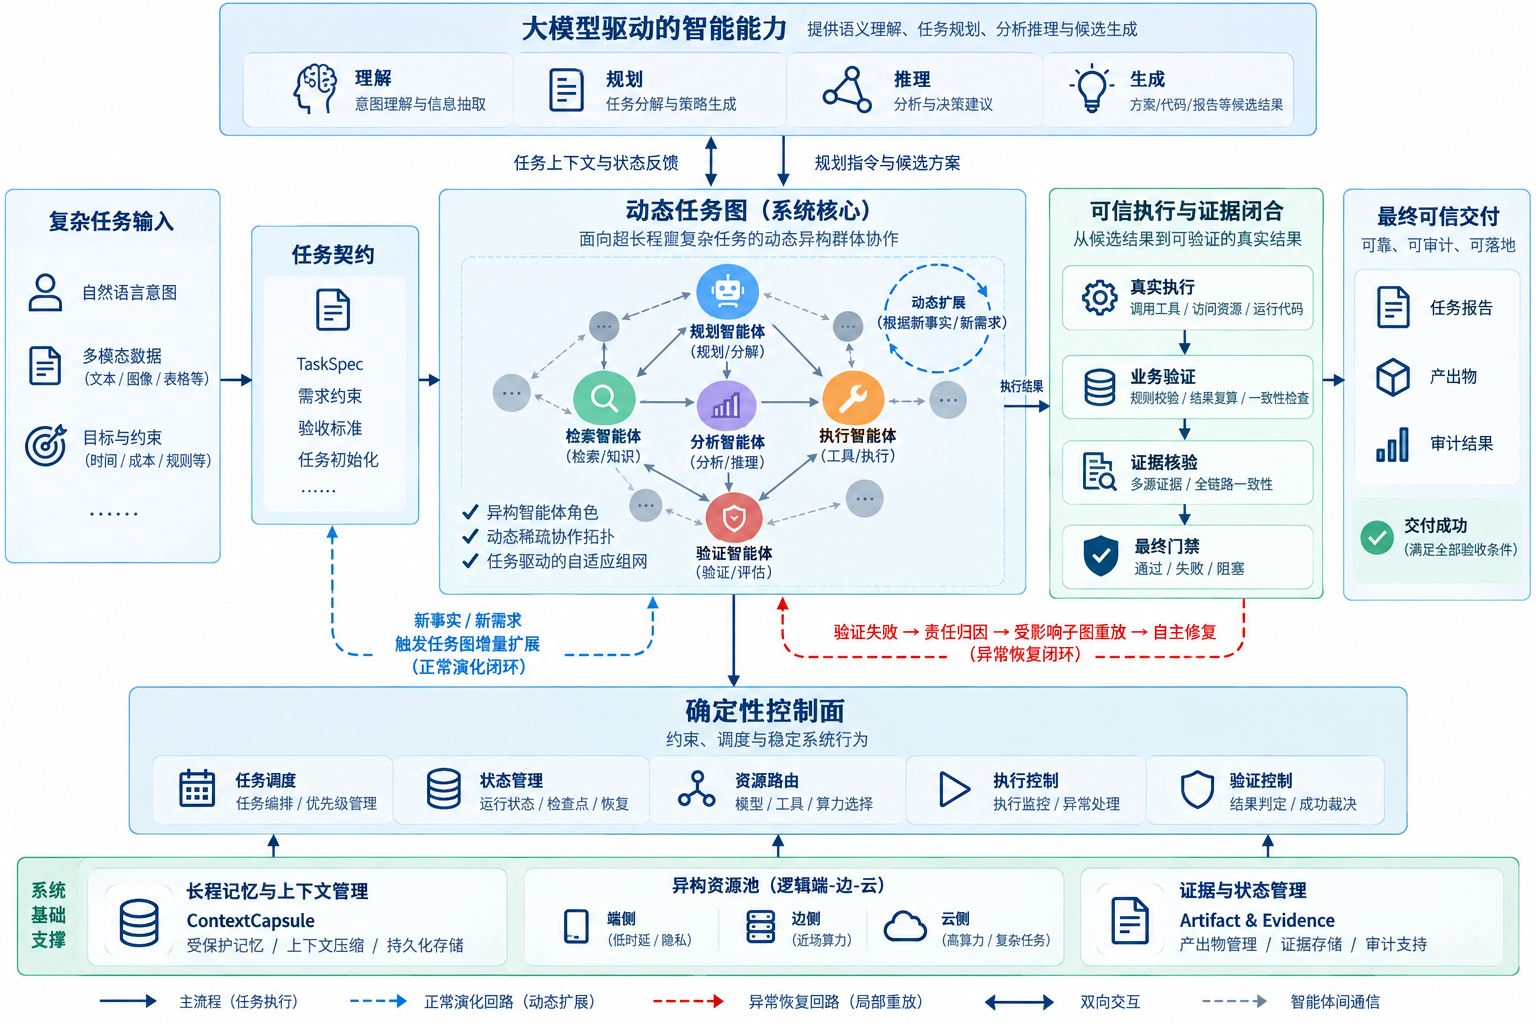
\includegraphics[width=0.98\textwidth]{figures/系统整体流程框架图.png}
\caption{Dynamic-HMAS 总体架构：模型驱动智能面与确定性控制面围绕版本化任务图形成任务执行、可信验收与异常恢复三个闭环。}
\label{fig:integrated-architecture}
\end{figure}

系统进一步划分为六个逻辑职责层。需要说明的是，六层结构并不表示运行时存在固定的六阶段串行流水线，而是对系统职责进行逻辑划分。各层围绕同一个版本化运行状态工作：规划层可以在执行过程中修改后续任务图；记忆层可以向任意节点提供受保护上下文；资源层在每个节点执行前重新完成资源选择；验收层则可以将失败沿证据关系反馈到上游责任节点。因此，系统真正的执行顺序由任务依赖与当前运行状态决定，而不是由固定层次顺序决定。

\subsection{输入与任务契约层}

输入与任务契约层负责将高层自然语言意图转化为控制面能够执行和验收的结构化对象。

系统可接收自然语言以及 PDF、DOCX、XLSX、JSONL、CSV、遥感目录和 PCAP 等异构输入，并识别文件清单、数据格式、敏感等级、时间预算、资源约束和交付格式。

随后系统生成两个核心对象：TaskSpec 和 Requirement Contract。

TaskSpec 描述整个任务的目标、输入摘要、约束集合、允许资源位置、预算和交付物类型；Requirement Contract 则进一步将自然语言要求分解为唯一的 \texttt{requirement\_id}、责任节点、验收条件和证据要求。

任务契约冻结后生成 \texttt{requirement\_digest}。后续任务图版本、checkpoint 和恢复流程均保存该摘要，以检测执行过程中是否出现目标或需求的静默漂移。


\subsection{规划与任务图层}

规划与任务图层负责将任务契约转化为可执行的语义节点和依赖关系。

规划器并不直接输出一条完整固定流水线，而是生成带有能力标签、输入输出契约、安全等级、资源约束、重试策略和证据要求的 TaskNode。Graph Compiler 根据节点依赖构建 DAG，并在执行过程中根据当前需求前沿逐阶段扩展。

每次任务图变更前，控制面执行确定性合法性检查，包括：

\begin{itemize}
    \item 节点 ID 唯一性；
    \item 依赖节点存在性；
    \item 图结构无环性；
    \item 节点权限合法性；
    \item 输入输出契约合法性；
    \item 最终交付节点唯一性。
\end{itemize}

只有通过全部检查的图版本才能进入调度状态。这一机制使同一套任务图和调度语义能够复用于物流、财务和城市多模态等不同领域，而领域差异主要体现在节点能力和验证函数。


\subsection{执行与调度层}

执行与调度层负责将合法任务图转化为实际运行行为。

Scheduler 持续读取当前图版本，寻找满足所有硬依赖、输入契约、权限和资源条件的 ready 节点。节点进入执行前，系统首先构造只读 ContextCapsule，并根据当前资源状态完成执行后端选择。

节点执行完成后，控制面记录：

\begin{itemize}
    \item 标准化节点输出；
    \item 实际执行资源；
    \item 命令或模型调用信息；
    \item 退出码；
    \item 执行耗时；
    \item Token 使用；
    \item artifact 路径及哈希；
    \item 节点状态迁移。
\end{itemize}

调度器为每个 WorkUnit 维护幂等键。恢复时，已经确认完成并通过验证的 WorkUnit 不会重复执行；只有未完成节点或受到异常和需求变更影响的节点及其后继会被重新打开。


\subsection{记忆与通信层}

记忆与通信层负责在长程任务中维持目标、约束、事实和证据的连续性，同时抑制多智能体通信冗余。

系统维护工作记忆、情景记忆、语义记忆、程序记忆和 artifact 记忆，并在每个节点执行前根据节点契约、直接依赖关系和 Token 预算构造只读 ContextCapsule。

通信不采用所有 Agent 共享完整历史的方式，而是依据任务图中的直接依赖发送结构化 MessageEnvelope。通信内容经过字段投影，只包含当前接收节点完成任务所需的结构化输出、摘要、artifact 引用、证据引用和哈希。

大型对象不在 Agent 之间重复传输，而是存储在外部 artifact 空间，并通过路径与哈希引用。SQLite、事件日志和 checkpoint 共同保存长期状态，使节点和进程在重启后仍能够恢复任务语义，而不依赖某个 Agent 的私有上下文。


\subsection{资源与模型层}

资源与模型层负责将 TaskNode 的能力和安全需求映射到实际可用的执行后端。

ResourceRegistry 将端侧、边缘侧和云侧统一抽象为可替换资源描述符，并记录模型名称、资源位置、能力集合、算力、时延、成本、安全等级、并发限制、当前可用性和历史表现。

路由过程首先执行安全、位置、能力、可用性、实时性和算力等硬约束过滤，只有合法资源才能进入候选集合；随后再根据质量、历史成功率、时延、成本、负载和连续失败情况进行软排序。

资源切换只改变节点的执行位置，不允许修改 TaskSpec、Requirement Contract、当前图版本和已经验证的事实。当当前资源不可用时，控制面重新选择合法候选，并将切换原因、旧资源、新资源和执行结果写入事件日志。


\subsection{验收与交付层}

验收与交付层负责将“候选结果”转换为“可信交付结果”。

整个交付过程由四级门禁组成：

\begin{enumerate}
    \item \textbf{业务验证（Business Validation）}：
    Domain Validator 从真实 artifact 中重新计算领域约束和关键业务指标。

    \item \textbf{证据核验（Evidence Verification）}：
    Evidence Verifier 检查声明是否能够闭合到合法来源节点、实际文件、正确图版本和一致哈希。

    \item \textbf{需求验收（Requirement Acceptance）}：
    Requirement Reviewer 检查 Requirement Contract 中的每一个需求是否均有已验证结果支撑。

    \item \textbf{最终门禁（Final Gate）}：
    汇总业务验证、证据核验、需求验收和交付文件状态，仅在所有硬条件满足时写入全局 \texttt{success}。
\end{enumerate}

因此，即使模型已经生成格式完整的报告，只要任何一个硬门禁未通过，系统仍不会将该运行视为成功交付。


\section{统一契约与跨层解耦机制}

Dynamic-HMAS 并不要求各个模块理解彼此内部实现，而是通过四类稳定契约连接模型面与控制面。

\begin{table}[htbp]
\centering
\caption{系统核心契约及其作用}
\label{tab:core-contracts}
\begin{tabularx}{0.96\textwidth}{p{0.21\textwidth}X p{0.28\textwidth}}
\toprule
契约 & 主要内容 & 架构作用\\
\midrule
TaskSpec
& 全局目标、输入、约束、安全等级、预算和交付格式
& 定义整个任务的稳定语义边界\\

TaskNode
& 节点类型、能力、依赖、输入输出 Schema、资源约束、重试和证据要求
& 将开放式任务计划编译为可调度执行单元\\

MessageEnvelope
& 结构化输出、摘要、artifact 引用、证据引用、置信状态和哈希
& 限制节点间信息传播范围，避免全历史自由通信\\

ValidationResult
& 验证状态、错误等级、责任节点、期望值、实际值、artifact 和修复提示
& 将验证结果直接转换为控制面可执行的恢复信号\\
\bottomrule
\end{tabularx}
\end{table}

这些契约不仅承担数据传输功能，也定义了跨层状态边界。上游模型不能通过自然语言文本直接修改下游控制状态；节点只能通过 TaskNode 和 MessageEnvelope 规定的结构化字段影响其他节点；验证器也不通过模糊自然语言建议触发恢复，而是通过结构化 ValidationResult 返回责任节点、错误位置和验收状态。

这一机制带来三项工程收益。

第一，节点实现可以被替换。例如，一个原本由云端模型执行的节点可以切换到边缘模型，而上游规划逻辑无需修改。

第二，领域能力可以插件化接入。新场景只需定义自己的输入适配器、结果 Schema 和 Domain Validator，即可复用统一的 Scheduler、Memory、Evidence 和 Final Gate。

第三，失败归因不需要模型重新阅读全部历史。控制器可以直接依据 ValidationResult 中的 \texttt{owner\_node}、错误字段和 artifact 来源确定后续恢复路径。


\section{任务数据流、控制流与证据流}

Dynamic-HMAS 在运行过程中同时维护数据流、控制流和证据流。三者相互关联，但承担不同职责。

\subsection{任务数据流}

任务数据流回答“内容和结果如何产生”。

其典型路径为：
\[
\begin{aligned}
&\text{Raw Input}
\rightarrow \text{TaskSpec}
\rightarrow \text{Node Output} \\[3pt]
&\qquad\rightarrow \text{Artifact}
\rightarrow \text{Validated Result}
\rightarrow \text{Final Report}.
\end{aligned}
\]

原始输入首先被规范化并形成文件清单和 TaskSpec；节点执行产生结构化输出和 artifact；验证器从实际 artifact 中复算业务事实；Reporter 只读取已经通过验收的结果形成最终文档。

\subsection{控制流}

控制流回答“谁决定系统下一步执行什么”。

控制器依据当前图版本和节点依赖选择 ready 节点，在节点执行前完成 ContextCapsule 构造和资源路由，在执行后依据结果更新节点状态。若验证失败，则根据责任节点和图依赖进入局部恢复路径。

其典型逻辑为：
\[
\text{Dependency}
\rightarrow
\text{Scheduling}
\rightarrow
\text{Routing}
\rightarrow
\text{Execution}
\rightarrow
\text{Validation}
\rightarrow
\text{State Transition}.
\]

\subsection{证据流}

证据流回答“为什么某个结果值得相信”。

每项关键结果都通过
\[
\texttt{node\_id},
\quad
\texttt{artifact\_hash},
\quad
\texttt{graph\_version},
\quad
\texttt{requirement\_id}
\]
连接到其实际生产节点、真实文件、任务图版本和验收要求。

因此，最终报告中的关键声明并不是孤立文本，而能够沿如下链路回溯：
\[
\text{Claim}
\rightarrow
\text{Requirement}
\rightarrow
\text{Producer Node}
\rightarrow
\text{Artifact}
\rightarrow
\text{Hash}
\rightarrow
\text{Validation Result}.
\]

以 MathorCup 装箱任务为例，任务数据流可以表示为：
\[
\begin{aligned}
&\text{题目文件}
\rightarrow \text{货物与车辆规格}
\rightarrow \text{候选 placements} \\[3pt]
&\qquad\rightarrow \texttt{result.json}
\rightarrow \text{约束日志}
\rightarrow \text{成本比较}
\rightarrow \text{最终报告}.
\end{aligned}
\]

控制流则表现为：
\[
\begin{aligned}
&\text{输入规范化}
\rightarrow \text{契约冻结}
\rightarrow \text{任务规划}
\rightarrow \text{真实执行} \\[3pt]
&\qquad\rightarrow \text{领域验证}
\rightarrow \text{证据核验}
\rightarrow \text{需求验收}.
\end{aligned}
\]

如果 \texttt{result.json} 已经生成但约束验证失败，说明数据流已经形成了候选产物，但该产物尚未升级为可信事实。控制流会阻止其进入报告阶段，并将相关责任节点置为失败状态后触发修复。


\section{组件责任与状态写入权限}

为了避免多个 Agent 对全局状态拥有不受约束的修改权，Dynamic-HMAS 对不同组件的职责和状态写入权限进行显式划分。

\begin{table}[htbp]
\centering
\caption{核心组件的责任边界与状态写入权限}
\label{tab:component-permission}
\begin{tabularx}{0.97\textwidth}{p{0.19\textwidth}X p{0.25\textwidth}p{0.11\textwidth}}
\toprule
组件 & 核心职责 & 可写入对象 & 全局 success\\
\midrule
Planner / Analyst
& 意图理解、任务拆解、候选规划和专业分析
& 候选计划、分析结果
& 否\\

Graph Compiler
& 将语义计划转换为合法 DAG，并执行依赖和契约校验
& 图版本及合法性结果
& 否\\

Scheduler / Router
& ready 节点调度、状态迁移、资源选择和故障回退
& 节点状态、路由记录
& 否\\

Code Generator
& 根据节点契约生成候选代码和运行建议
& 代码候选
& 否\\

Terminal Executor
& 在受控环境真实运行代码或工具
& stdout、stderr、exit code、artifact
& 否\\

Domain Validator
& 对实际 artifact 执行确定性业务复算
& business validation
& 否\\

Evidence Verifier
& 检查来源、文件、版本和哈希一致性
& evidence validation
& 否\\

Requirement Reviewer
& 检查需求账本是否全部闭合
& requirement ledger
& 否\\

Reporter
& 基于已验证事实组织最终文档
& 文档候选
& 否\\

Final Gate
& 汇总所有硬门禁并裁决最终结果
& global outcome
& 是\\
\bottomrule
\end{tabularx}
\end{table}

该权限体系形成“\textbf{模型可以提出候选，但不能定义事实；执行器可以产生事实，但不能宣布成功；验证器可以确认局部正确性，但不能单独决定全局结果；只有 Final Gate 可以写入全局 outcome}”的责任链。

这种权限分离是可信执行的基础，也为后续错误归因提供明确的 producer 和 owner 边界。


\section{运行状态机与异常恢复}

系统以统一状态机管理一次完整运行。主要状态如表~\ref{tab:run-state-machine} 所示。

\begin{table}[htbp]
\centering
\caption{一次完整运行的主要状态}
\label{tab:run-state-machine}
\begin{tabularx}{0.94\textwidth}{p{0.20\textwidth}X}
\toprule
状态 & 进入条件与主要动作\\
\midrule
\texttt{prepare}
& 创建运行目录、输入清单、事件日志、密钥隔离和初始 checkpoint。\\

\texttt{classify}
& 识别领域、数据敏感等级、交付类型、预算和验收规则。\\

\texttt{plan}
& 生成或扩展 DAG，并执行环检测、权限检查及唯一交付节点校验。\\

\texttt{execute}
& 调度 ready 节点，唤醒记忆、完成资源路由并执行模型、代码或工具。\\

\texttt{review}
& 执行业务验证、证据核验和需求验收；失败时进入责任归因与局部恢复。\\

\texttt{report}
& 仅在前置硬门禁满足后生成最终交付文档。\\

\texttt{final\_validate}
& 校验报告、artifact 哈希、节点状态及阻塞问题，并生成最终 outcome。\\

\texttt{finish}
& 固化运行状态、指标和审计结果，供 Dashboard 和提交包读取。\\
\bottomrule
\end{tabularx}
\end{table}

需要强调的是，\texttt{report} 并非默认可达状态。只有业务验证、证据核验和需求验收满足前置要求后，系统才允许进入报告阶段；同样，报告生成也不意味着任务已经成功，仍需经过最终交付校验和 Final Gate。

正常执行路径可以概括为：
\[
\begin{aligned}
&\text{输入规范化}
\rightarrow \text{契约冻结}
\rightarrow \text{阶段规划}
\rightarrow \text{DAG 校验}
\rightarrow \text{依赖调度} \\[3pt]
&\qquad\rightarrow \text{真实执行}
\rightarrow \text{业务验证}
\rightarrow \text{证据核验}
\rightarrow \text{需求验收}
\rightarrow \text{最终交付}.
\end{aligned}
\]

异常恢复被建模为正常状态机中的一等控制路径，而不是附加在主流程之外的 retry 脚本。当节点失败后，系统首先记录原始错误、节点 ID、图版本和关联 artifact，并根据错误类型和来源信息确定责任节点。若错误可恢复，则仅将责任节点及其受影响后继重新打开；若资源不可用，则重新执行资源候选选择；若需求发生变化，则产生新的图版本；若输入副本损坏，则执行隔离、哈希确认和数据恢复。

正常执行和异常恢复共享相同的 Scheduler、状态存储、版本体系、记忆和最终验收门禁。重试预算耗尽或不存在合法恢复路径时，系统明确进入 \texttt{failed} 或 \texttt{blocked}，而不是生成假成功结果。具体的错误分类、责任归因、RepairContext 和受影响子图重放机制将在第六章进一步展开。


\section{动态任务图与版本一致性}

Dynamic-HMAS 使用版本化任务图维护长程运行过程中任务结构和任务语义的一致性。

图版本 $G_t$ 与 \texttt{requirement\_digest}、memory snapshot、artifact 清单及其哈希共同绑定。版本号不仅用于标识任务图结构，也构成任务语义、记忆状态和执行事实之间的一致性边界。

当用户需求发生变化时，系统不会直接修改历史图，而是产生新的图版本
\[
G_{t+1},
\]
并根据变化影响范围标记需要重新打开的节点。未受影响且已经验证的节点继续保持冻结，其 artifact 可以在新图版本中按照明确规则继续引用。

恢复时，Scheduler 根据 checkpoint、节点幂等键和当前图版本判断哪些 WorkUnit 已经完成，从而避免对已验证任务进行重复执行。

该机制具有三项作用：

\begin{enumerate}
    \item 防止新需求静默覆盖旧需求，使历史任务语义仍可审计；
    \item 防止旧 artifact 被错误用于新图版本；
    \item 支持中断恢复后从正确状态继续，而不是从头重新计算。
\end{enumerate}

因此，评审者可以通过 \texttt{task\_graph.json}、\texttt{run\_state.json}、checkpoint 和事件日志复核每一次图扩展、版本变化、节点重开和状态迁移。


\section{机器可审计的运行证据}

Dynamic-HMAS 将可审计性设计为运行时属性，而不是依赖 Dashboard 截图或模型文字说明。

每次任务运行至少保存：

\begin{itemize}
    \item \texttt{run\_state.json}：记录全局 outcome、节点状态、图版本、资源路由、Token、重试与验收状态；
    \item \texttt{task\_graph.json}：记录任务节点、依赖关系和图版本；
    \item \texttt{agent\_trace.md}：保存模型和智能体的中间决策摘要；
    \item \texttt{events.jsonl}：保存状态迁移、异常、资源切换和恢复事件；
    \item \texttt{artifacts/}：保存真实执行产生的结构化结果；
    \item \texttt{review/}：保存业务、证据和需求验收结果；
    \item \texttt{checkpoints/}：保存长程恢复快照；
    \item \texttt{injections/}：保存动态异常注入及恢复轨迹。
\end{itemize}

关键 artifact 和 checkpoint 均保存 SHA256 等一致性信息，使运行结果可以脱离前端界面独立复核。

因此，Dashboard 的作用是将节点状态、路由、轨迹、artifact 和验收结果可视化，而不是充当系统真值来源。系统是否成功最终由机器可读 RunState、验证文件和 Final Gate 决定。

这种“前端负责观察、机器状态负责裁决”的设计也降低了系统对复杂交互界面的依赖：即使可视化界面较为轻量，完整运行过程仍然能够通过底层状态和证据文件被重新检查。


\section{本章小结}

本章给出了 Dynamic-HMAS 的总体系统架构。其核心并不在于简单增加 Agent 数量或堆叠更多功能模块，而在于通过\textbf{模型驱动智能面与确定性控制面的职责分离}，将开放式模型能力约束在显式契约、版本化任务图和确定性状态机之内。

基于该双平面结构，系统形成任务闭环、可信闭环和恢复闭环：任务闭环负责将高层意图持续编译和扩展为可执行任务图；可信闭环负责将模型候选通过真实执行、业务验证和证据核验转化为可信事实；恢复闭环负责在异常发生后沿事实和证据来源定位责任节点，并在保持未受影响状态的前提下完成局部恢复。

六层逻辑架构进一步划分系统职责，而 TaskSpec、TaskNode、MessageEnvelope 和 ValidationResult 提供跨层稳定契约。任务数据流、控制流和证据流分别描述内容如何产生、系统如何决策以及结果为何可信，并通过节点标识、图版本、artifact 哈希和需求编号保持一致关联。

上述架构使 Dynamic-HMAS 区别于静态 Agent 流水线：任务结构可以随着执行事实动态演化，模型不能直接修改全局成功状态，资源切换不会破坏任务语义，验证失败也能够进入统一状态机中的恢复路径。后续章节将在该总体架构基础上进一步展开动态异构群体与深度协同推理、长程上下文保持、端边云异构资源路由以及验证驱动的可信执行与自主修复机制。

\chapter{动态异构群体组织与深度协同推理}

本章讨论 Dynamic-HMAS 如何将一组能力、资源、可靠性与信息权限不同的执行单元组织为可动态重组的智能群体，并进一步说明系统如何基于任务图、结构化消息和执行反馈形成跨阶段的深度协同推理机制。

本文所称的“群体”并不等价于多个模型同时输出文本，也不以 Agent 数量或自由对话轮次衡量协作能力。系统真正管理的是角色能力、任务依赖、资源位置、信息权限与结果责任之间的组合关系。节点是否加入当前任务图、何时进入执行状态、可以读取哪些信息、使用何种资源以及失败后是否需要重新激活，均由任务图和确定性控制面共同决定。

与静态多智能体流水线不同，Dynamic-HMAS 不假设一次规划即可预见全部执行步骤。系统以版本化任务图为协作载体，根据中间执行结果、需求变化和异常反馈逐阶段扩展任务结构；模型节点负责开放式语义理解、规划与候选生成，控制面负责依赖、状态、资源、真实执行和验证约束。执行与验证产生的新事实进一步改变后续任务图及节点上下文，从而形成“候选推理—真实执行—事实验证—状态更新—继续推理”的闭环。

\begin{figure}[htbp]
\centering
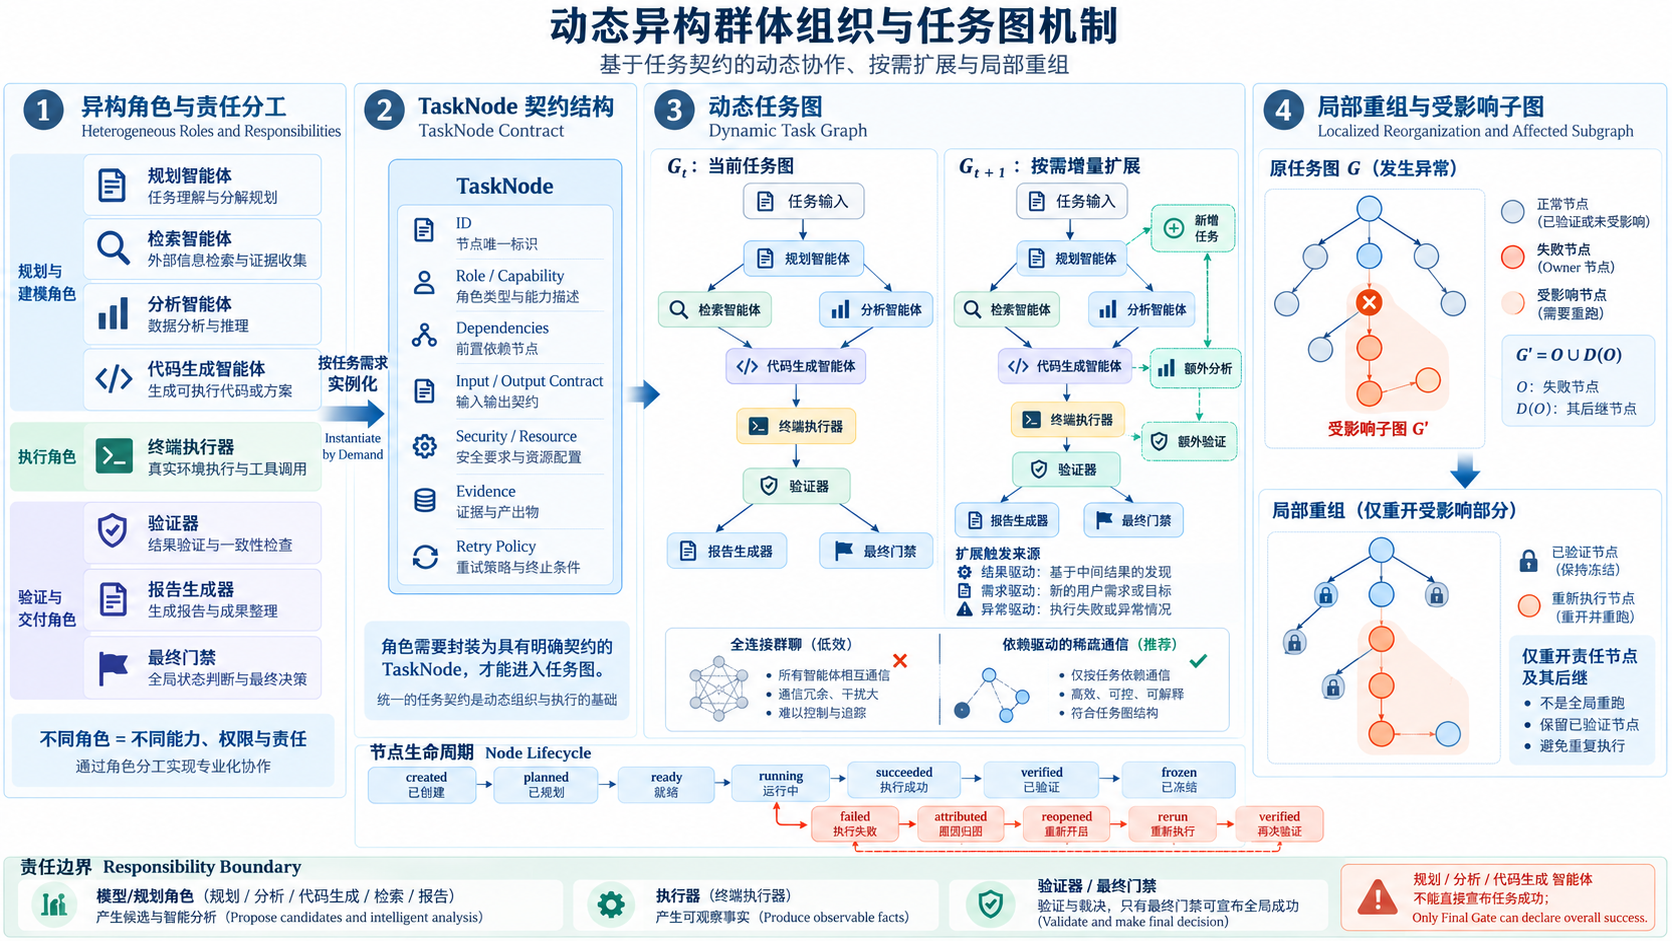
\includegraphics[width=0.98\textwidth]{figures/动态异构群体组织与任务图协作机制.png}
\caption{动态异构群体组织与任务图机制：角色契约实例化、依赖驱动协作、按需增量扩展以及受影响子图局部重组。}
\label{fig:dynamic-heterogeneous-task-graph}
\end{figure}


\section{异构性的四个维度}

Dynamic-HMAS 中的异构性并非仅指使用不同的大模型，而是由能力、资源、可靠性和信息权限四个相互关联的维度共同构成。

\textbf{能力异构}指规划、检索、分析、代码生成、终端执行、领域验证、证据核验和报告编排等节点承担不同职责。不同节点并不要求由不同模型实现，同一模型也可以在不同 TaskNode 契约下承担不同角色。

\textbf{资源异构}指同一种能力可以绑定不同执行后端，例如本地工具、端侧模型、边缘服务或云端模型。任务图只描述“当前节点需要什么能力”，具体由哪个资源执行，则由第五章介绍的 ResourceRegistry 和资源路由机制决定。

\textbf{可靠性异构}指不同执行资源在成功率、时延、成本、可用性和历史失败情况等方面存在差异。可靠性不是 TaskNode 的固定静态属性，而是绑定执行资源的运行时状态，由资源注册表持续记录，并在资源候选过滤与排序阶段参与决策。

\textbf{信息权限异构}指不同节点拥有不同的信息可见范围。节点只能读取完成当前任务所需的字段、直接依赖结果及经过授权的外部记忆，敏感原始数据和全局状态不会无条件暴露给所有 Agent。

上述定义使系统避免“以 Agent 数量衡量群体规模”的简单思路。系统真正管理的是能力、资源、信息和责任的组合，并通过显式任务图将这些组合关系结构化。新增一个模型并不会自动改变群体结构，只有当其注册了合法能力、资源约束并满足当前节点的安全与证据要求后，才可能被调度器选中。


\section{角色体系与责任分工}

\begin{table}[htbp]
\centering
\caption{Dynamic-HMAS 的主要角色及责任边界}
\label{tab:agent-role-responsibility}
\begin{tabular}{p{0.22\textwidth}p{0.42\textwidth}p{0.22\textwidth}}
\toprule
角色 & 主要责任 & 结果性质\\
\midrule
Planner & 意图理解、目标拆解、阶段计划建议 & 候选计划\\
Retriever & 文件解析、检索和证据提取 & 结构化证据\\
Analyst & 领域分析、比较和推理 & 候选结论\\
Code Generator & 根据节点契约生成可执行代码 & 代码候选\\
Terminal Executor & 在受控环境执行代码或工具 & 进程结果与 artifact\\
Domain Validator & 对领域结果进行确定性复算 & 业务验证结论\\
Evidence Verifier & 检查声明、文件、节点和哈希闭合 & 证据验证结论\\
Reporter & 基于已验证事实生成交付文档 & 文档候选\\
Governance / Final Gate & 管理状态、预算、权限并裁决最终结果 & 全局状态\\
\bottomrule
\end{tabular}
\end{table}

角色设计的核心目的不是增加智能体数量，而是建立明确的责任边界。

Planner 可以提出不完整或需要后续修正的任务计划，但不能宣布任务成功；Code Generator 可以生成语法正确的程序，但其输出仍然只是候选代码，不能替代 Terminal Executor 的真实执行；Reporter 可以组织最终文档，但只能读取已经通过验收的事实；Domain Validator 和 Evidence Verifier 分别负责业务正确性与证据一致性，也不能单独写入全局成功状态。

只有 Final Gate 在业务验证、证据核验、需求验收和交付校验均满足时，才有权将全局 outcome 写为 success。该责任分离避免了多智能体系统中常见的责任漂移，也防止模型通过语言表达覆盖底层执行或验证事实。


\section{层级化群体组织}

系统采用“全局治理层—阶段协同层—原子执行层”的三级组织结构。

\textbf{全局治理层}维护 TaskSpec、Requirement Contract、任务图版本、全局预算、状态账本和最终交付门禁。该层回答“整个任务最终需要完成什么、哪些要求仍未闭合以及系统是否允许交付”。

\textbf{阶段协同层}围绕输入理解、数据准备、规划、分析、执行、验证和交付等阶段动态生成局部子图。阶段协同层并非预先固定的组织结构，而是随着当前需求前沿和中间事实变化动态创建和释放。

\textbf{原子执行层}负责文件解析、检索、统计计算、代码运行、几何验证、金额复算、证据扫描等具有明确输入输出契约的实际操作，并向上层返回可观察结果。

三级组织不是固定的行政层级，而是运行时的责任边界。全局治理层维护任务目标和需求状态，阶段协同层决定下一阶段需要哪些能力，原子执行层产生真实可观察事实。当阶段完成后，对应的协同结构可以冻结；若验证失败，控制器只重新激活包含责任节点的受影响子图，而不会让整个群体回到初始状态。


\section{任务节点模型与契约}

系统将每一个可执行任务单元统一表示为 TaskNode。第 $i$ 个节点定义为
\[
v_i=
(id_i,type_i,cap_i,dep_i,in_i,out_i,sec_i,res_i,ev_i,retry_i),
\]
其中：

\begin{itemize}
    \item $id_i$ 表示节点唯一标识；
    \item $type_i$ 表示节点角色类型；
    \item $cap_i$ 表示节点所需能力标签；
    \item $dep_i$ 表示硬依赖节点集合；
    \item $in_i$ 和 $out_i$ 分别表示输入与输出契约；
    \item $sec_i$ 表示安全与信息权限要求；
    \item $res_i$ 表示计算资源和执行位置约束；
    \item $ev_i$ 表示输出结果必须满足的证据要求；
    \item $retry_i$ 表示重试策略和预算。
\end{itemize}

节点只有在所有硬依赖均已满足、信息权限合法、输入 Schema 通过且存在可用资源时，才能进入 ready 状态。形式上，可将节点就绪条件表示为
\[
Ready(v_i,t)=
\mathbf{1}
\left[
dep_i\subseteq V_t^{verified}
\land
Permission_i(t)
\land
Schema_i(t)
\land
Resource_i(t)
\right],
\]
其中 $V_t^{verified}$ 表示时刻 $t$ 已通过验证的节点集合。

TaskNode 契约将“节点应该做什么”和“节点实际做了什么”分开管理。输入契约限制当前节点能够读取的字段和文件范围，输出契约规定 Schema、必填字段及 artifact 类型，证据契约规定结果必须由哪些来源和产物支撑。由此，即使同一角色由不同模型或不同资源实现，下游节点仍然可以按照统一契约消费结果，而无需理解上游模型内部的提示词和推理过程。


\section{动态任务图生成与增量扩展}

在运行时刻 $t$，系统维护版本化任务图
\[
G_t=(V_t,E_t),
\]
其中 $V_t$ 表示当前所有任务节点，$E_t$ 表示节点之间允许的直接依赖关系。

初始任务图由冻结后的 TaskSpec 和 Requirement Contract 编译得到，但系统并不假设一次规划能够提前预见全部执行步骤。为描述仍需处理的任务需求，定义未闭合需求前沿
\[
\mathcal{F}_t=
\left\{
q_i\in Q_t
\mid
status(q_i)\neq passed
\right\},
\]
其中 $Q_t$ 为当前需求验收账本。

规划器根据需求前沿 $\mathcal{F}_t$、当前记忆状态 $M_t$、已有产物集合 $A_t$ 和当前任务图 $G_t$ 生成候选增量子图：
\[
\Delta G_t=
\Pi
\left(
\mathcal{F}_t,
M_t,
A_t,
G_t
\right),
\]
其中 $\Pi(\cdot)$ 表示规划模型根据当前状态产生候选节点及依赖关系的过程。

候选增量图不能直接进入运行状态。控制面首先执行节点 ID 唯一性、依赖存在性、无环性、权限约束、输入输出契约及唯一交付节点等检查。只有合法的增量图才能被合并：
\[
G_{t+1}
=
Validate
\left(
G_t\oplus\Delta G_t
\right).
\]

这里的 $Validate(\cdot)$ 并非语言模型判断，而是控制面执行的确定性图结构检查；若候选扩展不合法，则保留原图版本并记录失败原因。

动态图扩展主要包含三类触发来源。

\textbf{结果驱动扩展}：上游执行产生新的事实，表明仍需要进一步检索、分析、代码生成或补充验证。

\textbf{需求驱动扩展}：用户在执行过程中增加新的输出字段、比较目标或约束，系统生成新的图版本并仅重开受到影响的节点。

\textbf{异常驱动扩展}：领域验证、资源调用或输入数据出现异常，需要加入错误分析、修复、重新执行或复验节点。

扩展后的任务图以新版本保存，旧版本不会被静默覆盖。图版本与 requirement digest、memory snapshot 和 artifact hash 共同绑定，从而保证任务结构发生变化后仍然能够追踪其来源。

\begin{algorithm}[H]
\caption{版本化任务图的增量扩展}
\label{alg:incremental-graph-expansion}

\KwIn{当前任务图 $G_t$，需求前沿 $\mathcal{F}_t$，记忆状态 $M_t$，产物集合 $A_t$}
\KwOut{新图版本 $G_{t+1}$ 或保持 $G_t$}

根据 $\mathcal{F}_t$ 确定尚未闭合的能力与证据需求\;

$\Delta G_t \leftarrow \Pi(\mathcal{F}_t,M_t,A_t,G_t)$\;

检查候选节点 ID 唯一性\;

检查所有依赖节点是否存在\;

检查 $G_t\oplus\Delta G_t$ 是否为 DAG\;

检查节点权限、输入输出契约和交付节点唯一性\;

\If{任一合法性检查失败}{
    记录扩展失败原因\;
    $G_{t+1}\leftarrow G_t$\;
}
\Else{
    $G_{t+1}\leftarrow G_t\oplus\Delta G_t$\;
    保存新图版本及其 requirement digest\;
}

\Return{$G_{t+1}$}\;

\end{algorithm}


\section{深度协同推理与低熵通信机制}

\subsection{神经--符号深度协同推理}

本文所称的\textbf{深度协同推理}，并非通过增加多个智能体之间的自由对话轮次来获得，而是指多个异构角色沿动态任务图的依赖关系持续交换结构化事实，并由模型推理、真实执行和符号验证共同推动任务状态演化。

其中，模型驱动智能面负责开放式能力，包括自然语言意图理解、任务拆解、信息分析、方案比较、代码生成以及修复候选生成；确定性控制面负责符号化约束，包括任务依赖、权限、资源合法性、运行状态、真实执行、业务规则、证据一致性和最终成功判定。

对于节点 $v$，控制面首先依据其 TaskNode 契约、直接依赖结果以及长程记忆构造当前上下文
\[
C_v^{(t)}
=
Assemble
\left(
contract(v),
Dep(v),
M_t
\right).
\]
模型基于该上下文产生候选结果
\[
y_v=
Model
\left(
C_v^{(t)}
\right),
\]
候选结果随后由实际执行器转化为可观察结果
\[
a_v=
Execute(y_v),
\]
再由确定性验证器产生验证结果
\[
z_v=
Validate(a_v).
\]

当验证通过时，新的 artifact、证据和结构化事实被写回 $A_{t+1}$、$M_{t+1}$ 和需求账本 $Q_{t+1}$；当验证失败时，结构化错误反馈到责任节点，并触发后续图扩展或局部修复。因此，系统形成如下闭环：
\[
\begin{aligned}
&\text{Model Proposal}
\rightarrow \text{TaskNode}
\rightarrow \text{Execution}
\rightarrow \text{Observable Fact} \\[3pt]
&\qquad\rightarrow \text{Validation}
\rightarrow \text{Graph Update}
\rightarrow \text{New Reasoning}.
\end{aligned}
\]

上述机制使协同推理不再停留于模型间文本交流，而是将模型候选、执行事实、确定性验证和图状态更新统一到同一运行闭环中。这里的“深度”主要体现为跨阶段、跨角色和跨状态版本的持续推理关系，而非单次模型调用内部推理链长度。


\subsection{依赖驱动的低熵结构化通信}

Dynamic-HMAS 不允许所有 Agent 默认读取完整任务历史，也不建立静态全连接群聊。需要区分\textbf{任务依赖图}和\textbf{实际通信拓扑}。

任务图
\[
G_t=(V_t,E_t)
\]
定义节点之间所有合法的直接依赖关系；运行时只有当前被激活并真正发生信息传输的边构成实际通信边集合
\[
E_t^{comm}\subseteq E_t.
\]
因此运行时通信拓扑表示为
\[
G_t^{comm}
=
(V_t,E_t^{comm}).
\]

对于任务图中存在直接依赖关系 $(u,v)\in E_t$ 的节点，上游节点 $u$ 不向节点 $v$ 发送完整历史，而只传递满足其输入契约的最小必要信息。结构化消息可以表示为
\[
m_{u\rightarrow v}
=
\left(
P_v(o_u),
s_u,
R_u^{artifact},
R_u^{evidence},
c_u,
h_u
\right),
\]
其中 $o_u$ 为节点 $u$ 的结构化输出，$P_v(\cdot)$ 表示依据节点 $v$ 输入契约执行的字段投影，$s_u$ 表示必要摘要，$R_u^{artifact}$ 与 $R_u^{evidence}$ 分别表示产物引用和证据引用，$c_u$ 表示结果置信或状态信息，$h_u$ 表示内容哈希。

大型文件和重复对象不会在消息中重复传递正文，而是外置保存，并通过路径、artifact reference 和 hash reference 复用。由此，通信规模主要由实际依赖关系决定，而不是由智能体总数和完整历史长度决定。

本文所称“低熵通信”是面向多智能体工程协作的\textbf{信息冗余控制概念}，并不直接等价于 Shannon 信息熵。本文主要使用活跃通信边数量、通信拓扑密度、平均输入上下文、Token 消耗和全历史广播次数等可观测指标衡量通信冗余。

对于包含 $N_t=|V_t|$ 个节点的任务图，可定义当前通信拓扑密度为
\[
\rho_t
=
\frac{|E_t^{comm}|}
{N_t(N_t-1)}.
\]
当 $\rho_t$ 显著低于 $1$ 且不存在全历史广播时，说明系统的实际通信结构保持稀疏。第七章将使用代表性运行中的实际通信边数、理论全连接边数和上下文规模对该机制进行验证。


\section{节点生命周期与调度规则}

节点生命周期采用显式状态机进行管理。正常执行路径为
\[
created
\rightarrow
planned
\rightarrow
ready
\rightarrow
running
\rightarrow
succeeded
\rightarrow
verified
\rightarrow
frozen.
\]

其中，\texttt{succeeded} 表示节点执行过程本身已经完成并产生结果，但该结果尚未获得领域验证；只有在业务与证据条件满足后才能进入 \texttt{verified}。当结果被后续阶段稳定引用且不再允许普通流程修改时，节点进入 \texttt{frozen} 状态。

异常路径为
\[
running
\rightarrow
failed
\rightarrow
attributed
\rightarrow
reopened
\rightarrow
rerun
\rightarrow
verified.
\]

调度器遵循以下基本规则：

\begin{enumerate}
    \item 硬依赖未满足的节点不得进入 ready；
    \item 权限、输入契约或资源条件不满足的节点不得执行；
    \item 同一幂等键对应的已验证 WorkUnit 不得重复执行；
    \item 仅执行成功但尚未验证的结果不得进入最终交付；
    \item 每次修复或重新执行均必须消耗显式重试预算；
    \item 当重试预算耗尽或不存在合法执行资源时，节点进入 blocked 或 failed 状态。
\end{enumerate}

所有状态迁移均追加到事件日志，并与当前图版本、节点 ID、artifact hash 和重试预算关联，从而使正常执行、异常恢复和后续审计使用同一状态语义。


\section{协同冲突的裁决规则}

异构节点可能针对同一事实产生不同候选结果。为了避免多个 Agent 依据不同事实版本继续传播冲突，系统采用确定性的事实优先级进行裁决。

第一，真实终端执行结果优先于模型推理文本。模型关于“代码已经运行”或“结果满足条件”的自然语言描述不能替代 Terminal Executor 的真实进程状态。

第二，领域验证器基于 artifact 复算得到的业务结论优先于生成器自报的约束满足结果。

第三，在需求发生变化后，新图版本下重新生成并验证的事实优先于旧版本结果，旧结果保留用于审计但不继续覆盖当前状态。

第四，直接依赖节点产生的结构化结果优先于通过多级自然语言转述得到的间接信息。

第五，如果以上规则仍无法消解事实冲突，则系统将相关节点或需求置为 failed 或 blocked，并保留冲突记录，而不是任意选择某一个候选结果继续执行。

该裁决顺序使系统中的“事实”具有稳定来源，并为长程记忆更新和后续责任归因提供一致基础。


\section{受影响子图与局部重组}

当验证器或执行器能够将失败归因到一个或多个责任节点时，系统不会默认重新执行整张任务图。

设责任节点集合为
\[
O\subseteq V,
\]
其所有后继节点构成后继闭包 $D(O)$，则受影响节点集合定义为
\[
V'
=
O\cup D(O),
\]
对应的受影响子图为
\[
G'
=
(V',E'),
\qquad
E'
=
\{(u,v)\in E\mid u,v\in V'\}.
\]

恢复时仅将 $V'$ 中的节点重新标记为可执行状态，而
\[
V\setminus V'
\]
中已经通过验证的节点继续保持 frozen，其 artifact、证据和状态均被保留。

该机制使群体组织具有局部重构能力。例如，当 MathorCup 场景中某一代码节点生成的 placement 出现坐标越界时，只需要重开责任代码节点、Terminal Executor、对应领域验证和后继证据节点，而无需重新执行与该错误无关的已验证任务。

本节只描述任务图层面的局部重组规则。关于 ValidationError 如何确定责任节点、如何构造 RepairContext、重新生成 artifact 并完成完整再验收，将在第六章的验证驱动自主修复机制中进一步讨论。


\section{跨场景组织实例}

尽管不同任务的输入数据、领域规则和验收函数差异显著，但 Dynamic-HMAS 复用相同的角色契约、任务图、调度、记忆与验收基础设施。三个代表性场景的组织方式如表~\ref{tab:cross-domain-role-example} 所示。

\begin{table}[htbp]
\centering
\caption{不同任务场景下的动态群体组织实例}
\label{tab:cross-domain-role-example}
\begin{tabular}{@{}>{\raggedright\arraybackslash}p{0.17\textwidth}>{\raggedright\arraybackslash}p{0.34\textwidth}>{\raggedright\arraybackslash}p{0.24\textwidth}>{\raggedright\arraybackslash}p{0.17\textwidth}@{}}
\toprule
场景 & 主要协作链路 & 领域特有能力 & 复用机制\\
\midrule
MathorCup 装箱
&
约束提取 $\rightarrow$ 方案规划 $\rightarrow$ 代码生成 $\rightarrow$ 真实执行 $\rightarrow$ 几何/数量验证 $\rightarrow$ 成本复算
&
三维边界、AABB 重叠、易碎规则、车辆成本
&
TaskNode、Scheduler、Memory、Final Gate
\\

差旅报销
&
票据解析 $\rightarrow$ 金额汇总 $\rightarrow$ 政策核验 $\rightarrow$ 异常识别 $\rightarrow$ 证据报告
&
金额、日期、票据与政策规则验证
&
TaskNode、Scheduler、Memory、Final Gate
\\

城市多模态
&
来源处理 $\rightarrow$ 数据统计 $\rightarrow$ 跨模态综合 $\rightarrow$ 结果验证 $\rightarrow$ 报告生成
&
遥感元数据、法规、匿名通联与 PCAP 包头统计
&
TaskNode、Scheduler、Memory、Final Gate
\\
\bottomrule
\end{tabular}
\end{table}

三个场景中变化的是输入适配器、节点所需能力以及领域确定性验证函数，不变的是任务节点契约、依赖驱动调度、上下文管理、artifact 管理、状态机和最终验收逻辑。因此，系统的跨场景复用并不是简单复用同一组提示词，而是复用统一的任务与控制语义。


\section{本章小结}

本章建立了 Dynamic-HMAS 的动态异构群体组织与深度协同推理机制。系统不以 Agent 数量或自由对话轮次衡量群体能力，而是通过角色契约、版本化任务图和运行时责任边界组织不同能力、资源、可靠性和信息权限的执行单元。

初始任务图由 TaskSpec 和 Requirement Contract 编译得到，并根据结果、需求变化和异常反馈按需增量扩展；实际通信仅沿当前激活的直接依赖边传递满足下游输入契约的结构化信息，以字段投影、artifact 引用和哈希引用避免全历史广播和大型对象重复传输。

在此基础上，模型节点负责开放式语义理解、规划和候选生成，确定性控制面负责依赖、权限、状态、执行和验证约束；真实执行与验证产生的新事实进一步驱动任务图和上下文更新，从而形成跨角色、跨阶段和跨图版本的深度协同推理闭环。当节点失败时，系统仅重开责任节点及其后继构成的受影响子图，并保留其他已经验证的结果。

后续章节将在上述组织框架基础上进一步讨论长程记忆与 ContextCapsule、端边云异构资源路由，以及验证驱动的可信执行和自主修复机制。

\chapter{长程状态记忆与上下文保持}

本章研究超长程复杂任务中的状态连续性问题。Dynamic-HMAS 的目标并不是让某个大模型“记住更多文本”，而是将任务目标、硬约束、中间事实、图版本、artifact 来源和验收状态从模型上下文中分离出来，转化为由确定性控制面维护的外部状态，并在每个任务节点执行前构造与其职责相匹配的最小充分上下文。

本章的核心并非设计更多记忆类型，而是建立一种\textbf{受保护、预算有界、版本一致且可恢复的长程状态机制}。其中，受保护状态保证影响正确性的关键约束不会因摘要、压缩或 Token 截断而丢失；ContextCapsule 在固定上下文预算下组合任务契约、直接依赖结果、关键状态与相关记忆；语义 checkpoint 则保存任务图、记忆、artifact 和验收状态，使系统在进程中断后能够恢复完整任务语义，而不仅是恢复程序执行位置。

\begin{figure}[htbp]
\centering
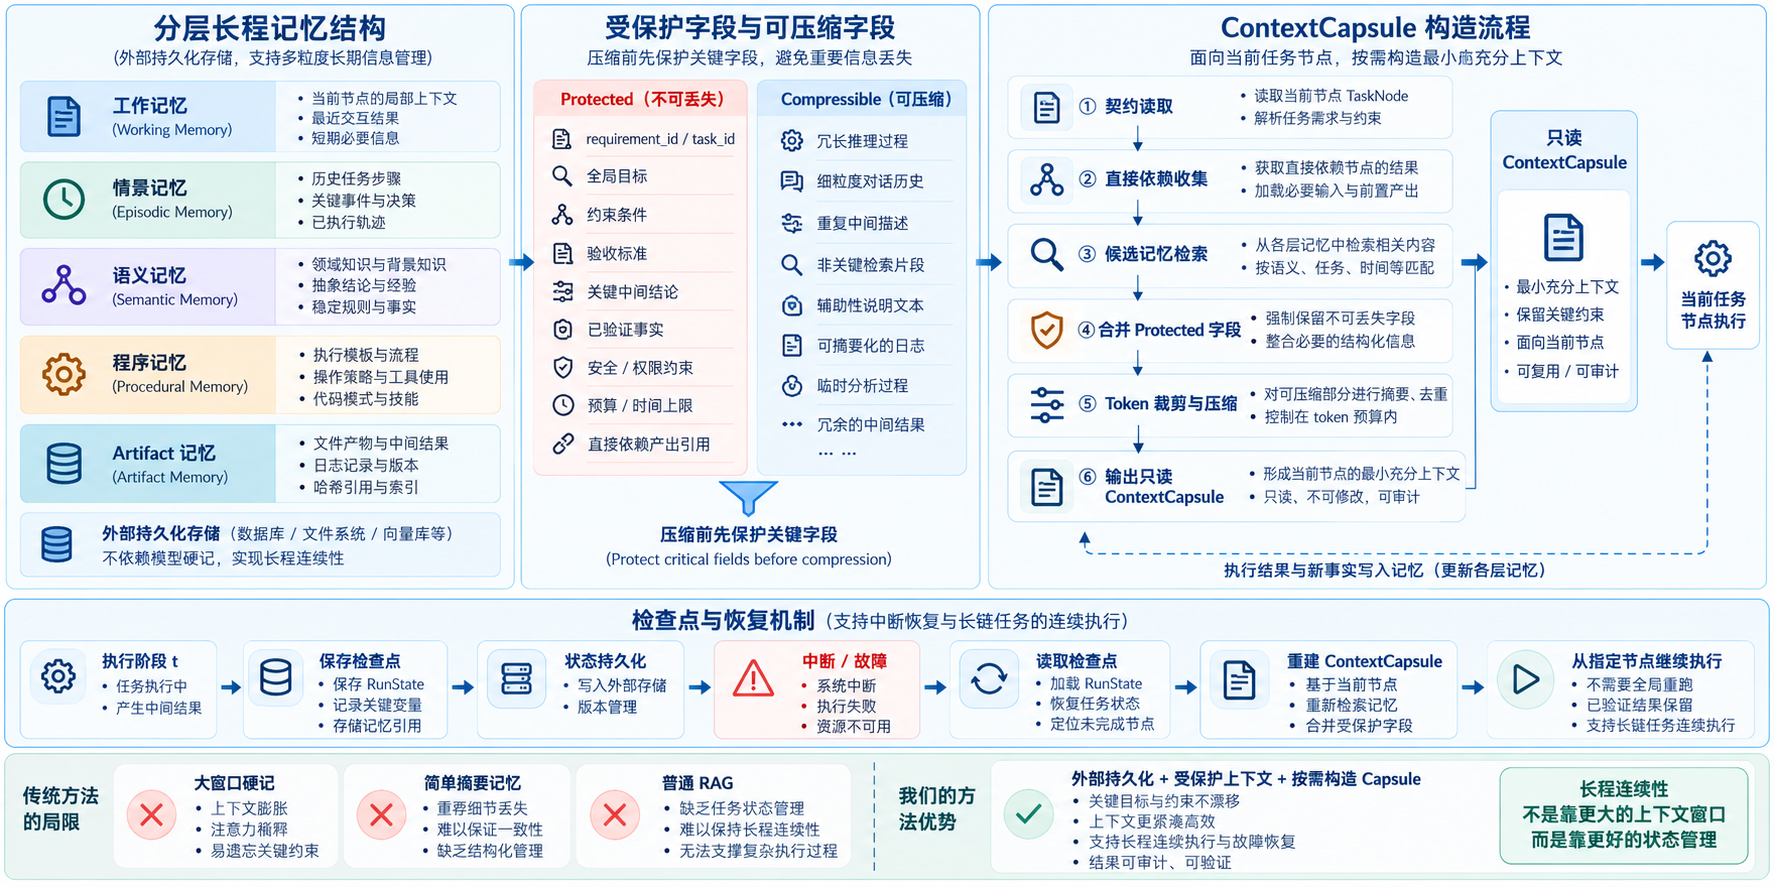
\includegraphics[width=0.98\textwidth]{figures/长程记忆与ContextCapsule上下文保持机制.png}
\caption{Dynamic-HMAS 长程状态与 ContextCapsule 机制：受保护状态、分层外部记忆、依赖检索、预算化上下文构造以及语义 checkpoint 共同维持长程任务连续性。}
\label{fig:memory-layers}
\end{figure}


\section{长程上下文的失效模式}

在数百至千步级 WorkUnit 的持续执行过程中，如果系统仅依赖模型上下文窗口保存历史信息，主要会出现五类失效模式。

第一类是\textbf{目标遗忘}。随着后续日志、模型输出和执行结果不断增加，早期任务目标、最终交付格式以及优化优先级可能逐渐退出有效上下文。

第二类是\textbf{约束漂移}。车辆尺寸、货物数量、金额上限、数据权限等硬约束如果与普通解释性文本一起反复摘要，可能被遗漏、改写或弱化。

第三类是\textbf{中间事实丢失}。后续节点可能无法准确判断哪些方案已经执行、哪些结果已经验证、哪些候选已经被否决，从而发生重复计算或使用过期结论。

第四类是\textbf{上下文膨胀}。如果每个节点都读取完整历史，则随着任务规模增长，输入 Token、延迟和无关信息会持续增加，并放大错误信息的传播范围。

第五类是\textbf{进程中断后的语义丢失}。普通模型上下文只存在于一次会话或调用过程中，进程重启后如果没有独立保存任务图、关键事实和验收状态，就只能从头重新构造任务语义。

因此，超长程任务的关键问题不是“模型窗口是否足够长”，而是以下状态是否能够跨节点、跨模型、跨资源和跨进程持续保持：
\[
\text{Goal}
+
\text{Constraints}
+
\text{Facts}
+
\text{Version}
+
\text{Evidence}
+
\text{Acceptance State}.
\]


\section{设计原则：从模型记忆到外部状态}

Dynamic-HMAS 将长程能力定义为：

\begin{quote}
任务中的关键状态能否在模型调用、节点执行、资源切换、图版本变化和进程中断之后继续保持一致，而不是单个模型能够在上下文窗口中容纳多少历史文本。
\end{quote}

基于这一原则，系统将长程信息划分为两类。

第一类是\textbf{任务正确性状态}，包括全局目标、硬约束、关键数量与金额、需求编号、图版本、artifact 来源、证据引用、验收状态和剩余重试预算。这些信息一旦丢失或被改写，可能直接改变任务结果，因此必须由控制面持久化并受到强制保护。

第二类是\textbf{辅助推理上下文}，包括解释性文本、普通分析过程、重复日志、低相关性历史以及可重新获取的信息。此类信息可以根据节点职责、语义相关性和 Token 预算进行检索、摘要、去重或外置。

因此，系统不要求每个 Agent 持有统一的完整历史，而是维护一个独立于模型生命周期的外部状态空间。模型只通过控制面构造的只读 ContextCapsule 获取执行当前任务所需的信息，不能直接修改全局记忆。

这种设计将长程连续性从模型内部不可验证的“记忆能力”，转化为控制面可以检查、恢复和审计的\textbf{状态连续性问题}。


\section{分层记忆与状态读写边界}

为区分不同信息的生命周期和访问方式，Dynamic-HMAS 将外部记忆划分为五类，如表~\ref{tab:memory-types} 所示。

\begin{longtable}{p{0.17\textwidth}p{0.41\textwidth}p{0.29\textwidth}}
\caption{Dynamic-HMAS 的分层记忆模型}
\label{tab:memory-types}\\
\toprule
类型 & 保存内容 & 主要用途\\
\midrule
\endfirsthead

\toprule
类型 & 保存内容 & 主要用途\\
\midrule
\endhead

工作记忆
& 当前节点输入、直接依赖结果、局部约束和错误上下文
& 支撑一次节点执行，完成后归档\\

情景记忆
& 节点事件、资源切换、需求变更、验证失败和修复尝试
& 重建时间顺序和异常恢复轨迹\\

语义记忆
& 全局目标、领域定义、已确认业务事实和稳定规则
& 跨阶段复用已经确认的任务知识\\

程序记忆
& 领域处理模板、执行命令、输出 Schema 和修复策略
& 复用可执行方法和流程约束\\

artifact 记忆
& 文件路径、来源节点、图版本、大小、哈希和摘要
& 通过引用复用大型对象，避免全文重复传输\\

\bottomrule
\end{longtable}

所有记忆由 Python 控制面写入持久化存储，并至少绑定
\texttt{task\_id}、
\texttt{node\_id}、
\texttt{graph\_version}、
\texttt{source\_node}
和
\texttt{content\_hash}。

Agent 不拥有全局记忆的直接写权限。节点执行后，控制面首先读取结构化输出和执行事件，再决定哪些信息可以进入长期状态。模型节点在下一次执行时只能读取由系统构造的只读 ContextCapsule。

因此，系统形成明确的读写边界：
\[
\begin{aligned}
&\text{Agent Output}
\rightarrow \text{Control-plane Validation} \\[3pt]
&\qquad\rightarrow \text{Persistent Memory}
\rightarrow \text{Read-only ContextCapsule}.
\end{aligned}
\]

这一边界避免模型直接将未经验证的推测写入长期事实空间。


\section{受保护状态不变量}

仅仅把信息写入外部数据库并不足以解决长程约束漂移问题。普通摘要算法仍然可能为了满足 Token 预算而删除影响任务正确性的关键字段。因此，Dynamic-HMAS 将上下文信息划分为
\textbf{protected}
和
\textbf{compressible}
两类。

受保护状态包括：

\begin{itemize}
    \item 全局任务目标；
    \item \texttt{requirement\_id} 及对应验收状态；
    \item 不可违反的业务硬约束；
    \item 关键数量、金额、阈值和几何参数；
    \item 输入文件和关键 artifact 路径；
    \item artifact 哈希及其来源节点；
    \item 当前任务图版本；
    \item 关键证据引用；
    \item 节点和需求验收状态；
    \item 剩余重试预算。
\end{itemize}

普通解释性文本、重复日志、低重要度讨论和可以重新检索的背景信息属于 compressible，可以摘要、去重、截断或外置。

对于任意待执行节点 $v$，设系统根据当前任务状态得到的受保护字段集合为
\[
P_v,
\]
最终构造的上下文胶囊为
\[
C_v.
\]

Dynamic-HMAS 要求始终满足以下\textbf{受保护状态完整性不变量}：
\[
P_v\subseteq C_v.
\]

即无论检索、摘要、压缩和 Token 裁剪如何发生，所有属于 $P_v$ 的关键状态都必须完整进入最终 ContextCapsule。

该约束的优先级高于普通上下文压缩。如果 Token 预算不足，系统首先减少 compressible 内容，而不能通过删除硬约束满足预算。若受保护状态本身已经超过当前节点允许的上下文预算，则系统应进入显式阻塞或重新调整执行策略，而不是静默丢弃正确性条件。

ContextCapsule 构造结束后，控制面执行完整性断言：
\[
containsAll(C_v,P_v)=true.
\]

只有完整性检查通过，当前节点才允许从 ready 状态进入 running。


\section{ContextCapsule 受约束构造机制}

ContextCapsule 的目标不是保存尽可能多的历史，而是在当前节点的上下文预算内，提供完成任务所需的\textbf{最小充分状态}。

对于节点 $v$，ContextCapsule 的信息来源主要包括三部分：

\[
C_v
=
P_v
\cup
D_v
\cup
R_v^{*},
\]

其中：

\begin{itemize}
    \item $P_v$ 为当前节点必须保留的 protected state；
    \item $D_v$ 为直接依赖节点的结构化输出；
    \item $R_v^{*}$ 为从普通外部记忆中选择的相关信息。
\end{itemize}

系统同时要求满足上下文预算约束：
\[
Tokens(C_v)\le B_v,
\]
其中 $B_v$ 表示节点 $v$ 的上下文 Token 预算。

由于 $P_v$ 具有不可删除性，因此预算优化只作用于普通候选记忆。设可检索的普通记忆集合为 $R_v$，则概念上可以将普通记忆选择表示为：
\[
R_v^{*}
=
\arg\max_{R'\subseteq R_v}
\sum_{m\in R'}score(m,v),
\]
满足：
\[
Tokens(P_v\cup D_v\cup R')\le B_v.
\]

该形式化说明 ContextCapsule 的目标并不是进行无约束的相似度检索，而是在受保护状态和 Token 预算两个硬条件下选择最有价值的普通上下文。


\subsection{普通记忆的唤醒排序}

对于普通可压缩记忆，系统综合考虑语义相关性、时间新近度、任务重要性、任务图距离以及事实是否具有可验证来源。

其排序关系可以抽象表示为：
\[
\begin{aligned}
score(m,v)
&= \alpha Rel(m,v) + \beta Recency(m) \\[3pt]
&\quad + \gamma Importance(m) + \delta Proximity(m,v) \\[3pt]
&\quad + \epsilon Evidence(m),
\end{aligned}
\]
其中：

\begin{itemize}
    \item $Rel(m,v)$ 表示记忆与当前任务节点的语义相关性；
    \item $Recency(m)$ 表示该信息在当前任务时间线上的新近程度；
    \item $Importance(m)$ 表示其对任务目标和验收结果的重要程度；
    \item $Proximity(m,v)$ 表示来源节点与当前节点在任务图中的结构距离；
    \item $Evidence(m)$ 表示该信息是否具有可信的 artifact 或验证来源。
\end{itemize}

需要强调的是，该评分只作用于普通可压缩记忆的排序，不参与 protected state 的保留决策。受保护字段无条件优先于普通检索结果。

上述公式用于描述当前记忆唤醒机制所考虑的排序因素，本文不将未经实验验证的具体权重取值表述为经过优化得到的最优参数。


\subsection{ContextCapsule 构造算法}

节点执行前，系统按照“契约—依赖—保护—检索—预算—完整性”的顺序构造上下文。

\begin{algorithm}[H]
\caption{受保护约束下的 ContextCapsule 构造}
\label{alg:context-capsule}
\KwIn{任务节点 $v$，全局记忆 $M_t$，图版本 $G_t$，Token 预算 $B_v$}
\KwOut{只读 ContextCapsule $C_v$ 或阻塞状态}

读取节点 $v$ 的 TaskNode 契约、职责和输出 Schema\;

$P_v \leftarrow$ 提取当前目标、硬约束、版本、验收状态和关键证据\;

$D_v \leftarrow$ 读取 $v$ 的直接依赖节点结构化结果\;

\If{$Tokens(P_v\cup D_v)>B_v$}{
    记录上下文预算不足并阻塞当前节点\;
}
\Else{
    $R_v \leftarrow$ 从语义、情景和程序记忆中检索普通候选\;

    按 $score(m,v)$ 对 $R_v$ 排序\;

    在剩余 Token 预算内选择 $R_v^{*}$\;

    $C_v \leftarrow P_v\cup D_v\cup R_v^{*}$\;

    计算 ContextCapsule 完整性哈希\;

    \If{$containsAll(C_v,P_v)=false$}{
        记录完整性失败并禁止节点进入 running\;
    }
    \Else{
        将 $C_v$ 冻结为只读上下文并交付节点\;
    }
}
\end{algorithm}

与普通历史摘要或单纯语义检索不同，ContextCapsule 同时具有三个核心性质。

\textbf{完整性（Completeness）}：
\[
P_v\subseteq C_v.
\]

\textbf{有界性（Boundedness）}：
\[
Tokens(C_v)\le B_v.
\]

\textbf{可追溯性（Traceability）}：
对于进入胶囊的关键事实 $x$，系统保存其来源信息
\[
Prov(x)
=
(source\_node,\ graph\_version,\ artifact\_hash).
\]

因此，ContextCapsule 不只是模型提示词的拼装结果，而是具有状态保护、预算约束和事实来源语义的运行时对象。


\section{ContextCapsule 数据结构与只读边界}

一个 ContextCapsule 的字段可以按照功能分为四类。

\begin{table}[htbp]
\centering
\caption{ContextCapsule 的主要字段分类}
\label{tab:capsule-fields}
\begin{tabularx}{0.96\textwidth}{p{0.22\textwidth}X}
\toprule
字段类别 & 主要内容\\
\midrule

身份与版本信息
&
\texttt{capsule\_id}、
\texttt{task\_id}、
\texttt{node\_id}、
\texttt{graph\_version}\\

受保护状态
&
\texttt{goal}、
\texttt{protected\_constraints}、
关键需求状态、
重试预算和关键业务事实\\

依赖与证据信息
&
\texttt{direct\_dependencies}、
\texttt{artifact\_refs}、
\texttt{evidence\_refs}、
来源节点和哈希\\

预算化辅助上下文
&
\texttt{relevant\_memories}、
\texttt{error\_context}、
\texttt{token\_budget}\\

完整性信息
&
\texttt{integrity\_hash}\\

\bottomrule
\end{tabularx}
\end{table}

其中，\texttt{goal} 和 \texttt{protected\_\allowbreak{}constraints} 用于防止目标和硬约束漂移；\texttt{direct\_\allowbreak{}dependencies} 保证节点优先使用直接上游事实；\texttt{artifact\_\allowbreak{}refs} 和 \texttt{evidence\_\allowbreak{}refs} 允许通过引用复用大型对象；\texttt{error\_\allowbreak{}context} 用于验证驱动修复；\texttt{integrity\_\allowbreak{}hash} 用于检测胶囊内容是否在交付节点后发生静默修改。

ContextCapsule 一旦构造完成，即作为只读对象交付模型或执行节点。节点可以基于胶囊内容产生候选结果，但不能直接修改胶囊中的全局目标、图版本和验收状态。


\section{记忆写入、版本管理与冲突裁决}

节点执行完成后，控制面从结构化输出、执行事件和验证结果中提取候选事实，并按照以下步骤写入长期状态：

\[
\begin{aligned}
&\text{Node Result}
\rightarrow \text{Source Binding}
\rightarrow \text{Version Binding} \\[3pt]
&\qquad\rightarrow \text{Hashing}
\rightarrow \text{Validation}
\rightarrow \text{Persistent Memory}.
\end{aligned}
\]

对于同一个事实的不同版本，系统不采用“最后一次写入覆盖旧值”的方式。旧值、新值、来源节点、图版本和触发事件均被保留，以防需求变更后的旧信息继续污染当前执行状态。

冲突裁决遵循以下优先级：

\begin{enumerate}
    \item 新任务图版本下通过验证的事实优先于旧图版本；
    \item 确定性验证结果优先于模型自报结果；
    \item 真实执行产生的结构化事实优先于间接自然语言转述；
    \item 直接依赖节点提供的信息优先于多级传播后的副本；
    \item 无法根据确定性规则消解的冲突进入显式 failed 或 blocked 状态。
\end{enumerate}

因此，长期记忆并不是无条件追加的聊天历史，而是具有来源、版本、有效性和验证状态的事实集合。


\section{语义 Checkpoint 与幂等恢复}

普通程序 checkpoint 通常只保存循环变量、模型参数或程序执行位置。对于 Dynamic-HMAS，这类信息不足以恢复超长程任务，因为系统还必须知道当前目标是什么、任务图处于哪个版本、哪些节点已经验证、哪些 artifact 仍然有效以及哪些需求已经闭合。

因此，本系统使用\textbf{语义 checkpoint} 保存完整运行语义。

在时刻 $t$，checkpoint 可以抽象表示为：
\[
K_t=
(
G_t,
M_t,
N_t,
A_t,
Q_t,
L_t,
B_t
),
\]
其中：

\begin{itemize}
    \item $G_t$ 表示当前任务图版本；
    \item $M_t$ 表示记忆快照；
    \item $N_t$ 表示节点状态及已完成节点集合；
    \item $A_t$ 表示 artifact manifest 及对应哈希；
    \item $Q_t$ 表示 Requirement Contract 的验收状态；
    \item $L_t$ 表示事件日志恢复位置；
    \item $B_t$ 表示剩余重试预算。
\end{itemize}

在具体实现中，每个 checkpoint 至少保存
\texttt{graph\_\allowbreak{}version}、
\texttt{completed\_\allowbreak{}nodes}、
\texttt{node\_\allowbreak{}status}、
\texttt{memory\_\allowbreak{}snapshot}、
\texttt{artifact\_\allowbreak{}manifest}、
\texttt{requirement\_\allowbreak{}digest}、
\texttt{event\_\allowbreak{}offset}
和
\texttt{retry\_\allowbreak{}budget}。

因此，系统恢复的不是简单的“执行到了第几步”，而是完整的\textbf{任务语义状态}。


\subsection{恢复一致性检查}

checkpoint 被重新载入后，系统首先验证快照自身和关键 artifact 的一致性。

恢复至少满足：

\[
Hash(K_t)=stored\_hash,
\]

并检查 checkpoint 中保存的
\texttt{requirement\_digest}
与当前恢复目标一致。

若 checkpoint 哈希损坏、需求摘要不一致或关键 artifact 无法通过哈希检查，则系统不能直接继续执行，而应进入显式错误处理流程。

通过一致性检查后，控制器恢复任务图、节点状态、记忆快照和 artifact manifest，并依据节点幂等键重建 ready 队列。已经验证的 WorkUnit 不重新执行，仅继续处理未完成或受到异常影响的节点。


\subsection{语义恢复算法}

\begin{algorithm}[H]
\caption{语义 Checkpoint 恢复与幂等重建}
\label{alg:semantic-checkpoint-recovery}
\KwIn{Checkpoint $K_t$，当前任务输入与需求摘要}
\KwOut{恢复后的运行状态或失败状态}

读取 checkpoint 元数据及完整性哈希\;

校验 $Hash(K_t)$ 与保存值是否一致\;

\If{checkpoint 完整性检查失败}{
    记录 checkpoint corruption 并停止恢复\;
}
\Else{
    校验 \texttt{requirement\_digest} 是否与当前恢复目标一致\;

    \If{需求摘要不一致}{
        进入需求变更处理流程，不直接复用旧状态\;
    }
    \Else{
        恢复任务图版本和节点状态\;

        恢复 memory snapshot 与 artifact manifest\;

        校验关键 artifact 的路径和哈希\;

        根据事件偏移恢复运行日志位置\;

        根据幂等键跳过已验证 WorkUnit\;

        重建剩余 ready 队列\;

        从未完成或受影响节点继续执行\;
    }
}
\end{algorithm}

该机制使恢复过程具有幂等性：同一个已经验证完成的 WorkUnit 不会因为进程重新实例化而再次执行。


\section{长程连续性的评价指标}

为了避免仅凭主观描述说明“系统记住了任务”，Dynamic-HMAS 使用机器可读指标评价状态连续性。

\subsection{关键字段保持率}

设当前任务共有 $N_{critical}$ 个必须保留的关键字段，恢复或长程执行结束后仍然保持正确的字段数量为 $N_{kept}$，则：

\[
Retention
=
\frac{N_{kept}}{N_{critical}}.
\]

该指标主要衡量全局目标、硬约束、关键数值、图版本和证据引用是否发生丢失或漂移。

历史运行 \texttt{20260903\_160722} 的末端 ContextCapsule 保留全部 12 个预定义关键字段，即：
\[
Retention=\frac{12}{12}=1.
\]

\subsection{恢复重复率}

为了检验 checkpoint 恢复是否发生重复执行，定义：

\[
ReplayRate
=
\frac{N_{duplicate}}{N_{unit}},
\]

其中 $N_{duplicate}$ 表示恢复后被错误重复执行的已验证 WorkUnit 数量，$N_{unit}$ 表示总 WorkUnit 数量。

当前两项千步级实验中均记录：
\[
N_{duplicate}=0.
\]

\subsection{版本一致性与完整性}

系统进一步检查以下指标：

\begin{itemize}
    \item 节点使用的 \texttt{graph\_version} 是否与当前运行状态一致；
    \item ContextCapsule 是否通过 protected state 完整性检查；
    \item checkpoint 哈希是否一致；
    \item artifact 引用及哈希是否有效；
    \item 恢复前后的 \texttt{requirement\_digest} 是否一致。
\end{itemize}

这些指标共同用于判断系统是否真正恢复了任务状态，而不仅是重新启动了程序。


\section{千步级恢复证据}

在城市多模态真实数据千步运行中，系统将 1,000 个 WorkUnit 按固定间隔写入 checkpoint，共形成 40 个快照。运行在第 500 步重新实例化，并从 checkpoint 20 恢复。

恢复过程中，控制面重新加载任务图版本、memory snapshot、artifact manifest、需求摘要和已完成 WorkUnit 集合，随后重建 ready 队列。已经验证的前 500 个单元根据幂等键被跳过，最终重复执行数量为 0。

MathorCup 千步候选优化实验同样保存 40 个 checkpoint，并按照相同的状态恢复机制管理已经完成的候选评估。

这些实验不能证明系统具有“无限长度记忆”，但能够直接证明当前实现中的 checkpoint 并非只保存程序计数器，而是能够恢复图、记忆、artifact 和需求状态共同构成的任务语义。


\section{ContextCapsule 的对照评价设计}

为了进一步区分 ContextCapsule 与普通历史摘要机制，本章将长程上下文方法的比较重点定义为以下几个维度：

\begin{itemize}
    \item \textbf{关键字段保持率}：硬约束、目标和关键状态是否能够长期保持；
    \item \textbf{平均输入上下文}：每次模型调用实际需要输入的 Token 数量；
    \item \textbf{约束漂移}：长期摘要后关键约束是否出现遗漏或改变；
    \item \textbf{恢复一致性}：中断后是否能够保持图版本和已验证事实；
    \item \textbf{最终任务成功}：完整业务、证据和需求门禁是否通过。
\end{itemize}

一个完整的控制变量实验可以比较 Full History、Summary Only 和 ContextCapsule 三种策略，如表~\ref{tab:memory-ablation-design} 所示。

\begin{table}[htbp]
\centering
\caption{长程上下文机制的控制变量评价设计}
\label{tab:memory-ablation-design}
\begin{tabularx}{0.96\textwidth}{p{0.20\textwidth}X X X}
\toprule
方法
& 关键字段保持
& 上下文控制方式
& 状态恢复语义\\
\midrule

Full History
& 不显式保护
& 注入全部历史
& 依赖额外状态机制\\

Summary Only
& 依赖摘要质量
& 递归摘要历史
& 可能丢失被摘要信息\\

ContextCapsule
& Protected invariant
& 保护字段 + 直接依赖 + 预算检索
& 图、记忆、artifact 与需求联合恢复\\

\bottomrule
\end{tabularx}
\end{table}

当前报告仅使用已经产生的真实运行结果说明 ContextCapsule 的关键字段保持率和 checkpoint 恢复能力，不对尚未完成同等条件实测的 Full History 或 Summary Only 策略虚构 Token、成功率或约束漂移数据。若后续完成统一模型、统一输入和统一预算下的控制实验，再在第七章更新定量结果。


\section{跨场景状态实例}

不同领域需要长期保持的具体事实不同，但都遵循同一套 protected state、ContextCapsule 和 checkpoint 语义。表~\ref{tab:cross-domain-memory} 给出了三个代表性场景。

\begin{table}[htbp]
\centering
\caption{不同任务场景中的长程状态实例}
\label{tab:cross-domain-memory}
\begin{tabularx}{0.96\textwidth}{p{0.19\textwidth}X X}
\toprule
场景
& 需要长期保护的关键状态
& 可压缩或外置的信息\\
\midrule

MathorCup 装箱
&
车辆尺寸、货物类型和数量、重量、易碎规则、顶部间隙、成本目标、已验证 placements
&
普通方案解释、重复运行日志、低价值候选分析\\

差旅报销
&
费用金额、日期、票据来源、政策约束、异常原因、验收状态
&
重复政策解释、普通分析过程和中间描述\\

城市多模态
&
不同数据源的统计范围、来源哈希、隐私边界、图版本及已确认跨模态事实
&
大型原始文本、重复记录及可通过引用访问的原始数据\\

\bottomrule
\end{tabularx}
\end{table}

三个场景中的业务字段差异明显，但系统并不为每个领域重新设计一套记忆系统。变化的是 protected state 的具体内容和领域验证规则，不变的是状态分类、ContextCapsule 构造、来源绑定、版本管理和 checkpoint 恢复机制。


\section{本章小结}

本章将超长程任务中的“记忆问题”重新定义为一个由确定性控制面管理的\textbf{状态连续性问题}。

Dynamic-HMAS 首先将影响任务正确性的目标、硬约束、关键事实、图版本、证据和验收状态从普通模型上下文中分离出来，并通过 protected invariant 保证：
\[
P_v\subseteq C_v.
\]
由此，关键状态不会为了满足摘要或 Token 截断而被静默删除。

在此基础上，ContextCapsule 依据当前节点契约，将 protected state、直接依赖结果和相关外部记忆组合为预算有界的最小充分上下文，并同时满足完整性、有界性和事实可追溯性。模型只能读取胶囊而不能直接修改全局状态，从而将开放式推理与长期事实存储相互隔离。

语义 checkpoint 则进一步将任务图、节点状态、memory snapshot、artifact manifest、需求摘要和重试预算共同持久化，使进程中断后恢复的是完整任务语义，而不仅是程序执行位置。当前真实运行中，末端 ContextCapsule 保持 12/12 个关键字段；城市多模态真实数据千步实验在第 500 步从 checkpoint 20 恢复，40 个 checkpoint 完整保留，已验证 WorkUnit 重复执行数量为 0。

因此，Dynamic-HMAS 的长程能力并不依赖单模型的超长上下文窗口，而是通过\textbf{受保护外部状态、预算化 ContextCapsule 和语义 checkpoint}，把“长期记住任务”转化为一个可以被检查、恢复和审计的系统状态连续性机制。后续章节将在该状态基础上进一步讨论异构资源路由以及验证驱动的可信执行与自主修复。


\chapter{端边云协同与语义保持式异构资源路由}

本章研究 Dynamic-HMAS 在异构模型与执行资源条件下的任务调度问题。
复杂任务中的不同 TaskNode 在语义复杂度、数据敏感性、实时性、
计算需求和结果质量要求方面存在显著差异，因此，将所有节点固定发送到
同一种模型或同一执行位置，既不能充分利用异构资源，也可能违反数据位置、
安全等级和时延等硬性约束。

Dynamic-HMAS 的端边云协同并非简单地在多个模型端点之间选择一个进行调用，
而是将\textbf{资源选择纳入版本化任务状态}。
系统以契约化 TaskNode 为最小路由单位，根据能力、安全、数据位置、
实时性和预算形成节点资源需求画像；
首先执行不可被其他指标补偿的硬约束过滤，再在合法候选资源之间综合质量、
时延、成本、历史可靠性和负载进行软评分排序。
当当前资源发生运行级故障时，控制面只迁移执行后端，
而保持 TaskSpec、任务图版本、Protected Context、
已经验证的 artifact 和 Requirement 状态不变。

因此，本章重点解决的并不是简单的“应该调用哪个模型”，而是：

\begin{quote}
在执行资源动态变化的情况下，如何选择合法且合适的端、边、云资源，
并保证资源迁移不会破坏长程任务的语义、事实状态和可信执行链。
\end{quote}

围绕这一目标，本章形成
\textbf{TaskNode 需求驱动路由、不可补偿硬约束、语义保持式资源回退和可审计路由来源链}
四项相互关联的机制。

\begin{figure}[htbp]
\centering
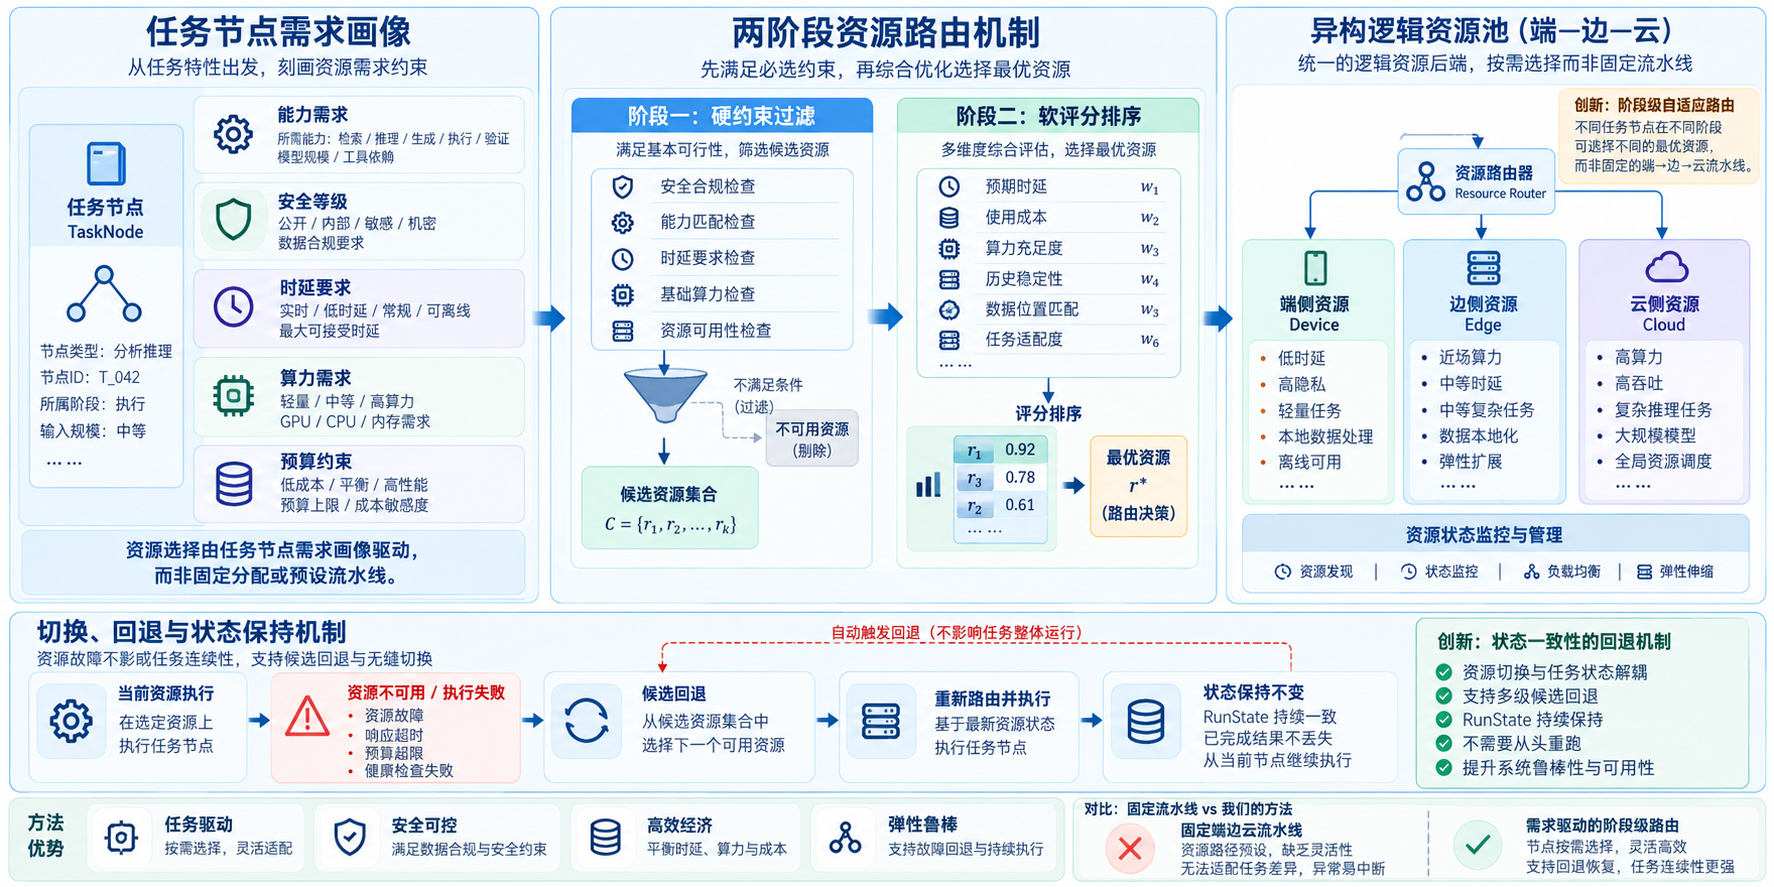
\includegraphics[width=0.98\textwidth]{figures/端边云协同与阶段级资源路由机制.png}
\caption{Dynamic-HMAS 端边云协同与语义保持式资源路由机制：TaskNode 首先形成资源需求画像，经过不可补偿硬约束过滤和合法候选软排序选择逻辑端、边、云资源；资源级失败后保持任务语义并执行可审计回退。}
\label{fig:device-edge-cloud-routing}
\end{figure}


\section{问题定义与设计目标}

设时刻 $t$ 系统已经注册的资源集合为
\[
\mathcal{R}_t=
\{r_1,r_2,\ldots,r_m\}.
\]

对于当前待执行任务节点 $v$，系统需要选择资源
\[
r_v^{*}\in\mathcal{R}_t,
\]
使其首先满足能力、安全、位置、算力和可用性等不可违反条件，
随后再在合法资源之间优化质量、时延、成本和运行稳定性。

因此，Dynamic-HMAS 将资源路由抽象为：
\[
r_v^{*}
=
Route
\left(
d_v,
\mathcal{R}_t,
\sigma_t
\right),
\]
其中：

\begin{itemize}
    \item $d_v$ 表示 TaskNode $v$ 的资源需求画像；
    \item $\mathcal{R}_t$ 表示当前 ResourceRegistry 中的运行时资源状态；
    \item $\sigma_t$ 表示当前任务状态；
    \item $r_v^{*}$ 表示最终选择的执行资源。
\end{itemize}

当前全局状态仍沿用全文统一表示：
\[
\sigma_t=(G_t,M_t,A_t,Q_t),
\]
其中 $G_t$ 为任务图版本，$M_t$ 为记忆状态，
$A_t$ 为带来源和哈希的 artifact 集合，
$Q_t$ 为需求验收账本。

资源路由需要遵循以下四项基本原则。

\begin{enumerate}
    \item \textbf{合法性优先于性能偏好。}
    不满足能力、安全、数据位置等硬约束的资源不得进入候选集合，
    无论其模型能力、成本或响应速度多么有优势。

    \item \textbf{TaskNode 而非 Agent 是最小路由单位。}
    同一个 Planner、Analyst 或 Code Generator
    在处理不同节点时可能具有不同的安全、实时性和质量需求，
    因此不存在固定的 Agent--Model 绑定关系。

    \item \textbf{资源变化不得改变任务语义。}
    fallback 只允许改变实际执行后端，
    不得静默修改任务目标、图版本、关键约束、
    已验证 artifact 和需求验收状态。

    \item \textbf{路由过程必须可追踪。}
    系统需要保存候选资源、淘汰原因、评分、最终选择、
    fallback 过程和实际执行结果，以支持后续审计。
\end{enumerate}


\section{逻辑端边云资源模型}

当前 Dynamic-HMAS 中的 device、edge 和 cloud 表示
\textbf{逻辑资源位置}，用于刻画不同执行资源的能力、
数据位置、安全条件和运行特征。

单个资源描述符定义为：
\[
r=
(
id,
loc,
model,
cap,
comp,
lat,
cost,
sec,
avail,
conc,
load,
hist
),
\]
其中：

\begin{itemize}
    \item $id$：资源唯一标识；
    \item $loc$：逻辑位置，
    $loc\in\{device,edge,cloud\}$；
    \item $model$：资源绑定的模型、工具或执行后端；
    \item $cap$：资源支持的能力集合；
    \item $comp$：计算能力或任务复杂度承载等级；
    \item $lat$：历史或当前延迟特征；
    \item $cost$：资源调用或执行的相对成本；
    \item $sec$：可满足的数据安全和访问等级；
    \item $avail$：当前可用状态；
    \item $conc$：并发容量；
    \item $load$：当前负载；
    \item $hist$：历史成功率、失败情况及运行可靠性。
\end{itemize}

ResourceRegistry 负责维护这些描述符的静态能力信息和动态运行状态。
资源调用成功、超时、连接失败、主动下线或连续发生错误后，
对应的可用性、失败记录和历史可靠性均可被更新，
并参与后续节点的资源选择。

\begin{table}[htbp]
\centering
\caption{逻辑端、边、云资源的职责差异}
\label{tab:logical-device-edge-cloud}
\begin{tabularx}{0.96\textwidth}{p{0.17\textwidth}X X}
\toprule
逻辑位置 & 主要特征 & 典型适用任务\\
\midrule

端侧 Device
&
靠近数据源，可优先满足数据本地性和低外传需求，
适合稳定的本地程序和工具执行
&
文件解析、哈希计算、格式转换、本地工具、
确定性预处理及允许条件下的轻量模型任务
\\

边侧 Edge
&
在数据位置、模型能力和响应时延之间提供折中
&
中等复杂度分析、低时延推理、
局部数据处理和阶段性模型任务
\\

云侧 Cloud
&
通常提供更高模型能力和更丰富的计算资源，
但受到网络、成本和数据策略限制
&
全局规划、复杂分析、代码候选生成和
安全策略允许的高复杂度语义推理
\\

\bottomrule
\end{tabularx}
\end{table}

需要强调的是，表~\ref{tab:logical-device-edge-cloud}
描述的是资源层的逻辑职责，而不是固定角色绑定。
实际执行位置仍由当前 TaskNode 的需求和 ResourceRegistry 的运行状态决定。


\section{TaskNode 需求驱动的资源画像}

传统静态多 Agent 系统常将某一种 Agent 永久绑定到一个固定模型。
例如 Planner 始终使用大型云模型，Retriever 始终使用某个本地模型。
这种方式无法处理同一角色在不同任务阶段中的资源需求变化。

Dynamic-HMAS 将资源需求绑定到 TaskNode 而非 Agent 类型。

对于节点 $v$，定义资源需求画像：
\[
d_v=
(
cap_v,
sec_v,
loc_v,
comp_v,
lat_v,
quality_v,
budget_v
),
\]
其中：

\begin{itemize}
    \item $cap_v$：节点必须具备的能力集合；
    \item $sec_v$：任务和输入数据的安全等级；
    \item $loc_v$：允许的逻辑执行位置；
    \item $comp_v$：最低计算或模型能力需求；
    \item $lat_v$：最大允许延迟或实时性要求；
    \item $quality_v$：结果质量要求；
    \item $budget_v$：Token、成本或其他资源预算。
\end{itemize}

因此，系统不存在：
\[
AgentRole
\Rightarrow
FixedResource,
\]
而采用：
\[
TaskNodeDemand
+
RuntimeState
\Rightarrow
ResourceSelection.
\]

即使两个节点均属于 Analyst，
当一个节点处理公开文本而另一个节点处理受限数据时，
二者可以因为 $sec_v$ 和 $loc_v$ 不同而获得完全不同的候选资源集合。

这一机制使资源调度能够真正随任务语义和运行环境动态变化，
而不是仅根据智能体名称预先配置模型。


\section{不可补偿硬约束与合法候选生成}

Dynamic-HMAS 将资源选择划分为两个阶段：

\[
\boxed{
\text{Legality First}
\rightarrow
\text{Preference Second}
}
\]

第一阶段不进行性能权衡，而只回答一个问题：

\begin{quote}
当前资源是否具有执行该 TaskNode 的合法资格？
\end{quote}

对于节点 $v$，定义时刻 $t$ 的合法资源集合：
\[
\mathcal{C}_v(t)
=
\left\{
r\in\mathcal{R}_t
\mid
H(r,v,t)=true
\right\},
\]
其中硬约束函数可以展开为：
\[
\begin{aligned}
H(r,v,t)
&= CapabilityOK(r,v) \land SecurityOK(r,v) \\[3pt]
&\quad {}\land LocationOK(r,v) \land Available(r,t) \\[3pt]
&\quad {}\land ComputeOK(r,v) \land ConcurrencyOK(r,t).
\end{aligned}
\]

如果时延属于当前节点不可违反的条件，还需满足：
\[
Latency(r,t)\leq LatencyLimit(v).
\]

因此：
\[
\mathcal{C}_v(t)
=
\left\{
r\in\mathcal{R}_t
\mid
H(r,v,t)=true
\right\}.
\]

这一设计的关键在于：
\textbf{硬约束不可补偿（Non-compensable Hard Constraints）}。

例如，如果某资源不满足任务的数据安全等级，
则即使它具有更高模型质量、更低费用和更小时延，
也不会因为综合评分更高而重新进入候选集合。

换言之，本系统不采用：
\[
Score
=
Security
+
Quality
+
Cost
+
Latency
\]
这种可能使安全劣势被其他优势抵消的单阶段加权方式，
而是首先形成合法集合，再执行偏好排序。

如果：
\[
\mathcal{C}_v(t)=\varnothing,
\]
控制器不会为了完成任务而自动放宽安全、能力或位置限制，
而是将节点置为 waiting、blocked 或进入显式资源恢复流程。


\section{合法资源的软评分排序}

硬过滤完成后，剩余资源已经全部满足不可违反条件。
第二阶段只在合法资源之间比较质量、成本和运行特征。

\subsection{连续指标归一化}

由于质量、成本、时延、失败率和负载的量纲不同，
直接将原始数值相加缺乏可比性。

对于连续型指标 $x$，在当前合法候选集合中执行归一化：
\[
\hat{x}(r)
=
\frac{x(r)-x_{\min}}
{x_{\max}-x_{\min}+\varepsilon},
\]
其中 $\varepsilon$ 为避免分母为零的微小常数。

归一化仅用于合法资源之间的相对排序，
不会改变上一节的硬约束判断结果。


\subsection{运行状态感知的综合评分}

对于合法候选 $r\in\mathcal{C}_v(t)$，
定义资源评分：
\[
\begin{aligned}
Score(r,v,t)
&= w_q\hat{Q}(r,v) + w_h\hat{Hist}(r,t) \\[3pt]
&\quad {}- w_c\hat{Cost}(r,v) - w_l\hat{Latency}(r,t) \\[3pt]
&\quad {}- w_f\hat{Failure}(r,t) - w_u\hat{Load}(r,t),
\end{aligned}
\]
其中：

\begin{itemize}
    \item $\hat{Q}(r,v)$：资源与当前节点能力和质量要求的匹配程度；
    \item $\hat{Hist}(r,t)$：历史成功和稳定性表现；
    \item $\hat{Cost}(r,v)$：预计调用或运行成本；
    \item $\hat{Latency}(r,t)$：当前或历史时延；
    \item $\hat{Failure}(r,t)$：近期失败和连续失败程度；
    \item $\hat{Load}(r,t)$：当前资源负载。
\end{itemize}

各权重满足：
\[
w_q,w_h,w_c,w_l,w_f,w_u\geq0.
\]

最终选择：
\[
r_v^{*}
=
\arg\max_{r\in\mathcal{C}_v(t)}
Score(r,v,t).
\]

本文不将未经统一实验优化的某一组具体权重描述为理论最优参数。
该评分函数的主要作用是在\textbf{合法候选内部}进行运行时偏好排序，
而不是通过调节权重改变硬约束。

因此，资源路由整体可以表示为：
\[
r_v^{*}
=
\arg\max_{r\in\mathcal{R}_t}
Score(r,v,t),
\]
subject to
\[
H(r,v,t)=true.
\]


\section{TaskNode 级阶段式多模型协同}

本文所述端边云协同属于
\textbf{TaskNode 级阶段式多模型路由}，
而不是 Transformer 参数层级的模型切分。

复杂任务首先由动态任务图分解为：
\[
G_t=(V_t,E_t),
\]
对于：
\[
V_t=
\{v_1,v_2,\ldots,v_n\},
\]
每个节点分别执行：
\[
r_{v_i}^{*}
=
Route(d_{v_i},\mathcal{R}_t,\sigma_t).
\]

最终形成：
\[
\{
v_1\rightarrow r_{v_1}^{*},
v_2\rightarrow r_{v_2}^{*},
\ldots,
v_n\rightarrow r_{v_n}^{*}
\}.
\]

因此，异构资源协同发生在任务阶段和节点级。

不同节点可以使用不同模型或工具，
但下游节点并不需要了解上游实际运行在 device、edge 还是 cloud，
而只依据标准化 TaskNode 输出契约消费结果。

这种解耦使：
\[
ExecutionBackend
\]
可以变化，而：
\[
TaskSemantics
\]
保持稳定。

例如，一个复杂任务中可以出现：

\begin{itemize}
    \item 数据格式检查和哈希计算由靠近数据源的确定性资源完成；
    \item 对实时性敏感的中等复杂度节点由逻辑边侧资源执行；
    \item 高复杂度规划和代码候选生成在安全条件允许时由能力较强的逻辑云资源完成；
    \item 领域验证节点由能够读取真实 artifact 并稳定复算的执行后端完成。
\end{itemize}

上述只是运行时可能形成的资源分工，
并非预先写死的 Agent--Model 配置。


\section{语义保持式资源迁移与故障回退}

本章最关键的设计并不是“资源失败以后换一个模型”，
而是保证：

\begin{quote}
资源可以变化，但任务语义和已经确认的事实不能随资源一起变化。
\end{quote}

本文将这一机制称为：
\textbf{语义保持式资源迁移}
（Semantic-Preserving Resource Migration）。


\subsection{资源级失败与任务级失败}

系统首先区分两种不同故障。

\textbf{资源级失败}包括：

\begin{itemize}
    \item 模型服务连接失败；
    \item 调用超时；
    \item 当前资源不可用；
    \item 并发或容量不足；
    \item 执行环境异常；
    \item 明确属于执行后端的运行故障。
\end{itemize}

资源级失败主要触发：
\[
ResourceFailure
\rightarrow
ResourceUpdate
\rightarrow
ReRoute.
\]

\textbf{任务级失败}则包括：

\begin{itemize}
    \item Schema 错误；
    \item 业务约束违反；
    \item 代码逻辑错误；
    \item 结果不完整；
    \item 证据无法闭合。
\end{itemize}

任务级失败进入第六章介绍的：
\[
ValidationError
\rightarrow
Attribution
\rightarrow
AffectedSubgraph
\rightarrow
Repair.
\]

因此，不会因为结果本身错误就盲目更换模型；
也不会因为资源暂时不可用就重新解释整个用户任务。


\subsection{资源迁移状态不变量}

对于节点 $v$，定义执行前需要保持的关键任务状态：
\[
S_v=
(
TaskSpec,
G_t,
C_v,
A_t^{verified},
Q_t,
B_t
),
\]
其中：

\begin{itemize}
    \item $G_t$ 为当前图版本；
    \item $C_v$ 为节点只读 ContextCapsule；
    \item $A_t^{verified}$ 为已经验证的事实与 artifact；
    \item $Q_t$ 为 Requirement Contract 验收状态；
    \item $B_t$ 为剩余执行和重试预算。
\end{itemize}

当节点从资源 $r_i$ 切换到 $r_j$ 时，
系统要求以下核心语义保持不变量：

\[
TaskSpec'=TaskSpec,
\]

\[
G_t'=G_t,
\]

\[
Protected(C_v')=Protected(C_v),
\]

\[
A_t^{verified'}=A_t^{verified},
\]

\[
Q_t'=Q_t.
\]

换言之，fallback 允许修改的是：
\[
resource\_id,
\quad
model,
\quad
route\_record,
\quad
execution\_record,
\]
而不能修改已经确认的任务事实。

重试预算可以按照运行策略正常减少，
但不能因为换了一个资源就重新获得无限预算。

因此，资源回退的系统语义不是：
\[
\text{``重新开始任务''},
\]
而是：
\[
\text{``保持任务状态，迁移执行位置''}.
\]


\section{可审计的路由来源链}

普通模型路由器通常只输出最终的模型或 endpoint。
Dynamic-HMAS 则将\textbf{路由决策本身视为一种运行事实}，
并保存完整 RouteRecord。

一个 RouteRecord 至少包括：

\begin{itemize}
    \item \texttt{task\_id}；
    \item \texttt{node\_id}；
    \item \texttt{graph\_version}；
    \item 当前 TaskNode demand profile；
    \item 当前 ResourceRegistry 快照或候选摘要；
    \item 被硬约束过滤的资源；
    \item 每个淘汰资源的过滤原因；
    \item 合法候选集合；
    \item 候选评分；
    \item 最终 \texttt{resource\_id}；
    \item 实际模型或执行后端；
    \item 是否发生 fallback；
    \item fallback 原因；
    \item 实际执行结果。
\end{itemize}

由此，一次路由过程能够形成：
\[
\begin{aligned}
&Demand \rightarrow Candidates \rightarrow HardFilter
\rightarrow LegalCandidates \\[3pt]
&\qquad\rightarrow Scores \rightarrow SelectedResource
\rightarrow Execution.
\end{aligned}
\]

评审者可以进一步回答：

\begin{itemize}
    \item 为什么某个资源没有进入候选集合；
    \item 当前资源为什么被选择；
    \item 是否存在安全限制被绕过；
    \item 资源失败后系统为什么选择某个备用资源；
    \item fallback 后是否仍使用相同任务图和 protected state。
\end{itemize}

因此，Resource Routing 不再只是控制面内部无法解释的瞬时决策，
而成为与节点状态、artifact 和最终验收结果共同保存的
\textbf{可审计运行 provenance}。


\section{端边云路由的系统级创新}

Dynamic-HMAS 的阶段级异构资源调度并不以单次调用价格最低
或单一模型质量最高作为唯一目标，
而是同时维护资源合法性、任务语义连续性和路由决策可追溯性。

其系统级创新主要体现在以下四个方面。

\subsection{从 Agent 绑定转向 TaskNode-aware Routing}

资源选择不由智能体名称直接决定，
而是由当前节点契约和运行状态共同决定：
\[
r_v^{*}
=
Route(d_v,\mathcal{R}_t,\sigma_t).
\]

因此，同一个 Agent 角色可以在不同节点选择不同模型或资源，
不同 Agent 也可以因为任务需求相同而共享同一个合法资源。

这种设计使资源拓扑能够随着任务图变化而同步变化。


\subsection{不可补偿的合法性优先机制}

能力、安全、位置和数据边界首先形成：
\[
\mathcal{C}_v(t),
\]
软评分只允许发生在：
\[
r\in\mathcal{C}_v(t).
\]

因此，质量优势和成本优势无法“买掉”安全限制，
资源调度具有显式的安全边界。


\subsection{语义保持式 Fallback}

资源故障不重新解释任务，
而是在：
\[
TaskSpec,\ G_t,\ Protected(C_v),\ A_t^{verified},\ Q_t
\]
保持一致的情况下替换执行后端。

因此，fallback 是执行位置迁移，
而不是任务状态重置。


\subsection{路由 provenance 与可信执行链融合}

RouteRecord 与：
\[
node\_id,
\quad
graph\_version,
\quad
artifact,
\quad
ValidationResult
\]
共同进入机器可读运行状态。

资源选择能够与最终结果建立因果联系，
而不是在执行结束后无法解释某个结果究竟由哪个模型和资源产生。

因此，本章机制可以概括为：
\[
\boxed{
\begin{aligned}
&\text{TaskNode-aware Routing}
+ \text{Non-compensable Constraints} \\[3pt]
&\quad {}+ \text{Semantic-preserving Fallback}
+ \text{Auditable Provenance}
\end{aligned}
}
\]

这也是 Dynamic-HMAS 端边云协同区别于静态角色绑定
和单纯多模型 endpoint 选择的核心所在。


\section{异构资源路由算法}

算法~\ref{alg:heterogeneous-resource-routing}
给出完整的 TaskNode 级异构资源选择与回退过程。

% 仅收紧本算法的字号与行距，保持完整伪代码在单页正文区域内。
\begingroup
\small
\setstretch{1.1}
\begin{algorithm}[H]
\caption{任务语义保持的阶段级异构资源路由}
\label{alg:heterogeneous-resource-routing}

\KwIn{
任务节点 $v$，
当前资源集合 $\mathcal{R}_t$，
系统状态 $\sigma_t$
}
\KwOut{
执行资源 $r_v^{*}$ 或 waiting/blocked 状态
}

$d_v\leftarrow buildDemandProfile(v,\sigma_t)$\;

$\mathcal{C}_v\leftarrow\varnothing$\;

\ForEach{$r\in\mathcal{R}_t$}{
    \eIf{
        $CapabilityOK(r,v)$ 且
        $SecurityOK(r,v)$ 且
        $LocationOK(r,v)$ 且
        $Available(r,t)$ 且
        $ComputeOK(r,v)$ 且
        $ConcurrencyOK(r,t)$
    }{
        将 $r$ 加入 $\mathcal{C}_v$\;
    }{
        记录 $r$ 的硬约束淘汰原因\;
    }
}

\If{$\mathcal{C}_v=\varnothing$}{
    记录 no legal resource\;
    将节点置为 waiting 或 blocked\;
    \Return no-resource\;
}

对 $\mathcal{C}_v$ 中连续指标执行归一化\;

\ForEach{$r\in\mathcal{C}_v$}{
    $s_r\leftarrow Score(r,v,t)$\;
}

按 $s_r$ 从高到低形成合法候选队列 $\mathcal{Q}_v$\;

保存当前 TaskSpec、图版本、Protected Context、
已验证 artifact 和需求状态\;

\While{$\mathcal{Q}_v\neq\varnothing$ 且 retry budget $>0$}{
    $r\leftarrow popBest(\mathcal{Q}_v)$\;

    写入 RouteRecord\;

    $result\leftarrow execute(v,r)$\;

    \eIf{$result.success$}{
        更新资源成功历史\;
        保存 execution record\;
        \Return $r$\;
    }{
        \eIf{$result$ 属于资源级失败}{
            更新资源失败率、可用性和连续失败记录\;
            扣减资源重试预算\;
            验证任务语义保持不变量\;
            继续选择下一合法候选\;
        }{
            将执行结果交给确定性验证与 Repair 路径\;
            \Return $r$\;
        }
    }
}

写入 failed 或 blocked 状态\;

\end{algorithm}
\endgroup

该算法具有两个重要性质。

第一，无论执行多少次 fallback，
安全、位置和能力硬约束都不会被自动放宽。

第二，只有明确属于资源层的失败才触发候选资源切换；
如果执行本身成功但业务结果错误，则进入 Validation-driven Repair，
而不是简单换一个模型再次生成。


\section{复杂度分析}

设 ResourceRegistry 中当前共有 $C$ 个资源。

硬约束过滤需要对资源集合进行一次遍历，因此：
\[
T_{filter}=O(C).
\]

设通过过滤后的合法资源数量为：
\[
C'\leq C.
\]

对合法候选计算评分需要：
\[
O(C').
\]

若需要得到完整排序，则复杂度为：
\[
O(C'\log C').
\]

因此，单个 TaskNode 的最坏资源选择复杂度为：
\[
O(C\log C).
\]

候选资源列表、评分和 RouteRecord 所需空间最多为：
\[
O(C).
\]

如果只需要得到单个最高分资源，
可以在线性扫描过程中保留当前最大值，
将第一次选择降低为：
\[
O(C).
\]

但当前路由逻辑保留候选排序信息，
便于资源失败后按顺序 fallback，
同时为路由审计保存完整候选依据。

需要说明的是，上述复杂度只描述控制面的资源过滤和排序，
不包含实际模型推理、网络通信或外部工具运行时间。


\section{可验证路由指标}

为了避免将“系统可以调用多个模型”直接等同于“实现了端边云协同”，
本文为异构资源路由定义机器可统计指标。


\subsection{路由合法率}

定义：
\[
RoutingLegalRate
=
\frac{N_{legal}}
{N_{route}},
\]
其中 $N_{route}$ 表示全部实际路由决策，
$N_{legal}$ 表示最终选择同时满足全部硬约束的路由数量。

该指标检查系统是否曾经选择不具备合法执行资格的资源。


\subsection{故障回退成功率}

定义：
\[
FallbackSuccessRate
=
\frac{N_{fallback\_success}}
{N_{fallback}}.
\]

只有在原资源发生明确资源级失败后，
备用资源完成实际执行并重新进入正常验证流程，
才计为一次成功 fallback。


\subsection{安全违规次数}

定义：
\[
SecurityViolation
=
N_{\text{illegal-security-route}}.
\]

由于安全等级属于不可补偿硬约束，
系统的目标值为：
\[
SecurityViolation=0.
\]


\subsection{路由可追溯率}

若一次路由能够完整恢复：
\[
\begin{aligned}
&Demand \rightarrow CandidateResources \rightarrow FilterReason \\[3pt]
&\qquad\rightarrow Score \rightarrow SelectedResource
\rightarrow Execution,
\end{aligned}
\]
则认为该路由记录可追踪。

定义：
\[
RouteTraceabilityRate
=
\frac{N_{traceable}}
{N_{route}}.
\]


\subsection{其他运行指标}

运行日志还可以统计：

\begin{itemize}
    \item Model Distribution；
    \item Logical Location Distribution；
    \item Average Latency；
    \item 不同 TaskNode 类型的资源使用分布；
    \item fallback 次数；
    \item 连续资源失败次数；
    \item 单资源历史成功情况。
\end{itemize}

上述指标均应由机器可读 RouteRecord 和 execution record 统计。
若当前运行数据尚未完成统一汇总，
本文不填入未经统计验证的百分比结果。


\section{跨场景资源协同实例}

端边云路由机制本身不依赖具体业务场景。
不同领域主要改变 TaskNode 的资源需求画像，
而 ResourceRegistry、合法性过滤、评分、fallback 和 RouteRecord 保持一致。

\begin{table}[htbp]
\centering
\caption{不同场景中的资源需求差异}
\label{tab:cross-domain-resource-demand}
\begin{tabularx}{0.97\textwidth}{p{0.20\textwidth}X X}
\toprule
场景或阶段 & 主要资源需求 & 复用的控制机制\\
\midrule

MathorCup 代码生成
&
较强代码生成能力、允许的模型资源、明确预算
&
TaskNode demand、Hard Filter、Soft Ranking
\\

MathorCup 真实执行
&
本地文件读写、Python 执行环境和稳定的 artifact 输出
&
ResourceDescriptor、ExecutionRecord
\\

差旅报销文件处理
&
数据权限、文件解析能力和确定性金额计算
&
安全过滤、资源合法性判断
\\

差旅政策分析
&
文本理解能力、政策上下文和结果质量要求
&
节点级模型路由和 RouteRecord
\\

城市多模态来源处理
&
数据位置、来源边界、吞吐和确定性处理能力
&
位置约束、能力过滤、状态保持
\\

全局综合分析
&
较高语义推理能力和已经验证的结构化输入
&
质量排序、ContextCapsule、可审计调用
\\

\bottomrule
\end{tabularx}
\end{table}

由此，新场景不需要重新设计路由器，
只需为新的 TaskNode 声明资源约束，
并通过 ResourceRegistry 注册合法执行资源。


\section{与长程状态和可信执行的协同关系}

端边云路由并非独立于其他章节存在。

首先，它依赖第四章的 ContextCapsule。
无论 TaskNode 最终被路由到哪一个资源，
模型或执行器读取的任务语义均来自同一只读胶囊。
因此，资源后端变化不会导致节点重新从完整聊天历史解释任务。

其次，它与第六章的可信执行共享事实边界。
资源路由决定：
\[
\text{Where to Execute},
\]
而 Terminal Executor、Domain Validator 和 Evidence Verifier 决定：
\[
\text{Whether the Result is Valid}.
\]

资源质量分数再高，也不能替代真实执行和业务验证。

最后，路由与 Validation-driven Repair 执行不同类型的恢复：

\[
ResourceFailure
\rightarrow
ReRoute,
\]
而：
\[
BusinessFailure
\rightarrow
Repair.
\]

这一分离避免资源恢复、业务修复和任务重新规划彼此混淆，
也使系统能够根据故障来源选择最小必要恢复动作。


\section{实现边界与能力说明}

为保证端边云部分的表述与当前实现一致，
本章明确以下能力边界。

\begin{enumerate}
    \item \textbf{当前 device、edge、cloud 为逻辑资源位置。}
    它们用于抽象资源能力、安全和执行位置，
    并不等价于已经部署真实物理边缘集群。

    \item \textbf{当前实现属于阶段级多模型路由。}
    系统按照 TaskNode 选择不同模型或执行后端，
    不涉及 Transformer 参数层切分、tensor parallel、
    pipeline parallel 或同一模型参数跨端边云协同。

    \item \textbf{本章验证重点是控制语义而非物理网络性能。}
    当前系统重点验证资源合法性过滤、运行时选择、
    fallback 和路由可追踪性，
    不将其表述为真实边缘网络吞吐或分布式 GPU 性能测试。

    \item \textbf{安全约束不会因资源故障自动放宽。}
    当不存在合法备用资源时，
    系统应进入 waiting、blocked 或 failed，
    而不是自动将敏感任务迁移到不合法位置。

    \item \textbf{兼容性结论限于已接入接口。}
    当前系统通过 OpenAI-compatible 模型接口和
    ResourceDescriptor 支持逻辑异构资源，
    但不据此宣称任意模型和硬件均能够零适配接入。
\end{enumerate}

因此，当前 Dynamic-HMAS 的“端边云协同”更准确地定义为：

\begin{quote}
面向契约化 TaskNode 的逻辑端、边、云异构资源自适应路由，
以及在任务语义不变条件下的状态保持式故障迁移。
\end{quote}


\section{本章小结}

本章建立了 Dynamic-HMAS 的端边云协同与语义保持式异构资源路由机制。

系统没有将 Planner、Analyst 等 Agent 永久绑定到固定模型，
而是以 TaskNode 为最小资源调度单位，
根据能力、安全、位置、实时性、计算需求和预算构造节点需求画像：
\[
d_v=
(
cap_v,
sec_v,
loc_v,
comp_v,
lat_v,
quality_v,
budget_v
).
\]

在资源选择过程中，
系统首先通过不可补偿硬约束形成合法候选集合：
\[
\mathcal{C}_v(t)
=
\left\{
r\in\mathcal{R}_t
\mid
H(r,v,t)=true
\right\},
\]
随后只在合法资源之间执行运行状态感知的软评分：
\[
r_v^{*}
=
\arg\max_{r\in\mathcal{C}_v(t)}
Score(r,v,t).
\]

该机制的核心并不是单纯采用“硬过滤 + 软排序”，
而是进一步形成四项系统能力：
\[
\boxed{
\begin{aligned}
&\text{TaskNode-aware Routing}
+ \text{Non-compensable Constraints} \\[3pt]
&\quad {}+ \text{Semantic-preserving Fallback}
+ \text{Auditable Provenance}
\end{aligned}
}.
\]

其中，TaskNode-aware Routing 使资源选择随节点任务语义变化；
不可补偿约束保证安全、能力和位置要求不会被性能优势抵消；
语义保持式 fallback 保证执行资源变化时
TaskSpec、图版本、Protected Context、
已经验证的 artifact 和需求状态保持一致；
RouteRecord 则将资源选择本身转化为可复核的运行事实。

因此，Dynamic-HMAS 中资源可以动态变化，
但任务目标、可信事实和验收语义不会随资源迁移而漂移。
这种设计使端边云协同真正进入统一确定性控制面，
并与动态图、ContextCapsule、真实执行和 Validation-driven Repair
共同构成长程自治任务的完整运行闭环。

需要再次说明的是，
当前系统实现的是逻辑端、边、云资源后端以及
TaskNode 级阶段式多模型路由，
并不涉及 Transformer 参数层切分或真实物理多机边缘集群。
后续第六章将进一步讨论路由后的候选结果如何通过真实执行、
确定性验证和证据闭合转化为可信事实，
第七章则在当前能力边界内给出多场景运行和路由故障恢复的实验依据。

\chapter{可信执行、证据闭合与验证驱动自主修复}

本章研究 Dynamic-HMAS 如何将大模型产生的开放式候选结果转化为可以被系统接受的可信交付结果。对于复杂任务，模型能够生成格式合理的文本、JSON、代码和方案，但“生成结果”并不等价于“业务事实成立”。代码可能无法真实执行，结构化输出可能违反领域约束，报告中的声明也可能缺少对应执行产物。因此，如果系统允许模型依据自身输出直接判断任务成功，就可能产生“语言上完成、业务上错误”的假成功。

Dynamic-HMAS 的核心设计是不要求模型自证正确，而是建立一条由确定性控制面管理的\textbf{执行锚定可信链}。模型输出首先被视为 Candidate；只有经过真实执行后才能形成 Observable Fact；进一步通过确定性领域验证和证据核验后，才能升级为 Verified Fact；最终还必须满足 Requirement Contract 和 Final Gate，才具有 Deliverable Fact 的交付资格。

当验证失败时，系统同样不将失败简单转换为“再次调用一次模型”，而是把验证结果结构化为可执行的控制信号，沿 artifact 来源定位责任节点，计算受影响子图，并将具体错误、领域约束和剩余预算注入 RepairContext，重新生成、真实执行并再次完成全部验收。由此形成“生成—执行—验证—归因—修复—再验证”的闭环。

\begin{figure}[htbp]
\centering
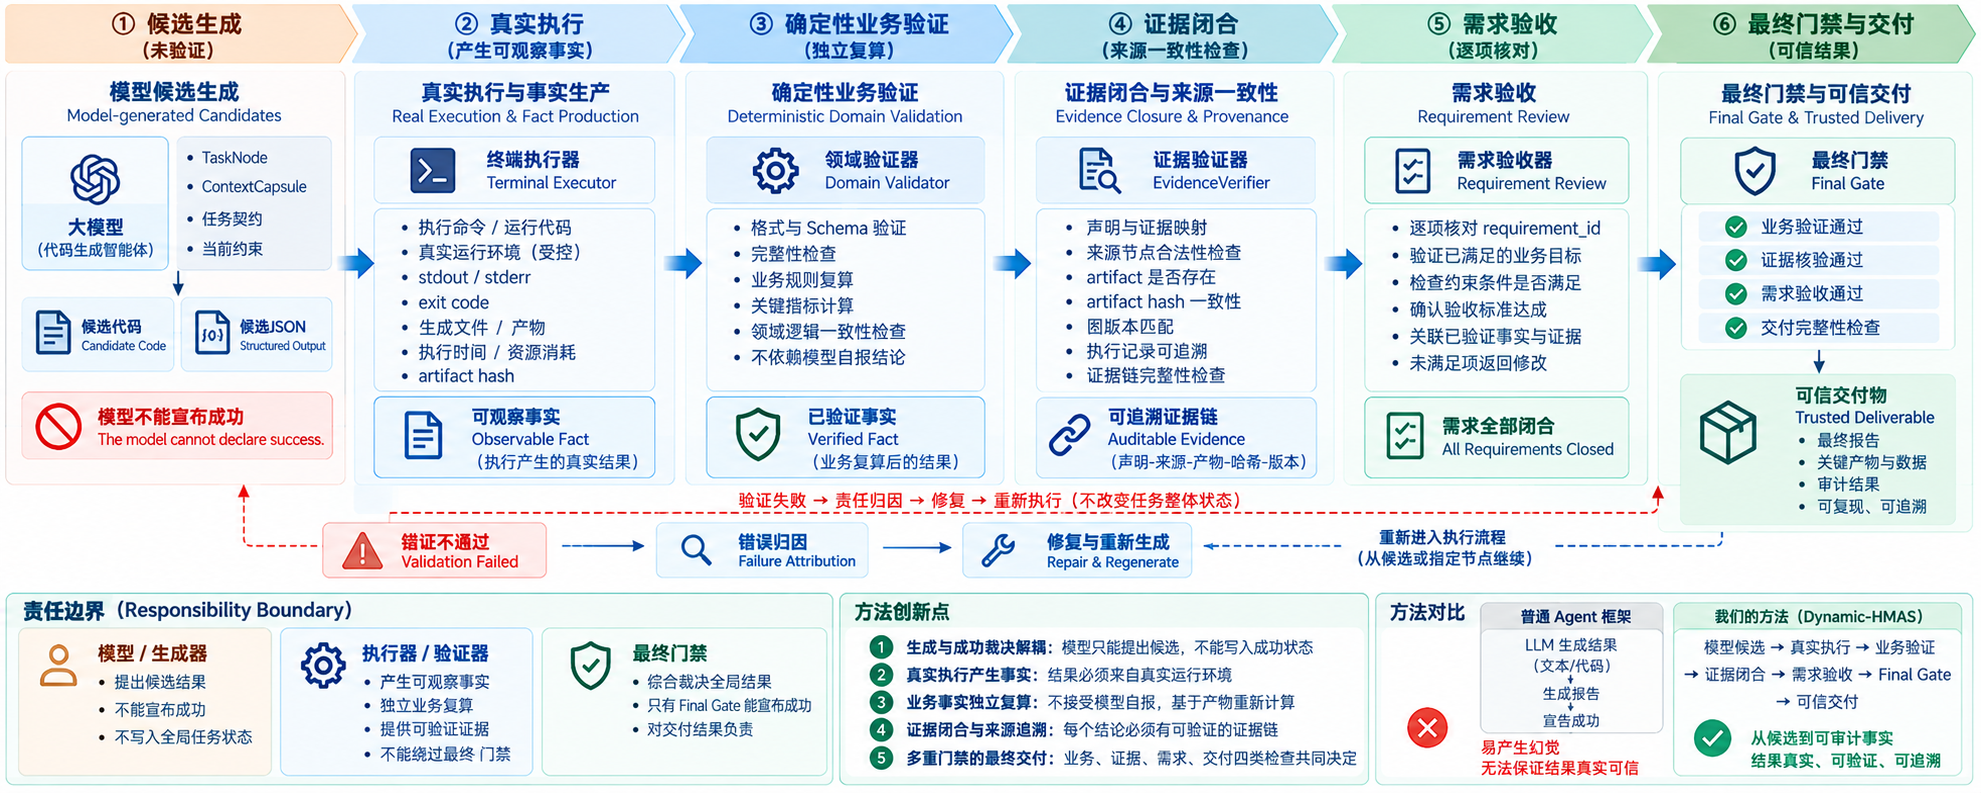
\includegraphics[width=0.98\textwidth]{figures/可信执行、证据闭合与最终交付门禁.png}
\caption{Dynamic-HMAS 的可信事实形成与交付链：模型候选必须经过真实执行、领域验证、证据闭合、需求验收和最终门禁后，才能进入可信交付状态。}
\label{fig:trust-loop}
\end{figure}


\section{可信执行问题与设计原则}

开放域智能体系统面临的关键问题并不是模型“能否生成一个答案”，而是系统如何判断这个答案是否真的成立。Dynamic-HMAS 将可信执行中的风险归纳为四类。

\begin{table}[htbp]
\centering
\caption{可信执行中的主要风险与控制机制}
\label{tab:trusted-execution-risks}
\begin{tabularx}{0.96\textwidth}{p{0.20\textwidth}X X}
\toprule
风险类型 & 典型表现 & 主要控制机制\\
\midrule

候选生成风险
&
代码无法运行、JSON Schema 错误、计算逻辑错误、模型误报约束满足
&
真实终端执行、Schema 检查、确定性领域验证\\

状态一致性风险
&
旧结果覆盖新结果、artifact 与图版本不一致、需求变更后继续使用旧事实
&
图版本绑定、artifact 哈希、状态机和幂等键\\

证据可信风险
&
关键声明无实际来源、路径错误、文件不存在、哈希不一致
&
Evidence Verifier、producer 绑定和版本化证据闭合\\

修复过程风险
&
只修改验证状态、复用旧结果、跳过真实执行或无限重复调用
&
RepairContext、强制重新执行、重试预算和 Final Gate\\

\bottomrule
\end{tabularx}
\end{table}

针对上述风险，系统遵循四项设计原则。

\begin{enumerate}
    \item \textbf{模型输出默认不是事实。}
    模型产生的代码、文本和结构化结果首先只能进入候选状态。

    \item \textbf{事实必须锚定真实执行。}
    只有 Terminal Executor 实际执行后产生的进程状态、文件和 artifact，才能形成可观察事实。

    \item \textbf{业务正确性与证据真实性分开验证。}
    Domain Validator 回答“结果在业务上是否正确”，Evidence Verifier 回答“该结果是否确实来自本次运行中的合法来源”。

    \item \textbf{错误必须改变后续控制状态。}
    ValidationResult 不只是记录“通过或失败”，还要驱动责任归因、局部图重开和修复执行。
\end{enumerate}

因此，系统不仅具备“完成任务”的能力，也具备在条件不足、验证失败或证据不闭合时\textbf{拒绝错误交付}的能力。


\section{从候选到可信交付的事实状态跃迁}

Dynamic-HMAS 将任务结果划分为四种不同可信等级：

\[
\text{Candidate}
\rightarrow
\text{Observable Fact}
\rightarrow
\text{Verified Fact}
\rightarrow
\text{Deliverable Fact}.
\]

这种划分用于明确区分“模型说了什么”“系统实际发生了什么”“结果是否正确”以及“是否允许最终交付”。

\subsection{候选状态：Candidate}

对于任务节点 $v$，模型根据当前 ContextCapsule 产生候选结果：
\[
c_v = Generate(C_v),
\]
其中 $c_v$ 可以是自然语言结论、结构化 JSON、代码、运行参数或修复方案。

Candidate 可以参与后续执行，但其内容不能直接写入全局事实状态，也不能修改最终 \texttt{outcome}。

例如，Code Generator 可以输出一段声称“满足全部装箱约束”的程序，但在真实运行和确定性验证之前，这一声明仍然只是候选。


\subsection{可观察事实：Observable Fact}

Terminal Executor 将候选结果转化为实际系统行为：
\[
o_v = Execute(c_v).
\]

执行过程中记录：

\begin{itemize}
    \item 实际执行命令；
    \item 标准输出与标准错误；
    \item 退出码；
    \item 执行时间；
    \item 生成文件列表；
    \item artifact 路径；
    \item artifact 哈希；
    \item 对应 producer node 和图版本。
\end{itemize}

只有此时，系统才能确认“某段代码实际运行过”“某个文件实际产生过”。因此，Terminal Executor 产生的是\textbf{可观察事实}，但这些事实仍然可能违反业务规则。


\subsection{已验证事实：Verified Fact}

对于可观察结果 $o_v$，领域验证器执行：
\[
z_v = Validate(o_v).
\]

当且仅当业务约束和证据来源均满足时，该结果才被升级为 Verified Fact：
\[
Verified(o_v)
=
BusinessValid(o_v)
\land
EvidenceValid(o_v).
\]

其中，BusinessValid 用于确认结构、数量、几何、金额、成本等领域条件；EvidenceValid 用于确认结果的 producer、artifact、图版本和哈希来源合法。


\subsection{可交付事实：Deliverable Fact}

即使一个结果已经通过局部业务和证据验证，也不意味着整个用户需求已经完成。最终进入报告和交付结果的事实还必须满足 Requirement Contract。

定义：
\[
Deliverable(x)
=
Verified(x)
\land
RequirementAccepted(x)
\land
VersionConsistent(x).
\]

最终交付链可以表示为：
\[
\begin{aligned}
&\text{Model Generation}
\rightarrow \text{Terminal Execution}
\rightarrow \text{Domain Validation} \\[3pt]
&\qquad\rightarrow \text{Evidence Verification}
\rightarrow \text{Requirement Acceptance}
\rightarrow \text{Final Gate}.
\end{aligned}
\]

这一事实状态跃迁机制使“生成结果”和“任务成功”成为两个严格分离的概念。


\section{受控真实执行与事实生产}

Code Generator 和 Terminal Executor 在系统中承担不同职责。

Code Generator 根据 TaskNode 契约产生候选代码、运行参数和执行建议，但不拥有文件系统事实和全局状态的最终写权限。Terminal Executor 则在受控运行环境中创建代码文件、执行命令，并捕获实际运行结果。

一次执行至少记录：
\[
ExecutionRecord=
(command,exit\_code,stdout,stderr,time,files,hash).
\]

所有执行结果与以下信息绑定：
\[
(task\_id,node\_id,graph\_version,resource\_id).
\]

这种分离使模型无法通过自然语言声称“程序已经执行成功”来替代真实进程结果。即使候选代码在文本上看起来正确，只要实际执行失败，节点就不会进入已验证状态。

同时，Terminal Executor 产生的 artifact 被记录对应的 \texttt{producer\_node}，为后续验证错误的责任归因提供稳定来源。


\section{确定性领域验证}

Domain Validator 的职责是从实际 artifact 中重新计算业务事实，而不是接受生成模型对结果的自我评价。

为了避免 Domain Validator 与 Evidence Verifier 的职责重叠，本文将领域确定性验证划分为四层。

\subsection{结构合法性验证}

第一层检查结构化结果是否能够被系统正确解析，包括：

\begin{itemize}
    \item JSON 或其他结构格式是否合法；
    \item 必填字段是否存在；
    \item 字段类型是否正确；
    \item 枚举值是否属于允许集合；
    \item 数值是否满足基本范围要求。
\end{itemize}


\subsection{结果完整性验证}

第二层检查任务对象是否完整覆盖，包括：

\begin{itemize}
    \item 输入对象是否全部得到处理；
    \item 是否存在漏项；
    \item 是否存在重复项；
    \item 是否出现未知类型或非法记录；
    \item 输出文件是否满足规定数量和格式。
\end{itemize}


\subsection{领域约束验证}

第三层检查特定领域规则。

以 MathorCup 装箱任务为例，验证内容包括：

\begin{itemize}
    \item 货物坐标是否位于车辆边界内；
    \item 旋转后的尺寸是否满足空间限制；
    \item 三维 AABB 是否发生非法重叠；
    \item 易碎件堆叠规则是否满足；
    \item 顶部间隙是否满足；
    \item 车辆重量是否超过限制。
\end{itemize}

在差旅报销等其他场景中，该层可以替换为金额、日期、票据和政策规则。


\subsection{运营指标复算}

第四层独立计算最终业务指标。

MathorCup 结果契约包含：

\begin{itemize}
    \item \texttt{vehicle\_scenarios}；
    \item \texttt{multi\_vehicle\_scenarios}；
    \item \texttt{placements}；
    \item \texttt{vehicle\_count}；
    \item \texttt{total\_cost}；
    \item \texttt{space\_utilization\_rate}；
    \item \texttt{load\_utilization\_rate}；
    \item \texttt{validation}。
\end{itemize}

其中，\texttt{vehicle\_count} 和 \texttt{total\_cost} 不接受模型提供的最终数值作为事实，而是由领域验证器根据实际 placements、车辆分配和成本规则重新计算。

因此，模型即使输出：
\[
vehicle\_count=5,\qquad total\_cost=3500,
\]
系统仍需要依据实际结果独立复算后才能接受这两个字段。

该机制直接防止坐标越界、货物数量不完整、利用率异常或成本字段错误被“格式正确的 JSON”掩盖。


\section{版本化证据闭合与事实来源链}

业务正确并不等于证据可信。为了防止报告中的关键声明脱离实际运行产物，系统为每项关键声明建立版本化证据对象：
\[
e=
(
claim,
source\_node,
artifact,
graph\_version,
hash
).
\]

其中：

\begin{itemize}
    \item $claim$ 表示需要被支撑的关键结论；
    \item $source\_node$ 表示直接生产相关事实的节点；
    \item $artifact$ 表示实际运行文件；
    \item $graph\_version$ 表示该事实对应的任务图版本；
    \item $hash$ 表示 artifact 内容完整性哈希。
\end{itemize}

对于证据对象 $e$，系统要求：
\[
\begin{aligned}
EvidenceClosed(e)
&= Exists(artifact) \\[3pt]
&\quad \land HashMatch(artifact) \\[3pt]
&\quad \land VersionMatch(artifact,G_t) \\[3pt]
&\quad \land ProducerMatch(artifact,source\_node).
\end{aligned}
\]

Evidence Verifier 主要检查：

\begin{itemize}
    \item artifact 是否实际存在；
    \item 文件哈希是否一致；
    \item producer node 是否与声明来源一致；
    \item artifact 是否来自正确图版本；
    \item 关键结果是否具有真实 Terminal Execution 记录；
    \item 声明是否仅依赖允许的直接证据来源。
\end{itemize}

运行目录中的证据路径可以包括：

\begin{itemize}
    \item \texttt{artifacts/result.json}；
    \item \texttt{artifacts/tool\_results/terminal\_execution/terminal\_execution.json}；
    \item \texttt{artifacts/result\_complete.json}；
    \item \texttt{artifacts/constraint\_validation\_log.json}；
    \item \texttt{artifacts/cost\_comparison.json}。
\end{itemize}

证据闭合不是最终报告生成后的附加检查，而是进入交付阶段之前的硬门禁。如果文件不存在、哈希不匹配、producer 不一致或图版本错误，即使模型已经生成语言上完整的报告，该结果仍然不能成为 Deliverable Fact。


\section{结构化 ValidationError 与责任归因}

Dynamic-HMAS 不把验证失败简单表示为一个布尔值，而是将其结构化为可被控制面直接消费的错误对象。

定义：
\[
err=
(
type,
field,
index,
expected,
actual,
artifact,
owner,
severity
).
\]

其中：

\begin{itemize}
    \item $type$ 表示错误类别；
    \item $field$ 表示发生错误的字段；
    \item $index$ 表示错误对象位置；
    \item $expected$ 表示预期条件或合法范围；
    \item $actual$ 表示实际结果；
    \item $artifact$ 表示发生错误的结果文件；
    \item $owner$ 表示责任节点；
    \item $severity$ 表示错误严重程度。
\end{itemize}

常见错误包括：

\begin{itemize}
    \item Schema 错误；
    \item 编译错误；
    \item 进程错误；
    \item 边界越界；
    \item AABB 重叠；
    \item 数量不匹配；
    \item 易碎件堆叠错误；
    \item 重量超限；
    \item 成本不一致；
    \item 证据缺失；
    \item 需求未闭合。
\end{itemize}

系统根据 artifact 的 \texttt{producer\_node}、实际执行日志和验证规则完成责任归因：
\[
O=
Attribute(err,Provenance),
\]
其中 $O$ 表示责任节点集合。

例如，当
\[
\texttt{placements[11].x}
\]
超出车辆允许边界时，错误记录保留字段、索引、允许范围和实际值，并通过 result artifact 的 producer 将责任定位到生成该 placement 的代码节点。

若业务结果本身正确，但缺少成本比较 artifact，则责任不会被错误地归因到装箱算法，而应落在证据生成或验收链路。


\subsection{错误严重程度与控制动作}

系统将错误分为四级：

\begin{table}[htbp]
\centering
\caption{验证错误等级与主要处理动作}
\label{tab:error-severity}
\begin{tabularx}{0.96\textwidth}{p{0.14\textwidth}p{0.42\textwidth}X}
\toprule
等级 & 典型情况 & 主要动作\\
\midrule

Level 1
& 不影响业务正确性的提示或非关键问题
& 记录并允许流程继续\\

Level 2
& 可通过重新生成实现修复的领域业务错误
& 定位责任节点并执行 Repair\\

Level 3
& 编译失败、进程失败、资源执行错误
& 重新生成、重新执行或资源切换\\

Level 4
& 输入缺失、无合法资源、安全约束无法满足或预算耗尽
& 进入 blocked 或 failed，不允许假成功\\

\bottomrule
\end{tabularx}
\end{table}

这种分类避免系统将所有失败统一处理为“再次调用模型”，也避免把不可恢复的安全和资源问题进入无限重试。


\section{受影响子图与验证驱动自主修复}

图~\ref{fig:repair-loop} 展示验证失败后的控制路径。

\begin{figure}[htbp]
\centering
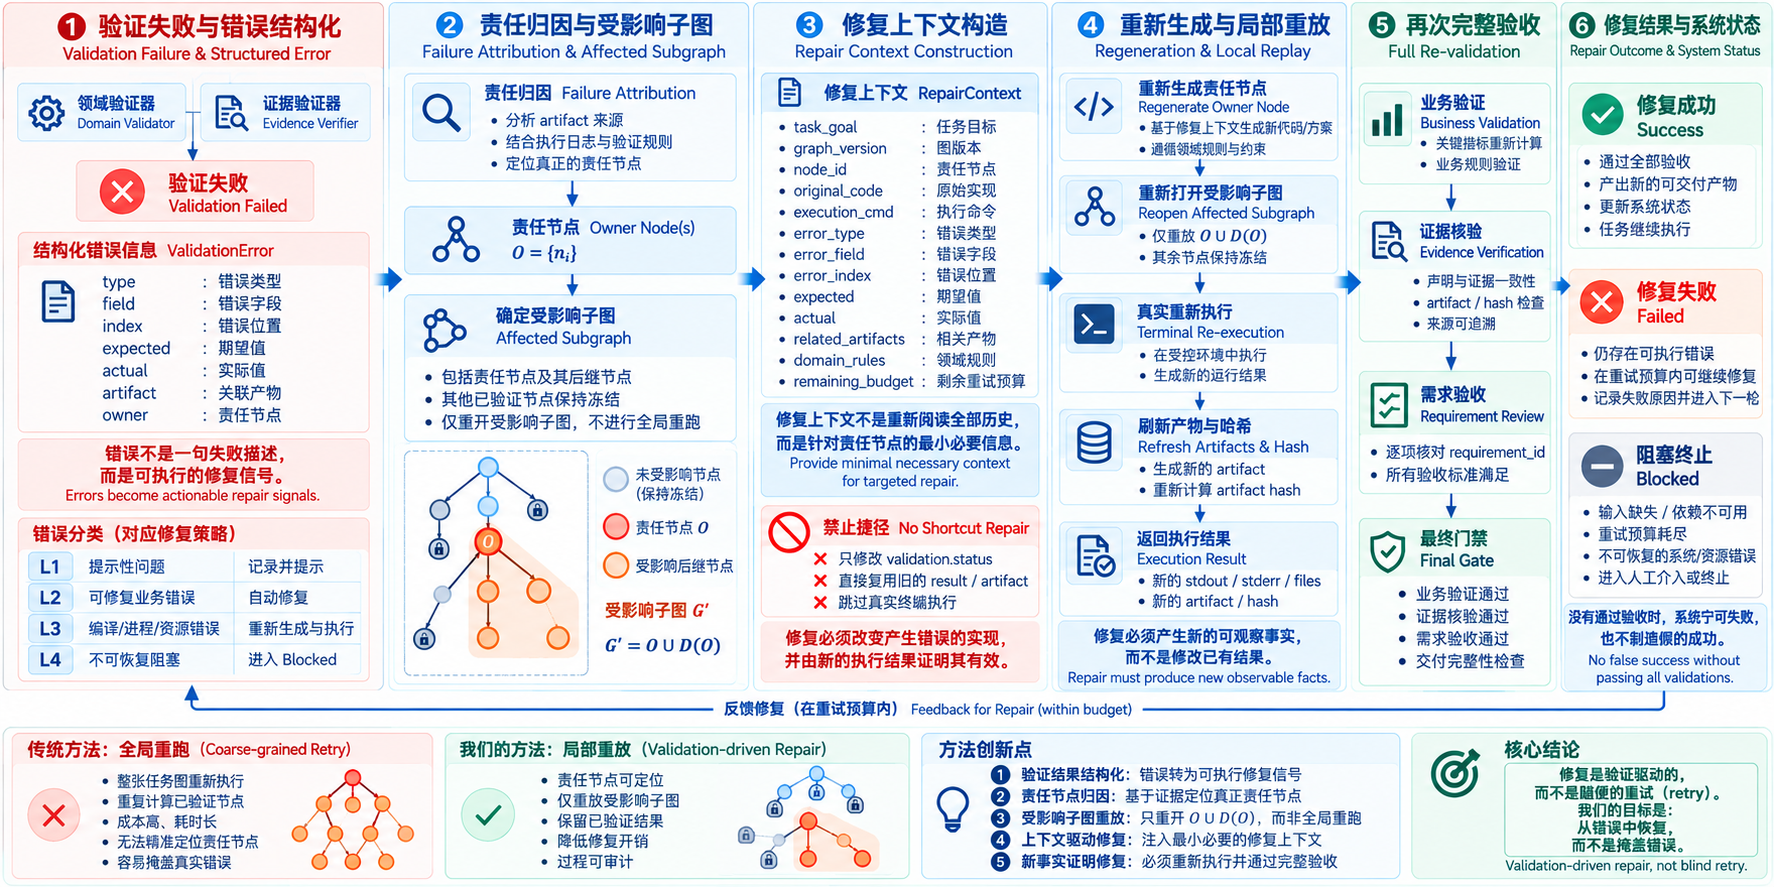
\includegraphics[width=0.98\textwidth]{figures/验证驱动的错误归因、局部重放与自主修复闭环.png}
\caption{验证驱动的错误归因与局部修复：结构化 ValidationError 驱动责任定位、受影响子图重开、候选再生成、真实重执行和完整再验收。}
\label{fig:repair-loop}
\end{figure}

本系统的关键设计是：

\begin{quote}
Validation 不仅用于判断结果是否正确，同时作为控制面下一次状态迁移的结构化控制信号。
\end{quote}

设验证错误对应的责任节点集合为
\[
O\subseteq V,
\]
其后继闭包为
\[
D(O),
\]
则需要重新执行的节点集合为：
\[
V'=O\cup D(O).
\]

对应受影响子图为：
\[
G'=(V',E'),
\]
其中：
\[
E'=
\{(u,v)\in E\mid u,v\in V'\}.
\]

系统只重新打开 $G'$ 中的节点，而：
\[
V\setminus V'
\]
中已经验证并且未受到错误影响的节点继续保持 frozen。

因此，验证错误经过如下链路转化为图结构变化：
\[
\text{Artifact}
\rightarrow
\text{ValidationError}
\rightarrow
\text{Attribution}
\rightarrow
\text{Affected Subgraph}
\rightarrow
\text{Graph Reopen}.
\]

这使验证器不再只是流程末尾的评价组件，而直接参与动态任务图的状态演化。


\subsection{RepairContext}

在责任节点重新执行之前，控制面构造结构化 RepairContext，其中至少包括：

\begin{itemize}
    \item \texttt{task\_goal}；
    \item \texttt{graph\_version}；
    \item \texttt{node\_id}；
    \item 原始候选代码或输出；
    \item 实际执行命令；
    \item 错误类型；
    \item 错误字段与索引；
    \item 期望值或合法范围；
    \item 实际值；
    \item 对应领域规则；
    \item 相关 artifact；
    \item 已冻结节点；
    \item 剩余重试预算；
    \item 明确禁止的捷径操作。
\end{itemize}

RepairContext 使模型无需重新阅读全部历史，而是获得与当前错误直接相关的最小修复信息。


\subsection{Repair 与 Retry 的区别}

本文中的 Repair 与普通 Retry 不同。

普通 Retry 可以表示为：
\[
Execute(v)
\rightarrow
Failed
\rightarrow
Execute(v),
\]
即在原始上下文和实现基本不变的情况下再次执行同一个动作。

Dynamic-HMAS 的 Validation-driven Repair 则为：
\[
\begin{aligned}
&Failure
\rightarrow ErrorStructuring
\rightarrow Attribution
\rightarrow AffectedSubgraph \\[3pt]
&\qquad\rightarrow ContextAugmentation
\rightarrow Regeneration
\rightarrow Execution
\rightarrow Revalidation.
\end{aligned}
\]

也就是说，系统在再次执行之前首先改变模型获得的错误信息和任务上下文，并在必要时生成新的候选实现。因此，Repair 的目标不是“再试一次”，而是根据确定性错误证据改变产生失败结果的实现。


\subsection{防止修复捷径}

为了避免模型通过修改验证状态而绕过真实修复，系统明确禁止：

\begin{itemize}
    \item 仅将 \texttt{validation.status} 修改为 passed；
    \item 继续复用已经失败的旧 \texttt{result.json}；
    \item 删除错误记录以制造通过状态；
    \item 跳过 Terminal Executor；
    \item 只重新生成报告而不重新生成业务 artifact；
    \item 在重试预算耗尽后继续无限尝试。
\end{itemize}

修复必须产生新的真实执行结果，并刷新对应 artifact 和哈希，随后重新经过 Domain Validator、Evidence Verifier、Requirement Reviewer 和 Final Gate。


\subsection{验证驱动修复算法}

\begin{algorithm}[H]
\caption{验证驱动的受影响子图自主修复}
\label{alg:validation-driven-repair}
\KwIn{验证结果 $R_v$，当前任务图 $G_t$，artifact 集合 $A_t$，剩余预算 $B$}
\KwOut{重新验证后的状态或 failed/blocked}

\While{$R_v.failed$ 且 $B>0$}{
    $err \leftarrow classify(R_v.errors)$\;

    $O \leftarrow attribute(err,producer\_node,execution\_log)$\;

    $V' \leftarrow O\cup descendants(O)$\;

    $G' \leftarrow affectedSubgraph(G_t,V')$\;

    $C_{repair} \leftarrow buildRepairContext(err,O,A_t,B)$\;

    冻结所有 $V\setminus V'$ 中已经验证的节点\;

    重新打开 $G'$ 中的受影响节点\;

    根据 $C_{repair}$ 重新生成责任节点候选\;

    真实执行受影响子图\;

    刷新 artifact、producer、版本和哈希\;

    $R_v \leftarrow deterministicValidate()$\;

    $B\leftarrow B-1$\;
}

\eIf{$R_v.failed$}{
    写入 failed 或 blocked 状态\;
}{
    执行证据核验、需求验收和 Final Gate\;
}
\end{algorithm}


\section{局部重放范围与可复用性}

验证驱动修复的一个重要目标是避免单点错误导致整个长程任务重新执行。

定义局部重放比例：
\[
ReplayScope
=
\frac{|V'|}{|V|}.
\]

若采用全局重新执行，则：
\[
ReplayScope_{global}=1.
\]

局部修复情况下，当责任错误只影响少量后继节点时：
\[
ReplayScope_{local}<1.
\]

进一步定义已验证结果复用率：
\[
ReuseRate
=
1-\frac{|V'|}{|V|}.
\]

这两个指标可以用于评价局部修复相对于全局重跑在执行节点数量、Token、时间和重复计算方面的差异。

当前报告仅定义上述指标，不对尚未完成统一控制变量实验的 Global Rerun 与 Local Replay 虚构定量比较结果。后续若在同一输入、模型和重试预算下完成控制实验，可在实验章节中补充具体数值。


\section{最终交付门禁}

Final Gate 是系统中唯一具有全局 \texttt{outcome} 写权限的组件。

沿用全文统一定义，任务最终成功需要满足：
\[
Success
=
BV
\land
EV
\land
RA
\land
DV
\land
NoFailed
\land
NoBlocked,
\]
其中：

\begin{itemize}
    \item $BV$ 表示 Business Validation 通过；
    \item $EV$ 表示 Evidence Verification 通过；
    \item $RA$ 表示 Requirement Acceptance 通过；
    \item $DV$ 表示 Delivery Validation 通过；
    \item $NoFailed$ 表示不存在未处理的 failed 节点；
    \item $NoBlocked$ 表示不存在阻塞最终交付的 blocked 节点。
\end{itemize}

在实现层面，最终交付至少需要满足：

\begin{itemize}
    \item \texttt{business\_validation.status = passed}；
    \item \texttt{evidence\_verification.passed = true}；
    \item \texttt{requirement\_acceptance.status = passed}；
    \item \texttt{review.can\_generate\_final\_report = true}；
    \item \texttt{final\_report.md} 实际存在；
    \item 不存在阻塞交付的 failed 或 blocked 节点；
    \item \texttt{run\_state.outcome = success}。
\end{itemize}

因此，“报告已经生成”并不是成功条件。Reporter 可以产生文档候选，但只有 Final Gate 可以确认整条可信链已经闭合。


\section{真实失败案例：MathorCup 坐标越界修复}

MathorCup 历史运行中曾出现：
\[
\texttt{placements[11].x}
\]
超出车辆允许边界的问题。

如果系统仅接受生成模型的“约束已经满足”描述，该错误可能直接进入最终结果。Dynamic-HMAS 则通过领域验证器从真实 \texttt{result.json} 中检测到坐标异常，并将其结构化为边界错误。

该真实失败案例的控制过程如表~\ref{tab:real-repair-case} 所示。

\begin{table}[htbp]
\centering
\caption{MathorCup 坐标越界错误的验证驱动修复过程}
\label{tab:real-repair-case}
\begin{tabularx}{0.96\textwidth}{p{0.24\textwidth}X}
\toprule
阶段 & 系统行为\\
\midrule

错误对象
&
\texttt{placements[11].x} 超出车辆允许范围\\

发现机制
&
Domain Validator 对实际 placements 执行边界复算\\

错误信息
&
保留字段、索引、允许范围和实际值\\

责任归因
&
依据 result artifact 的 producer 定位到生成 placements 的代码节点\\

受影响范围
&
重新打开代码生成、Terminal Execution、领域验证及对应后继证据节点\\

保留内容
&
与该错误无关且已经验证的节点继续保持 frozen\\

RepairContext
&
注入错误字段、索引、期望范围、实际值、领域边界规则和剩余预算\\

重新执行
&
生成新的候选代码，并通过 Terminal Executor 重新运行\\

重新验收
&
重新生成结果文件、约束日志、成本比较和证据信息，并再次完成业务、证据和需求验收\\

最终状态
&
只有重新验证链路全部通过后，才允许进入最终报告和 Final Gate\\

\bottomrule
\end{tabularx}
\end{table}

该案例体现了 Dynamic-HMAS 的核心区别：错误不会被模型解释文本覆盖，而是被转换为能够改变后续任务图和真实执行结果的控制信号。


\section{可验证指标与对照评价设计}

为了使可信执行与自主修复能够被机器评价，本章定义以下指标。

\begin{itemize}
    \item \textbf{真实执行率}：需要真实执行的节点中，具有 Terminal Execution 记录的比例；
    \item \textbf{业务验证通过率}：进入领域验收的结果中，通过确定性业务验证的比例；
    \item \textbf{证据闭合率}：关键声明中能够闭合到合法 artifact、producer、版本和哈希的比例；
    \item \textbf{自动修复成功率}：进入可恢复错误路径后最终重新通过完整验收的比例；
    \item \textbf{平均修复轮数}：完成一次成功修复所需的平均 Repair 次数；
    \item \textbf{ReplayScope}：一次错误需要重新执行的任务图比例；
    \item \textbf{ReuseRate}：局部修复过程中保留的已验证任务比例；
    \item \textbf{无关节点重复执行率}：不属于受影响子图但被错误重新执行的节点比例；
    \item \textbf{假成功率}：存在业务、证据或需求错误但被写入全局 success 的运行比例；
    \item \textbf{失败阻断准确率}：无法恢复任务是否被正确阻断而不是伪造成功。
\end{itemize}

其中，假成功率的目标为：
\[
FalseSuccessRate=0.
\]

当前千步级运行已经记录恢复后的重复执行为 0；动态异常注入实验中的节点失效、需求变更和数据异常均形成 recovered 轨迹。具体运行证据和实验口径将在后续实验章节统一给出。

对于局部修复效率，一个完整的控制变量实验可以进一步比较：

\begin{table}[htbp]
\centering
\caption{局部修复机制的控制变量评价设计}
\label{tab:repair-ablation-design}
\begin{tabularx}{0.96\textwidth}{p{0.20\textwidth}X X X}
\toprule
方法 & 重放范围 & 已验证结果复用 & 预期评价指标\\
\midrule

Global Rerun
&
重新执行整个任务图
&
低
&
节点数、Token、时间、最终验收\\

Affected-subgraph Repair
&
仅责任节点及其后继
&
高
&
ReplayScope、ReuseRate、Token、时间、最终验收\\

\bottomrule
\end{tabularx}
\end{table}

在没有同条件实测结果之前，本文不将理论上的局部性直接表述为已经测得的 Token 或时间优势。


\section{本章小结}

本章建立了 Dynamic-HMAS 从模型候选走向可信交付的执行与验证机制。其核心并不是在模型之后简单增加一个 Validator，而是定义了完整的事实状态跃迁：
\[
\text{Candidate}
\rightarrow
\text{Observable Fact}
\rightarrow
\text{Verified Fact}
\rightarrow
\text{Deliverable Fact}.
\]

首先，模型生成的代码、文本和结构化结果只能作为 Candidate；Terminal Executor 通过真实进程、实际文件和 artifact 哈希将候选转化为 Observable Fact；Domain Validator 和 Evidence Verifier 分别验证业务正确性和执行来源，使结果成为 Verified Fact；只有 Requirement Contract 和 Final Gate 全部闭合后，该事实才具备最终交付资格。

其次，本章建立了版本化证据闭合机制。最终声明必须能够回溯到具体 producer node、实际 artifact、任务图版本和内容哈希，因此可信性不依赖模型自报，而依赖可复核的执行来源链。

最后，系统将验证结果从“评价信号”进一步提升为“控制信号”。结构化 ValidationError 通过责任归因定位故障节点，并驱动受影响子图重开、RepairContext 构造、候选再生成、真实重执行和完整再验收。该过程不同于简单 Retry，因为再次执行之前已经依据确定性错误改变了任务上下文和候选实现。

因此，本章形成了三项相互关联的核心机制：\textbf{执行锚定的事实状态跃迁、版本化证据闭合以及验证驱动的图级自主修复}。它们共同使 Dynamic-HMAS 不仅能够产生结果，也能够证明结果为何成立；不仅能够处理成功路径，也能够在错误无法修复时拒绝错误交付，从而形成可执行、可验证、可恢复且可拒绝的自治任务闭环。

\chapter{多场景实验、长程压力测试与机制验证}

本章通过跨领域任务运行、千步级长程压力测试、动态异常注入以及机器可审计运行证据，对前文提出的 Dynamic-HMAS 核心机制进行验证。实验目标不仅是证明系统“能够运行”，更重要的是回答动态任务图、ContextCapsule、语义 checkpoint、可信执行和验证驱动修复是否真正形成了可观察、可恢复和可复核的系统行为。

因此，本章不将“程序未发生崩溃”或“模型生成了最终报告”视为任务成功。一次运行只有在 WorkUnit 完整执行、关键任务状态保持、领域业务验证通过、证据来源闭合、需求账本完成验收且最终交付门禁通过时，才被认定为成功。

在已有真实运行数据基础上，本章同时严格区分\textbf{已完成的实测结果}与\textbf{尚待完成的控制变量实验}。对于尚未在相同模型、输入和预算条件下完成实测的 Static DAG、Summary Only 和 Global Rerun 等基线，本文仅给出评价设计，不填入推测数值。


\begin{figure}[htbp]
\centering
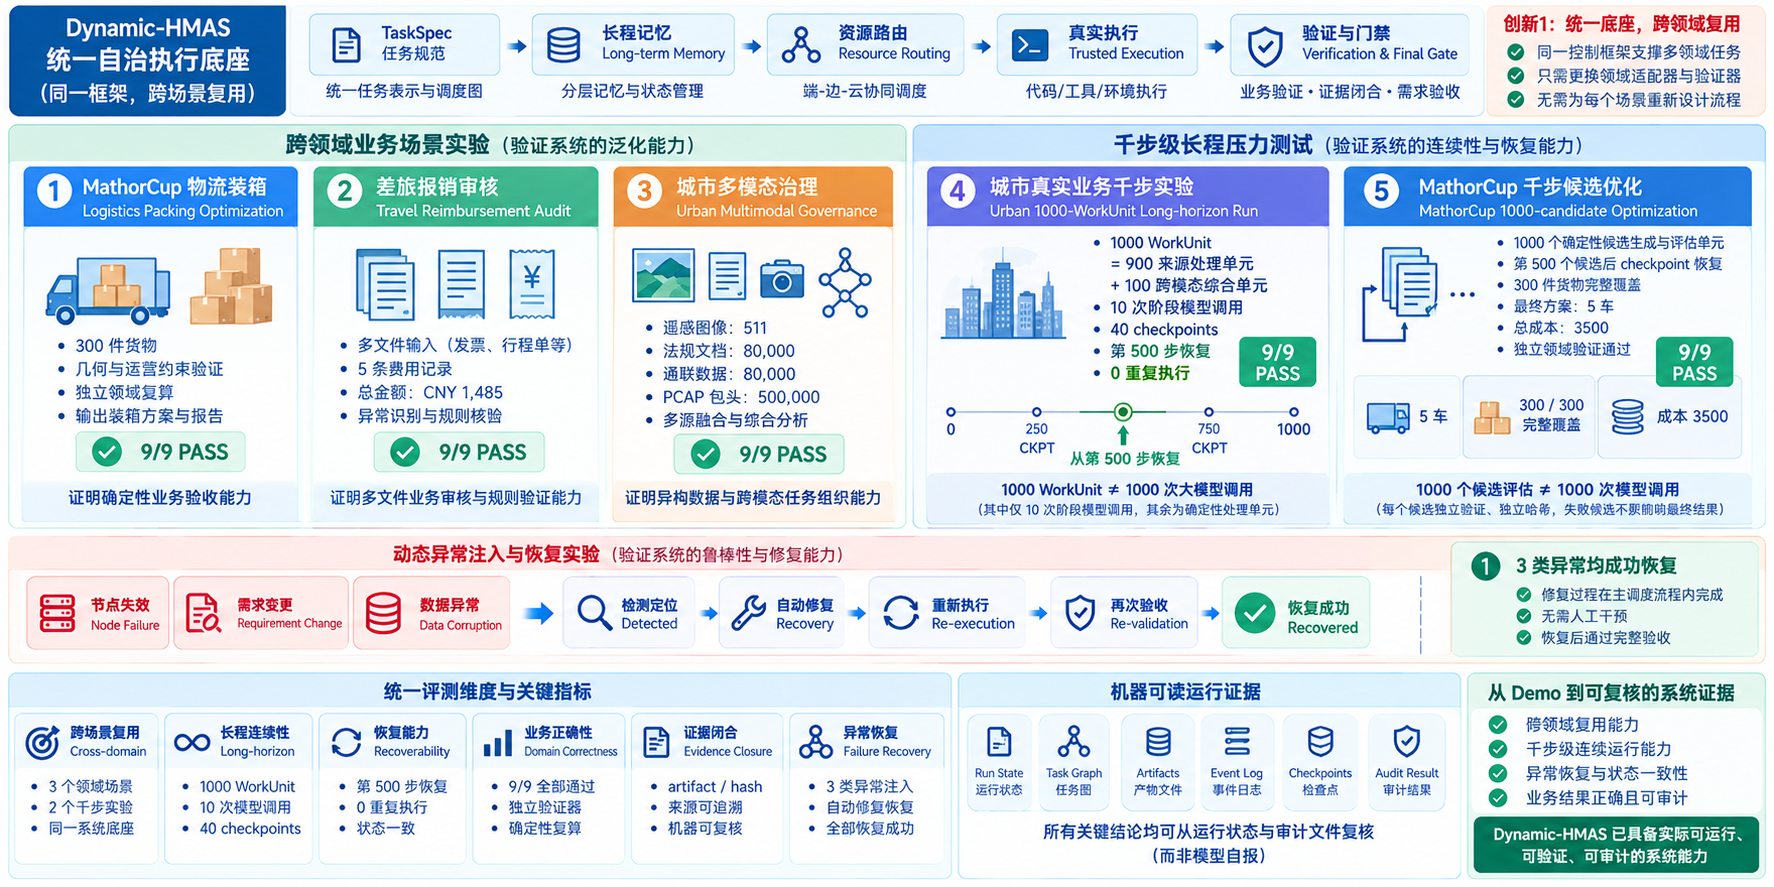
\includegraphics[width=0.98\textwidth]{figures/多场景实验与长程运行证据总览.png}
\caption{Dynamic-HMAS 多场景实验与长程运行证据总览：跨领域任务、千步级 WorkUnit、checkpoint 恢复、异常注入、确定性验收和独立于主执行链的审计脚本共同构成可复核实验链。}
\label{fig:multi-scenario-evidence-overview}
\end{figure}


\section{研究问题与评价维度}

为了使实验与前文提出的核心机制一一对应，本章围绕六个研究问题展开。

\textbf{RQ1：跨领域复用能力。}
在输入格式、业务规则和领域验证函数显著不同的情况下，同一套 TaskSpec、动态任务图、记忆、资源调度、真实执行和最终门禁是否仍能够复用？

\textbf{RQ2：长程状态连续性。}
当任务扩展到千步级 WorkUnit 后，系统是否仍能够保持目标、硬约束、图版本、artifact 来源和验收状态，并在中断后从 checkpoint 无重复恢复？

\textbf{RQ3：动态稀疏通信。}
依赖驱动的动态通信是否能够保持稀疏拓扑，避免所有 Agent 共享完整历史，并在当前任务中完成可信交付？

\textbf{RQ4：ContextCapsule 的状态保持能力。}
受保护状态和预算化上下文机制是否能够保证关键字段不因摘要、压缩和长程执行发生丢失？

\textbf{RQ5：验证驱动修复的局部性。}
当业务执行或验证失败时，系统是否能够根据 ValidationError 定位责任节点，仅重开受影响子图，并保持其他已经验证结果不变？

\textbf{RQ6：动态异常与资源变化鲁棒性。}
面对节点失效、需求变更、数据异常以及执行资源变化，系统是否能够保持任务语义和验收状态，并重新进入可信执行路径？

实验指标相应划分为六类：跨场景正确性、长程连续性、通信效率、状态保持、恢复局部性以及异常鲁棒性。


\subsection{复合成功条件}

沿用前文的可信交付定义，本章将一次任务成功表示为：

\[
Success
=
Complete
\land
Schema
\land
BV
\land
EV
\land
RA
\land
DV,
\]

其中：

\begin{itemize}
    \item $Complete$ 表示要求执行的 WorkUnit 已完整处理；
    \item $Schema$ 表示结构化结果满足输出契约；
    \item $BV$ 表示 Business Validation 通过；
    \item $EV$ 表示 Evidence Verification 通过；
    \item $RA$ 表示 Requirement Acceptance 通过；
    \item $DV$ 表示最终 Delivery Validation 通过。
\end{itemize}

任一条件不满足时，系统均保留对应失败轨迹，而不会将“部分完成”或“报告已生成”计为任务成功。


\section{实验设置与可复现原则}

实验采用“\textbf{统一控制框架、领域插件可替换}”的设计原则。不同实验共享：

\begin{itemize}
    \item TaskSpec 与 Requirement Contract；
    \item 动态 TaskNode 与任务图调度；
    \item ContextCapsule 与 checkpoint；
    \item ResourceRegistry 和资源路由；
    \item artifact 与版本管理；
    \item Terminal Executor；
    \item Evidence Verifier；
    \item Requirement Reviewer；
    \item Final Gate。
\end{itemize}

不同场景主要替换输入适配器、部分节点提示以及 Domain Validator 中的领域规则，从而检验系统核心控制语义能否跨领域保持稳定。

每次实验使用独立的 \texttt{run\_dir}，状态和运行产物均以追加方式保存，并为关键文件计算哈希。运行结束后，由独立于主执行链的 \texttt{run\_audit.py} 对运行目录执行机器检查，避免将手工修改或部分成功结果混入最终实验数据。


\subsection{运行环境与复现方式}

实验运行于 Conda 的 \texttt{agent} 环境，模型服务通过环境变量配置，典型执行命令为：

\begin{lstlisting}
conda activate agent
python main.py --input examples/mathorcup_d
python utils/run_audit.py outputs/runs/RUN_ID
\end{lstlisting}

每次运行至少保存：

\begin{itemize}
    \item \texttt{run\_state.json}；
    \item \texttt{task\_graph.json}；
    \item \texttt{agent\_trace.md}；
    \item \texttt{events.jsonl}；
    \item \texttt{artifacts/}；
    \item \texttt{review/}；
    \item \texttt{checkpoints/}；
    \item \texttt{injections/}。
\end{itemize}

实验材料不在代码、日志和截图中保存 API Key。所有关键结论优先从机器可读运行状态和 artifact 中提取，而不是依赖人工观察 Dashboard。


\section{跨领域总体结果}

首先使用三个业务结构差异较大的场景验证统一控制框架的跨领域适用性。

\begin{longtable}{p{0.20\textwidth}p{0.25\textwidth}p{0.42\textwidth}}
\caption{三个代表性场景的端到端运行结果}
\label{tab:cross-domain-overall-results}\\
\toprule
场景 & 任务性质 & 运行证据与关键结果\\
\midrule
\endfirsthead

\toprule
场景 & 任务性质 & 运行证据与关键结果\\
\midrule
\endhead

MathorCup D
&
物流装箱优化
&
\texttt{outputs/runs/20260908\_124006}；
300 件货物；
领域约束与成本复算；
独立于主执行链的审计脚本 9/9 PASS
\\

差旅报销
&
多文件业务审核
&
\texttt{outputs/runs/20260908\_125323}；
5 条费用；
总金额 CNY 1,485；
完成异常识别；
审计脚本 9/9 PASS
\\

城市多模态
&
异构数据治理
&
\texttt{outputs/runs/20260908\_173502}；
遥感记录 511；
法规 80,000；
匿名通联 80,000；
PCAP 500,000；
审计脚本 9/9 PASS
\\

\bottomrule
\end{longtable}

三个场景的输入结构、业务规则和验证逻辑并不相同。MathorCup 重点验证几何、数量、载重和成本约束；差旅报销重点验证金额、票据和政策条件；城市多模态场景重点处理多源数据的来源、统计和跨模态综合。

实验中保持不变的是任务契约、动态图、记忆、真实执行、证据闭合和最终门禁。因此，跨场景结果主要验证的不是“同一提示词能否解决不同任务”，而是\textbf{同一自治执行状态语义能否支撑不同领域插件}。


\section{长程连续性与千步级压力测试}

为了验证系统在任务规模增长后是否仍能保持状态连续性，本节使用两个千步级实验：城市多模态真实数据长程实验和 MathorCup 候选优化压力实验。


\subsection{城市多模态真实数据千步实验}

城市多模态实验将遥感元数据或 caption、政策法规、匿名通联以及 PCAP 包头统计拆分为 900 个来源处理 WorkUnit，并进一步生成 100 个跨模态综合 WorkUnit，共形成：

\[
N_{unit}=900+100=1000.
\]

系统在每个 WorkUnit 完成后记录输入范围、输出摘要、来源哈希和需求摘要。每 25 个 WorkUnit 保存一次 checkpoint，因此整个运行产生：

\[
N_{checkpoint}=40.
\]

实验在第 500 个 WorkUnit 结束后重新实例化运行进程，并从 checkpoint 20 恢复。恢复时重新加载任务图版本、memory snapshot、artifact manifest、requirement digest 和已完成 WorkUnit 集合，随后重新构造 ready 队列。

已经通过验证的前序 WorkUnit 通过幂等键被跳过，最终记录：

\[
N_{duplicate}=0.
\]

实验包含 10 次阶段模型调用，其余来源处理主要由确定性程序完成。因此，本实验中的 1,000 个 WorkUnit 表示可审计的长程执行单元，而不等价于 1,000 次大模型调用。

\begin{table}[htbp]
\centering
\caption{城市多模态真实数据千步实验结果}
\label{tab:urban-1000-results}
\begin{tabular}{p{0.42\textwidth}p{0.32\textwidth}}
\toprule
指标 & 实测结果\\
\midrule
总 WorkUnit & 1,000\\
来源处理 WorkUnit & 900\\
跨模态综合 WorkUnit & 100\\
阶段模型调用 & 10\\
Checkpoint 数量 & 40\\
恢复 checkpoint & checkpoint 20\\
恢复位置 & 第 500 步\\
恢复后重复执行 & 0\\
\bottomrule
\end{tabular}
\end{table}


\begin{figure}[htbp]
\centering
\resizebox{0.94\textwidth}{!}{%
\begin{tikzpicture}[node distance=9mm and 10mm]
\node[core] (u) {城市多模态\\1000 WorkUnit};
\node[box,below left=of u] (r) {遥感元数据\\511 条};
\node[box,below=of u] (l) {政策法规\\80,000 条};
\node[box,below right=of u] (p) {通联 / PCAP\\80,000 / 500,000};
\node[guard,below=18mm of l] (f) {100 个跨模态综合单元\\10 次阶段模型调用};
\node[core,below=of f] (c) {checkpoint 20 恢复\\第 500 步，重复 0};
\node[guard,right=18mm of c] (m) {40 个 SHA256 checkpoint\\主执行链外审计 9/9 PASS};

\draw[arrow] (u)--(r);
\draw[arrow] (u)--(l);
\draw[arrow] (u)--(p);
\draw[arrow] (r)--(f);
\draw[arrow] (l)--(f);
\draw[arrow] (p)--(f);
\draw[arrow] (f)--(c)--(m);
\end{tikzpicture}
}
\caption{城市多模态真实数据千步实验：多源处理、跨模态综合以及第 500 步 checkpoint 恢复。}
\label{fig:urban-1000}
\end{figure}

该实验主要验证的是\textbf{长程状态管理}而不是千轮语言模型推理：随着执行规模增长，来源范围、图版本、checkpoint、已验证事实和需求摘要仍能够被持续保存，并在进程重新实例化后继续使用。


\subsection{MathorCup 千步候选优化实验}

MathorCup 千步实验生成 1,000 组不同参数的确定性候选方案并逐一评估，而不是机械重复完全相同的任务。

每个候选均经过：

\begin{itemize}
    \item 输出 Schema 检查；
    \item 货物类型与数量覆盖；
    \item 坐标边界检查；
    \item 三维 AABB 重叠检查；
    \item 易碎件规则检查；
    \item 顶部间隙检查；
    \item 车辆载重检查；
    \item 空间和载重利用率计算；
    \item 车辆数量复算；
    \item 总成本复算。
\end{itemize}

系统在第 500 个候选后从 checkpoint 恢复，并保留此前已经验证的候选结果。最终从全部可行候选中选择：

\[
vehicle\_count=5,
\qquad
total\_cost=3500,
\]

且 300 件货物完整覆盖并通过独立领域复算。

\begin{table}[htbp]
\centering
\caption{MathorCup 千步候选优化实验结果}
\label{tab:mathorcup-1000-results}
\begin{tabular}{p{0.42\textwidth}p{0.32\textwidth}}
\toprule
指标 & 实测结果\\
\midrule
候选 WorkUnit & 1,000\\
货物数量 & 300\\
最终车辆数 & 5\\
最终总成本 & 3500\\
中断位置 & 第 500 个候选后\\
恢复方式 & checkpoint 恢复\\
最终结果 & 独立领域验证通过\\
\bottomrule
\end{tabular}
\end{table}

该实验主要评价的是\textbf{长程候选状态管理与确定性验证的规模扩展能力}，不将 1,000 个候选描述为 1,000 次大模型推理。


\subsection{长程连续性指标}

关键字段保持率定义为：

\[
Retention
=
\frac{N_{kept}}{N_{critical}}.
\]

历史运行的末端 ContextCapsule 保留全部 12 个预定义关键字段，因此记录：

\[
Retention=\frac{12}{12}.
\]

恢复重复率定义为：

\[
ReplayRate
=
\frac{N_{duplicate}}{N_{unit}}.
\]

当前两个千步级实验中均未记录已验证 WorkUnit 的重复执行。

\begin{table}[htbp]
\centering
\caption{长程状态连续性的已观测证据}
\label{tab:long-horizon-continuity}
\begin{tabularx}{0.95\textwidth}{p{0.30\textwidth}X}
\toprule
评价项 & 当前证据\\
\midrule
关键字段保持 & 末端 ContextCapsule 保留 12/12 个关键字段\\
任务规模 & 两项 1,000 WorkUnit 实验\\
语义 checkpoint & 城市实验共 40 个 checkpoint\\
中断恢复 & 第 500 步从 checkpoint 20 恢复\\
重复执行 & 已验证 WorkUnit 重复数为 0\\
状态一致性 & 图版本、memory snapshot、artifact manifest 和 requirement digest 联合恢复\\
\bottomrule
\end{tabularx}
\end{table}


\section{动态稀疏通信效率}

本节验证第三章提出的依赖驱动结构化通信是否在实际运行中形成稀疏拓扑。

本文所称“低熵通信”是工程意义上的冗余控制概念，并不直接等价于 Shannon 信息熵。实验主要观察：

\begin{itemize}
    \item 实际活跃通信边数量；
    \item 理论完全连接边数量；
    \item 拓扑密度；
    \item 平均输入上下文；
    \item Token 消耗；
    \item 是否发生全历史广播。
\end{itemize}

当前 MathorCup D 的代表性已审计运行记录了以下实测数据：

\begin{table}[htbp]
\centering
\caption{MathorCup D 动态稀疏通信的代表性结果与基线口径}
\label{tab:low-entropy-communication}
\small
\begin{tabularx}{0.98\textwidth}{
p{0.19\textwidth}
>{\centering\arraybackslash}X
>{\centering\arraybackslash}X
>{\centering\arraybackslash}X
>{\centering\arraybackslash}X
>{\centering\arraybackslash}X}
\toprule
方法
& Token
& 平均输入上下文
& 通信边数
& 运行结果
& 执行时间\\
\midrule

完全连接
（理论上界）
& --
& --
& 182
& --
& --\\

静态 DAG
（待同条件实测）
& --
& --
& --
& --
& --\\

本文动态稀疏策略
（实测）
& 209,937
& 10,929
& 31
& 成功（1/1）
& 720 s\\

\bottomrule
\end{tabularx}
\end{table}

代表性运行中实际观察到 31 条活跃通信边。与 182 条理论完全连接关系相比，实际边数量约为理论上界的：

\[
\frac{31}{182}\approx0.170.
\]

对应关系数量在拓扑规模意义上减少约：

\[
1-\frac{31}{182}\approx83.0\%.
\]

同时，该运行没有发生将完整历史广播给所有 Agent 的行为。

需要特别强调的是，182 条边属于理论完全连接基线，而不是同条件真实运行得到的 Token 或延迟基线。因此，本实验可以支持“实际拓扑保持稀疏”和“未进行全历史广播”的结论，但\textbf{不能仅根据该表宣称相对于 Static DAG 或 Full-connected 策略已经获得确定的 Token 或时间优势}。


\subsection{Static DAG 控制实验设计}

为了进一步验证动态图相对于固定拓扑的有效性，应在以下条件保持一致时执行 Static DAG 与 Dynamic Sparse 对照：

\begin{itemize}
    \item 相同 TaskSpec；
    \item 相同输入文件；
    \item 相同模型与模型参数；
    \item 相同上下文预算；
    \item 相同 retry budget；
    \item 相同最终成功判定条件。
\end{itemize}

建议统一记录：

\begin{table}[htbp]
\centering
\caption{动态稀疏通信控制变量实验设计}
\label{tab:communication-ablation-design}
\begin{tabularx}{0.96\textwidth}{p{0.22\textwidth}X X X}
\toprule
方法 & 通信结构 & 主要评价量 & 当前状态\\
\midrule

Full-connected
& 所有节点两两允许通信
& Token、上下文、时间、成功率
& 尚未完成同条件实测\\

Static DAG
& 任务开始前固定依赖图
& Token、边数、时间、成功率
& 尚未完成同条件实测\\

Dynamic Sparse
& 按任务状态动态激活直接依赖
& Token、边数、上下文、成功率
& 已有代表性实测\\

\bottomrule
\end{tabularx}
\end{table}

在控制实验完成之前，本文保留未测项目，不填入估计结果。


\section{ContextCapsule 长程状态评价}

第四章提出 ContextCapsule 的核心目标并不是保存完整历史，而是同时满足：

\[
P_v\subseteq C_v
\]

以及：

\[
Tokens(C_v)\leq B_v.
\]

即关键 protected state 必须完整保留，而普通上下文受到节点预算约束。

当前真实运行能够直接提供两类证据：

\begin{enumerate}
    \item 末端 ContextCapsule 保留预定义关键字段 12/12；
    \item checkpoint 恢复后已验证 WorkUnit 重复执行数量为 0。
\end{enumerate}

这些结果能够证明 protected state 与语义 checkpoint 在当前运行中实现了状态连续性，但尚不能单独证明其相对于 Full History 或 Summary Only 的定量优势。


\subsection{长程记忆消融设计}

为了验证 ContextCapsule 的必要性，一个严格控制变量实验应比较：

\begin{table}[htbp]
\centering
\caption{ContextCapsule 长程记忆消融实验设计}
\label{tab:memory-ablation}
\begin{tabularx}{0.96\textwidth}{p{0.21\textwidth}X X X}
\toprule
方法 & 状态保持方式 & 主要风险 & 待评价指标\\
\midrule

Full History
& 将全部历史持续注入上下文
& Token 持续增长、噪声累积
& Retention、Token、Success\\

Summary Only
& 使用递归摘要替代历史
& 硬约束可能在摘要中漂移
& Retention、Constraint Drift、Success\\

ContextCapsule
& Protected state + Direct Dependency + Budgeted Retrieval
& 需要额外外部状态管理
& Retention、Token、Constraint Drift、Success\\

\bottomrule
\end{tabularx}
\end{table}

其中建议至少记录：

\[
CriticalRetention,
\quad
AverageInputTokens,
\quad
ConstraintDrift,
\quad
FinalSuccess.
\]

由于当前报告中没有上述三种策略在完全相同输入和模型条件下的完整实测结果，因此本节不对 Full History 和 Summary Only 填入推测性数值。


\section{验证驱动修复与局部重放评价}

第五章将修复定义为：

\[
\begin{aligned}
&ValidationError
\rightarrow Attribution
\rightarrow AffectedSubgraph \\[3pt]
&\qquad\rightarrow RepairContext
\rightarrow ReExecution
\rightarrow ReValidation.
\end{aligned}
\]

该机制的一个核心目标是避免单个局部错误导致整张任务图从头执行。

定义：

\[
ReplayScope
=
\frac{|V'|}{|V|},
\]

其中 $V'$ 为错误责任节点及其后继组成的受影响节点集合。

进一步定义：

\[
ReuseRate
=
1-ReplayScope.
\]

当前系统已经存在真实 Validation-driven Repair 路径和 MathorCup 坐标越界案例，但当前报告尚未给出 Global Rerun 与 Affected-subgraph Repair 在完全相同条件下的统一性能比较。因此，本节将局部修复的实验评价设计明确如下：

\begin{table}[htbp]
\centering
\caption{全局重跑与局部修复的控制变量实验设计}
\label{tab:repair-ablation}
\begin{tabularx}{0.96\textwidth}{p{0.24\textwidth}X X}
\toprule
评价量 & Global Rerun & Affected-subgraph Repair\\
\midrule
重放节点数量 & 待实测 & 待实测\\
ReplayScope & $1$ & 待实测\\
ReuseRate & $0$ & 待实测\\
重复 WorkUnit & 待实测 & 待实测\\
Token 使用 & 待实测 & 待实测\\
Wall Time & 待实测 & 待实测\\
最终业务验证 & 同条件比较 & 同条件比较\\
\bottomrule
\end{tabularx}
\end{table}

该对照用于回答 RQ5：局部修复是否在保持最终正确性的前提下减少不必要的重算。没有完成控制实验前，本文不将理论局部性直接表述为已经测得的 Token 或时间收益。


\section{异构资源路由与故障回退评价}

第五章提出的资源路由采用“硬约束过滤 + 软评分排序”，并将每次资源选择写入运行状态。相应实验需要回答两个问题：

\begin{enumerate}
    \item 路由结果是否满足能力、安全、位置和可用性等硬约束；
    \item 当前资源失效后，系统是否能够在不修改任务语义的情况下选择合法备用资源。
\end{enumerate}

可定义路由合法率：

\[
RoutingLegalRate
=
\frac{N_{legal}}{N_{route}},
\]

以及故障回退成功率：

\[
FallbackSuccessRate
=
\frac{N_{fallback\_success}}{N_{fallback}}.
\]

同时记录：

\begin{itemize}
    \item Security Violation；
    \item Route Traceability；
    \item Model Distribution；
    \item Logical Location Distribution；
    \item Average Latency。
\end{itemize}

当前运行目录已经记录模型名、资源 ID、路由选择和回退事件，可用于审计具体决策；但当前报告所掌握的数据尚不足以给出上述指标在所有运行上的统一汇总统计，因此本节不填入未经重新统计的百分比结果。

\begin{table}[htbp]
\centering
\caption{端边云逻辑资源路由的评价口径}
\label{tab:routing-evaluation}
\begin{tabularx}{0.96\textwidth}{p{0.27\textwidth}X p{0.25\textwidth}}
\toprule
指标 & 含义 & 当前证据状态\\
\midrule

Routing Legal Rate
& 所有路由决策中满足全部硬约束的比例
& 可由运行日志统计，当前未统一汇总\\

Fallback Success Rate
& 资源失败后成功切换并重新通过验收的比例
& 可由故障与回退事件统计\\

Security Violation
& 违反资源安全等级和位置要求的路由次数
& 运行日志可检查\\

Route Traceability
& 是否能够回溯候选、过滤原因、最终资源及模型
& 已保存资源和路由记录\\

Latency
& 节点实际执行耗时
& 已在执行记录中保存\\

\bottomrule
\end{tabularx}
\end{table}

需要说明的是，当前端、边、云均为逻辑资源后端，本实验不将上述结果表述为真实物理边缘集群或参数级分布式推理性能。


\section{动态异常注入与鲁棒性}

为了检验系统是否能够在运行过程中处理非理想事件，实验在主状态机中注入三类异常：

\begin{enumerate}
    \item 节点或执行资源失效；
    \item 用户需求动态变更；
    \item 输入数据异常或损坏。
\end{enumerate}

三类异常均要求经过：

\[
triggered
\rightarrow
detected
\rightarrow
recovery\_started
\rightarrow
recovered.
\]

\begin{table}[htbp]
\centering
\caption{三类动态异常的检测与恢复结果}
\label{tab:dynamic-injection-results}
\begin{tabularx}{0.97\textwidth}{p{0.18\textwidth}X X p{0.16\textwidth}}
\toprule
异常类型 & 检测依据 & 主要恢复动作 & 最终状态\\
\midrule

节点失效
&
执行失败、资源不可用或注入事件
&
记录原资源和错误，重新选择合法资源或重开责任节点
&
recovered\\

需求变更
&
Requirement Contract 或 requirement digest 变化
&
创建新图版本，仅重开受影响节点并重新验收
&
recovered\\

数据异常
&
SHA256 不一致或输入副本损坏
&
隔离异常副本、恢复数据、重新执行受影响路径并校验哈希
&
recovered\\

\bottomrule
\end{tabularx}
\end{table}

三类异常均产生独立 JSON 或 Markdown 轨迹，并与主状态机及 Final Gate 共享相同验收逻辑。只有异常被检测、恢复动作真正发生、对应 artifact 重新生成并通过后续业务和证据验证，事件才被标记为 \texttt{recovered}。

当前结果能够证明系统对三类代表性异常具备可运行恢复路径；由于当前报告主要记录的是三类代表性注入结果，而非大样本随机故障统计，因此更准确的表述是“\textbf{三类代表性异常均完成 recovered}”，而不对其泛化为任意故障条件下的绝对恢复率。


\section{机器可验证指标与审计方法}

本章所有核心结果尽量从机器可读状态计算，而不是依赖人工观察。

例如：

\begin{itemize}
    \item 重复执行由 WorkUnit 幂等键与事件日志交叉检查；
    \item checkpoint 恢复由恢复前后图版本、memory snapshot 和 artifact manifest 检查；
    \item 关键字段保持由 ContextCapsule protected fields 检查；
    \item 异常恢复由 injection state 与最终运行状态联合判断；
    \item 业务正确性由 Domain Validator 复算；
    \item 证据闭合由 claim、producer、artifact、graph version 和 hash 一致性检查；
    \item 最终成功由 Final Gate 和 \texttt{run\_state.outcome} 判断。
\end{itemize}

因此，“运行成功”不是由模型或实验人员主观宣布，而是能够被独立于主执行链的审计程序重新计算。


\section{核心机制与实验依据的对应关系}

为避免前文方法与实验结果相互割裂，表~\ref{tab:mechanism-evidence-mapping} 汇总核心机制及其当前可验证证据。

\begin{longtable}{p{0.25\textwidth}p{0.35\textwidth}p{0.30\textwidth}}
\caption{核心技术机制与实验依据的对应关系}
\label{tab:mechanism-evidence-mapping}\\
\toprule
核心机制 & 当前实验依据 & 当前能够支持的结论\\
\midrule
\endfirsthead

\toprule
核心机制 & 当前实验依据 & 当前能够支持的结论\\
\midrule
\endhead

双平面可信执行
&
MathorCup、差旅报销、城市多模态三个场景；
审计脚本 9/9 PASS
&
同一控制框架能够支撑多领域真实执行和验收
\\

动态稀疏通信
&
代表性运行 31 条活跃边；
理论完全连接关系 182；
无全历史广播
&
实际通信拓扑保持稀疏；
尚不能推出相对 Static DAG 的 Token 优势
\\

Protected ContextCapsule
&
末端关键字段 12/12
&
当前运行中关键状态能够保持；
相对 Summary Only 的优势仍需消融
\\

Semantic Checkpoint
&
40 个 checkpoint；
第 500 步恢复；
重复执行 0
&
能够恢复图、记忆、artifact 与需求状态组成的任务语义
\\

确定性领域验证
&
MathorCup 300 件完整覆盖；
车辆数与成本独立复算
&
最终业务结果不是模型自报
\\

Validation-driven Repair
&
真实坐标越界修复路径；
三类异常均 recovered
&
验证结果能够驱动责任定位与恢复；
局部效率仍需 Global Rerun 对照
\\

异构资源路由
&
运行目录保存模型、资源、路由和回退记录
&
路由过程具备可追溯性；
整体统计指标仍待从日志统一汇总
\\

\bottomrule
\end{longtable}


\section{机制有效性与综合讨论}

现有实验能够支持三个层次的结论。

第一，Dynamic-HMAS 已经形成\textbf{可运行的跨领域自治闭环}。三个业务场景具有不同的数据类型和业务约束，但可以复用统一的任务图、记忆、真实执行、证据闭合和最终门禁。

第二，系统的长程能力来自\textbf{可拆分、可持久化、可验证和可恢复的外部状态}，而不是单纯依赖大模型超长上下文。两个千步级实验以及第 500 步 checkpoint 恢复说明系统能够在执行规模扩大和进程中断后继续保持任务状态。

第三，当前证据已经能够验证部分核心机制的绝对行为，但对于“相对于更简单替代方案是否更优”这一问题，仍需要进一步的严格消融实验。尤其是：

\begin{itemize}
    \item Dynamic Sparse 与 Static DAG 的同条件比较；
    \item ContextCapsule 与 Summary Only 的同条件比较；
    \item Affected-subgraph Repair 与 Global Rerun 的同条件比较；
    \item 多次路由故障注入后的汇总统计。
\end{itemize}

因此，本文将“已经通过真实运行验证的系统能力”与“尚待完成的相对性能结论”严格区分，避免将理论上的机制优势直接表述为未经实验验证的数值收益。


\section{实验边界与结论}

本章所有结论均限定在当前已经完成并可复核的实验范围内。

城市多模态实验使用遥感元数据或 caption、政策法规、匿名通联以及 PCAP 包头统计，不进行个人身份关联、像素级遥感识别或因果推断。

城市长程实验中的 1,000 个 WorkUnit 包含 10 次阶段模型调用，其余步骤主要为确定性来源处理和跨阶段状态管理，因此不能表述为 1,000 次大模型调用。

MathorCup 千步实验中的 1,000 个 WorkUnit 为不同参数候选的确定性生成与评估，主要用于验证候选状态管理、checkpoint 恢复和大规模确定性验收，而不是证明模型进行了 1,000 轮复杂语言推理。

端边云实验当前使用可替换的逻辑资源后端和 TaskNode 级阶段路由，不涉及 Transformer 参数层切分、张量并行或真实物理多机边缘集群。

在上述边界内，实验已经证明 Dynamic-HMAS 能够完成三个跨领域场景的可信运行，并在两个千步级任务中保持可恢复状态；代表性通信运行保持稀疏拓扑，ContextCapsule 保留全部已定义关键字段，checkpoint 能够在第 500 步恢复且不重复已验证工作，节点失效、需求变更和数据异常三类代表性事件均形成 recovered 轨迹。

因此，当前实验最直接支持的结论不是“系统在所有条件下均优于已有方法”，而是：\textbf{Dynamic-HMAS 已经将动态异构协同、受保护长程状态、真实执行、确定性验证、证据闭合和异常恢复统一为一个能够跨场景运行、千步级持续执行并留下机器可审计证据的自治任务系统。}
\chapter{系统级创新、复杂度、部署复现与验收总结}

本章对前述方法、系统实现和实验结果进行收束性分析。前文已经分别给出了双平面总体架构、动态异构群体与深度协同推理、受保护长程状态与 ContextCapsule、可信执行与验证驱动修复，以及多场景和千步级实验。本章不再重复各模块内部算法，而重点回答四个系统级问题：这些机制为何不是若干功能模块的简单并置；系统为获得可信、可恢复和可审计能力付出了怎样的工程代价；评审者如何独立部署、运行和复核系统；任务书中的关键要求分别由哪些机制和运行证据支撑。

本文不依据自身材料对作品进行主观打分，而采用“\textbf{要求—机制—证据—边界}”的方式给出可复核映射。所有结论均限定在当前实现和已有实验范围内，不将逻辑资源路由描述为真实物理集群，不将千步级 WorkUnit 描述为千次大模型推理，也不将潜在应用价值表述为已经产生的经济收益。


\section{系统级创新与统一状态语义}

Dynamic-HMAS 的系统级贡献并不依赖某一个孤立模块。动态任务图、ContextCapsule、资源路由、Terminal Executor、Domain Validator、Evidence Verifier 和 Repair Controller 分别解决不同问题，但真正使其成为一个自治执行系统的是它们共同遵守统一的任务状态、事实状态和权限边界。

系统在时刻 $t$ 的核心运行状态表示为
\[
\sigma_t=(G_t,M_t,A_t,Q_t),
\]
其中 $G_t$ 为当前任务图版本，$M_t$ 为外部记忆与上下文状态，$A_t$ 为带来源、版本和哈希的 artifact 集合，$Q_t$ 为 Requirement Contract 对应的需求验收账本。

模型、调度器、执行器、验证器和恢复控制器均围绕同一个 $\sigma_t$ 工作。因此，系统中的“任务是什么”“当前使用哪个版本”“哪些结果已经真实执行”“哪些事实已经验证”“哪些需求仍未闭合”以及“谁有权宣布最终成功”具有一致定义。

\begin{figure}[htbp]
\centering
\resizebox{0.96\textwidth}{!}{%
\begin{tikzpicture}
\node[core,minimum width=7.6cm,minimum height=1.15cm] (model) at (0,2.2)
{模型驱动智能面\\意图理解 / 规划 / 分析 / 候选生成};

\node[guard,minimum width=7.6cm,minimum height=1.25cm] (state) at (0,0)
{统一运行状态 $\sigma_t=(G_t,M_t,A_t,Q_t)$\\任务图 / 记忆 / artifact / 需求验收账本};

\node[core,minimum width=7.6cm,minimum height=1.15cm] (control) at (0,-2.2)
{确定性控制面\\调度 / 路由 / 真实执行 / 验证 / Final Gate};

\node[box,minimum width=2.8cm] (task) at (7.0,2.0)
{任务闭环\\Task Loop};

\node[box,minimum width=2.8cm] (trust) at (7.0,0)
{可信闭环\\Trust Loop};

\node[box,minimum width=2.8cm] (recovery) at (7.0,-2.0)
{恢复闭环\\Recovery Loop};

\node[guard,minimum width=3.1cm] (deliver) at (11.0,0)
{可信交付\\Audit Evidence};

\draw[arrow] (model)--(state);
\draw[arrow] (state)--(control);
\draw[arrow] (state)--(task);
\draw[arrow] (state)--(trust);
\draw[arrow] (state)--(recovery);
\draw[arrow] (task)--(deliver);
\draw[arrow] (trust)--(deliver);
\draw[arrow] (recovery)--(deliver);

\draw[arrow] (control.west) to[bend right=32] (model.west);
\end{tikzpicture}
}
\caption{Dynamic-HMAS 的系统级统一状态语义：模型驱动智能面和确定性控制面围绕同一运行状态形成任务、可信与恢复三个闭环，并最终产生可验证交付物及审计证据。}
\label{fig:system-level-innovation}
\end{figure}


\subsection{模型能力与系统权限分离}

Dynamic-HMAS 将“模型是否具有某种能力”与“模型是否有权修改系统事实”明确分离。

模型可以理解用户意图、提出任务计划、分析数据、生成代码和提出修复候选，但这些能力并不意味着模型可以直接修改全局成功状态。控制面维护任务图、运行状态、真实执行结果、验证结果和最终门禁。

因此：
\[
\text{Model Intelligence}
\neq
\text{System Authority}.
\]

模型输出首先只是 Candidate；Terminal Executor 产生 Observable Fact；确定性验证将其升级为 Verified Fact；Requirement Contract 和 Final Gate 再决定其是否成为 Deliverable Fact。

这种设计使大模型的开放式能力可以被利用，同时避免系统正确性依赖模型对自身输出的主观判断。


\subsection{事实与证据成为一等系统对象}

普通任务编排主要关注节点、消息和工具调用，而 Dynamic-HMAS 进一步将 artifact、producer、graph version、hash、validation 和 requirement 作为系统运行状态中的显式对象。

对于关键事实 $x$，系统保存其来源关系：
\[
Prov(x)
=
(
producer\_node,
graph\_version,
artifact,
artifact\_hash
).
\]

因此，最终报告中的声明不是脱离执行过程存在的文本，而可以沿以下链路回溯：
\[
Claim
\rightarrow
Requirement
\rightarrow
Producer
\rightarrow
Artifact
\rightarrow
Version
\rightarrow
Hash
\rightarrow
Validation.
\]

系统由此不仅管理“Agent 之间说了什么”，还管理“事实由谁产生、是否真实执行、是否属于当前图版本以及是否经过验证”。


\subsection{验证结果能够反向改变任务结构}

在普通生成式工作流中，验证通常只用于给结果打分或判断通过与否。Dynamic-HMAS 则将 ValidationResult 进一步作为控制面的状态迁移信号。

验证失败后：
\[
\begin{aligned}
&ValidationError
\rightarrow Attribution
\rightarrow AffectedSubgraph \\[3pt]
&\qquad\rightarrow RepairContext
\rightarrow ReExecution
\rightarrow ReValidation.
\end{aligned}
\]

因此，Validator 不仅是运行末端的评价组件，还能够通过责任节点和受影响子图反向影响后续任务拓扑。错误不再简单触发原操作重复执行，而是能够改变后续上下文、节点状态和执行路径。


\subsection{系统级创新的统一表达}

从系统层面看，Dynamic-HMAS 的核心可以概括为：
\[
\boxed{
\begin{aligned}
&\text{Open-ended Intelligence} + \text{Deterministic State} \\[3pt]
&\quad + \text{Execution-grounded Facts} \\[3pt]
&\quad + \text{Validation-driven Adaptation}
\end{aligned}
}
\]
从而形成：
\[
\text{Auditable Autonomous Execution}.
\]

这里的创新重点不是重新发明 DAG、外部记忆、模型调用或验证器本身，而是重新定义这些能力之间的\textbf{状态语义、权限边界、事实来源和反馈关系}，使其能够共同构成长程任务中的可执行、可验证和可恢复闭环。


\section{通用能力基础与本项目系统级重构}

为了准确说明本项目的创新边界，本文将通用技术思想、本项目的重新设计以及最终形成的系统能力区分开来，而不将已有通用概念本身表述为原创。

\begin{longtable}{@{}>{\raggedright\arraybackslash}p{0.18\textwidth}>{\raggedright\arraybackslash}p{0.25\textwidth}>{\raggedright\arraybackslash}p{0.29\textwidth}>{\raggedright\arraybackslash}p{0.20\textwidth}@{}}
\caption{通用能力基础与 Dynamic-HMAS 的系统级重构}
\label{tab:system-reconstruction}\\
\toprule
能力层面 & 通用基础思想 & 本项目重新设计 & 形成的系统能力\\
\midrule
\endfirsthead

\toprule
能力层面 & 通用基础思想 & 本项目重新设计 & 形成的系统能力\\
\midrule
\endhead

模型与工具调用
&
多智能体模型调用和工具执行接口
&
统一封装为带能力、权限、资源和证据要求的 TaskNode
&
模型或执行后端可以替换，但任务状态语义保持不变
\\

任务编排
&
DAG 与工作流调度
&
Requirement Contract、版本化动态图、需求前沿和增量扩展
&
运行过程中可根据结果、需求和异常改变任务结构
\\

智能体通信
&
节点间消息传递
&
MessageEnvelope、直接依赖通信、字段投影和 artifact 引用
&
避免默认全历史广播，形成动态稀疏通信
\\

外部记忆
&
持久化状态和历史检索
&
Protected State、ContextCapsule、来源绑定和只读上下文
&
关键约束不因摘要、压缩和模型切换而静默丢失
\\

检查点恢复
&
程序状态 checkpoint
&
任务图、memory snapshot、artifact manifest、需求摘要联合保存
&
恢复完整任务语义，而不仅是程序执行位置
\\

异构资源选择
&
模型或资源路由
&
硬约束过滤、软评分排序、状态保持式 fallback
&
资源切换不改变任务目标和已验证事实
\\

结果验证
&
Schema 检查或结果评价
&
Candidate--Observable--Verified--Deliverable 事实状态跃迁
&
模型不能通过自报结果绕过真实执行和业务复算
\\

失败恢复
&
Retry 或全局重跑
&
结构化 ValidationError、责任归因与受影响子图重放
&
验证结果能够反向驱动局部图级修复
\\

\bottomrule
\end{longtable}

因此，本项目的系统级贡献主要来自\textbf{统一接口、统一状态、统一责任边界和统一反馈闭环}。各能力不再作为彼此独立的插件存在，而是通过 TaskSpec、TaskNode、ContextCapsule、artifact provenance、ValidationResult 和 Final Gate 形成可追踪的因果关系。


\section{核心模块复杂度分析}

本节分析控制面主要算法的渐近复杂度，不将实际大模型推理时间、网络传输时间和外部工具运行时间混入算法复杂度。

设：

\begin{itemize}
    \item $V$ 为任务图节点数量；
    \item $E$ 为任务图依赖边数量；
    \item $E_{comm}$ 为实际激活通信边数量；
    \item $C$ 为单次资源路由的候选数量；
    \item $R$ 为当前可检索记忆记录数量；
    \item $B$ 为一次操作涉及的 artifact 总字节数；
    \item $P$ 为 MathorCup 中需要进行空间碰撞检测的摆放对象数量；
    \item $S$ 为额外持久化运行状态规模；
    \item $V'$、$E'$ 为一次修复涉及的受影响子图规模。
\end{itemize}

\begin{table}[htbp]
\centering
\caption{核心控制模块的渐近复杂度}
\label{tab:complexity}
\begin{tabularx}{0.96\textwidth}{p{0.31\textwidth}p{0.28\textwidth}X}
\toprule
模块 & 时间复杂度 & 空间复杂度\\
\midrule

单次 DAG 合法性检查
&
$O(V+E)$
&
$O(V+E)$
\\

资源硬约束过滤
&
$O(C)$
&
$O(C)$
\\

合法资源软排序
&
$O(C\log C)$
&
$O(C)$
\\

实际稀疏消息遍历
&
$O(|E_{comm}|)$
&
与结构化消息规模相关
\\

artifact 哈希
&
$O(B)$
&
流式计算时额外空间有界
\\

当前记忆候选扫描
&
最坏 $O(R)$
&
与候选结果数量相关
\\

checkpoint 序列化
&
$O(V+E+S)$
&
$O(V+E+S)$
\\

受影响子图搜索
&
$O(V'+E')$
&
$O(V'+E')$
\\

MathorCup 成对 AABB 检查
&
最坏 $O(P^2)$
&
$O(P)$
\\

\bottomrule
\end{tabularx}
\end{table}

需要指出的是，当前记忆检索的实际时间还会受到 SQLite 查询、检索字段以及底层索引实现影响，因此本文只给出当前保守的最坏候选扫描复杂度 $O(R)$，不对不同数据库或向量索引后端给出未经验证的统一渐近复杂度。

当前 Scheduler 采用较保守的 ready 节点扫描方式。若每轮均扫描全部节点，则完整调度过程最坏可能达到：
\[
O(V^2+E).
\]
现有千步级实验通过幂等键、批量状态写入、已经验证节点冻结以及增量状态更新完成实际运行，但本文不将该实现描述为理论最优调度器。

受影响子图的 $O(V'+E')$ 仅描述图遍历和状态重开成本，不包含重新调用模型、工具或领域验证器产生的实际执行时间。


\section{可信自治执行的工程代价}

Dynamic-HMAS 相比只进行模型生成的普通 Agent Demo，需要额外维护任务图、事件日志、外部记忆、artifact 来源、checkpoint、验证结果和证据文件。因此，可信性和可恢复性并非没有代价。

\begin{longtable}{p{0.24\textwidth}p{0.31\textwidth}p{0.37\textwidth}}
\caption{可信执行机制带来的工程代价与对应收益}
\label{tab:engineering-cost}\\
\toprule
机制 & 新增工程代价 & 获得的系统能力\\
\midrule
\endfirsthead

\toprule
机制 & 新增工程代价 & 获得的系统能力\\
\midrule
\endhead

版本化任务图
&
图状态、版本和依赖关系持久化
&
需求变化可追踪，旧结果不会静默覆盖新任务
\\

Protected State / ContextCapsule
&
状态检索、字段筛选和上下文组装
&
关键目标和硬约束不依赖模型长窗口保持
\\

artifact 哈希
&
额外哈希计算和文件清单维护
&
能够检测文件变化并建立证据完整性
\\

Semantic Checkpoint
&
周期性序列化及额外存储空间
&
进程中断后能够恢复图、记忆、artifact 与需求状态
\\

Domain Validator
&
增加确定性领域复算
&
防止格式正确但业务错误的结果被当作成功
\\

Evidence Closure
&
维护 producer、version、path 和 hash 关系
&
最终声明能够回溯到实际执行证据
\\

Validation-driven Repair
&
错误分析、图遍历及局部重新执行
&
避免所有错误均退化为全局从头重跑
\\

\bottomrule
\end{longtable}

这些额外开销本质上是从“只追求生成速度”向“追求可验证任务交付”转移的工程成本。其目标不是使每一步都具有最低延迟，而是在超长程复杂任务中换取结果可复算、错误可定位、任务可恢复和交付可审计。

城市多模态真实数据千步实验包含 1,000 个 WorkUnit、10 次阶段模型调用和 40 个 checkpoint；MathorCup 千步实验包含 1,000 个确定性候选生成与评估单元。系统通过结构化摘要、字段投影、artifact 引用和哈希避免将大对象和完整历史反复注入模型上下文。


\section{部署架构与最小复现流程}

Dynamic-HMAS 当前可以在 Conda 环境中运行，并通过 OpenAI-compatible 接口连接模型服务。系统部署不要求依赖 Dashboard 判断结果正确性；Dashboard 只是观察界面，机器可读运行状态才是最终事实来源。

最小复现过程可以表示为：
\[
\text{Environment}
\rightarrow
\text{Model Configuration}
\rightarrow
\text{Input}
\rightarrow
\text{Run}
\rightarrow
\text{Audit}
\rightarrow
\text{Inspect Artifacts}.
\]

典型运行方式如下：

\begin{lstlisting}[caption={Dynamic-HMAS 最小运行与审计流程}]
conda activate agent
python -m pip install -r requirements.txt

python main.py --input examples/mathorcup_d

python utils/run_audit.py outputs/runs/<run_id>
\end{lstlisting}

模型端点和密钥通过环境变量或运行配置注入，不应写入源码、运行轨迹或最终提交包。

一次完整运行至少生成：

\begin{lstlisting}[caption={典型机器可审计运行目录}]
outputs/runs/<run_id>/
    run_state.json
    task_graph.json
    agent_trace.md
    events.jsonl
    artifacts/
    review/
    checkpoints/
    injections/
\end{lstlisting}

其中：

\begin{itemize}
    \item \texttt{run\_state.json} 保存全局状态、节点状态、路由、重试和最终 outcome；
    \item \texttt{task\_graph.json} 保存任务节点、依赖关系和版本；
    \item \texttt{agent\_trace.md} 保存中间决策摘要；
    \item \texttt{events.jsonl} 保存状态迁移和异常事件；
    \item \texttt{artifacts/} 保存真实执行结果；
    \item \texttt{review/} 保存业务、证据和需求验收结果；
    \item \texttt{checkpoints/} 保存长程语义快照；
    \item \texttt{injections/} 保存异常注入及恢复轨迹。
\end{itemize}

评审者可以在不依赖模型解释和前端截图的情况下，通过运行目录重新检查“任务是否实际执行、结果是否经过验证、异常是否真正恢复以及最终状态为何被判定为 success”。


\section{复现、审计与提交机制}

Dynamic-HMAS 将“可复现”定义为不仅能够重新启动程序，还能够回答以下问题：

\begin{enumerate}
    \item 当前结果由哪个节点产生；
    \item 该节点是否真实执行；
    \item artifact 是否属于当前图版本；
    \item artifact 是否经过确定性验证；
    \item 关键声明是否具有一致的 producer、path 和 hash；
    \item 运行过程中是否出现异常及恢复；
    \item 最终 success 是否经过 Final Gate。
\end{enumerate}

\texttt{run\_audit.py} 独立于主执行链读取已经生成的运行目录，并检查关键交付条件。其作用是重新计算已有证据，而不是直接参与主任务执行。因此，更准确的表述是“\textbf{独立于主执行链的机器审计}”，而不是第三方机构审计。

\texttt{package\_submission.py} 只应接受达到提交条件的运行目录，并在打包过程中扫描明显的密钥模式。失败运行可以作为 Repair 和异常恢复的研究证据保存，但不能被重新包装为成功运行。

因此，提交材料可以形成三个层次：

\begin{enumerate}
    \item \textbf{论文与技术说明}：解释架构、算法、复杂度、实验与能力边界；
    \item \textbf{可运行代码与部署说明}：允许评审者重新执行代表性任务；
    \item \textbf{真实运行证据}：提供已经完成的 run directory、checkpoint、artifact、validation 和 audit 结果。
\end{enumerate}


\section{轻量 Dashboard 与运行可观测性}

当前系统的前端采用轻量 Dashboard 设计，其主要目标不是提供复杂的商业化交互界面，而是将后端控制状态以评审者容易理解的方式进行可视化。

当前可观测内容主要包括：

\begin{itemize}
    \item 当前运行状态与最终 outcome；
    \item TaskNode 或任务图执行状态；
    \item 模型和逻辑资源路由结果；
    \item Agent 或节点执行轨迹；
    \item artifact 及运行产物；
    \item checkpoint 和异常恢复状态；
    \item Business Validation、Evidence Verification 和 Final Gate 结果。
\end{itemize}

需要强调的是：
\[
\text{Dashboard}
\neq
\text{Source of Truth}.
\]

Dashboard 只负责观察和展示，不能通过前端显示内容绕过底层状态机修改任务是否成功。系统的事实来源仍然是 \texttt{run\_state.json}、实际 artifact、验证结果、事件日志和 Final Gate。

因此，即使当前前端保持轻量设计，系统仍然具有独立于可视化界面的完整机器可审计性。现场演示可以使用 Dashboard 展示短时实时执行过程，而千步级长程能力则由 checkpoint、事件日志、运行目录和机器审计结果共同证明。


\section{兼容性与可扩展接口}

为了避免系统能力绑定于单一模型、单一业务或单一资源环境，Dynamic-HMAS 在模型、领域和资源层均保留结构化扩展边界。

\begin{longtable}{@{}>{\raggedright\arraybackslash}p{0.21\textwidth}>{\raggedright\arraybackslash}p{0.27\textwidth}>{\raggedright\arraybackslash}p{0.27\textwidth}>{\raggedright\arraybackslash}p{0.17\textwidth}@{}}
\caption{Dynamic-HMAS 的主要扩展接口}
\label{tab:extension-interface}\\
\toprule
扩展对象 & 需要提供的接口或配置 & 原有核心无需修改的部分 & 当前证据\\
\midrule
\endfirsthead

\toprule
扩展对象 & 需要提供的接口或配置 & 原有核心无需修改的部分 & 当前证据\\
\midrule
\endhead

模型后端
&
OpenAI-compatible endpoint、model name 与资源描述
&
TaskSpec、TaskNode、Scheduler 和 Final Gate
&
当前已使用不同 Qwen 配置进行逻辑资源路由
\\

新业务领域
&
输入 adapter、节点能力配置和 Domain Validator
&
任务图、Memory、Executor、Evidence 和恢复机制
&
MathorCup、差旅报销、城市多模态三个场景
\\

新逻辑资源
&
ResourceDescriptor，包括能力、安全、时延和可用性
&
TaskSpec 和领域业务逻辑
&
device / edge / cloud 逻辑资源描述
\\

新验证规则
&
确定性规则和标准化 ValidationResult
&
Scheduler、Repair Controller 和 Final Gate
&
几何、金额、政策和证据验证
\\

新证据类型
&
artifact 来源描述与 EvidenceVerifier 规则
&
任务状态和最终交付门禁
&
文件、哈希、producer 和 graph version 证据
\\

\bottomrule
\end{longtable}

当前兼容性结论仅限于已经接入和验证的接口范围。本文不宣称未经实际配置和运行的任意模型、任意边缘硬件或任意业务插件天然兼容。


\section{应用模式与潜在业务价值}

Dynamic-HMAS 的应用价值主要来自将“模型生成建议”进一步推进到“自动执行、确定性检查、证据保留和异常恢复”。当前三个代表性场景体现了不同类型的自动化价值。

\begin{longtable}{@{}>{\raggedright\arraybackslash}p{0.17\textwidth}>{\raggedright\arraybackslash}p{0.24\textwidth}>{\raggedright\arraybackslash}p{0.29\textwidth}>{\raggedright\arraybackslash}p{0.22\textwidth}@{}}
\caption{代表性场景的业务痛点、自动化能力与当前证据}
\label{tab:application-value}\\
\toprule
场景 & 典型人工痛点 & Dynamic-HMAS 自动化能力 & 当前已有证据\\
\midrule
\endfirsthead

\toprule
场景 & 典型人工痛点 & Dynamic-HMAS 自动化能力 & 当前已有证据\\
\midrule
\endhead

MathorCup 装箱
&
多约束方案生成后需要逐项检查几何、数量、重量和成本
&
自动生成候选、真实执行、几何约束复算、成本复算和失败修复
&
300 件完整覆盖，5 车，总成本 3500，并通过领域验证
\\

差旅报销
&
多文件金额汇总、政策核验和异常判断需要人工交叉检查
&
票据解析、金额统计、规则核验、异常识别和证据输出
&
5 条费用，总金额 CNY 1,485，并形成异常识别结果
\\

城市多模态
&
多来源数据处理链长，来源、版本和中断恢复难以人工持续维护
&
多源 WorkUnit 管理、来源哈希、跨模态综合、checkpoint 和恢复
&
1,000 WorkUnit、40 checkpoint、第 500 步恢复、重复执行 0
\\

\bottomrule
\end{longtable}

上述结果表明系统具备降低重复核验工作、保持长链路状态和自动形成证据材料的潜力，但本文没有测量真实生产环境中的人工时长、运营成本或经济收益，因此不对“节省多少人力”“提高多少经济效益”等尚未实测的指标作量化承诺。


\section{任务书要求、实现机制与验收证据}

表~\ref{tab:requirement-evidence-map} 将任务书中的关键能力要求映射到系统实现、已有证据和当前边界。该表用于帮助评审者快速定位证据，而不是替代最终评分。

\begin{longtable}{@{}>{\raggedright\arraybackslash}p{0.19\textwidth}>{\raggedright\arraybackslash}p{0.28\textwidth}>{\raggedright\arraybackslash}p{0.29\textwidth}>{\raggedright\arraybackslash}p{0.16\textwidth}@{}}
\caption{任务书关键要求、系统机制、验收证据与能力边界}
\label{tab:requirement-evidence-map}\\
\toprule
任务书要求 & 系统实现机制 & 当前可观测证据 & 当前边界\\
\midrule
\endfirsthead

\toprule
任务书要求 & 系统实现机制 & 当前可观测证据 & 当前边界\\
\midrule
\endhead

超长程上下文连续
&
Protected State、ContextCapsule、语义 checkpoint、幂等恢复
&
关键字段 12/12；40 checkpoint；第 500 步恢复；重复执行 0
&
已验证至千步级，不宣称无限长度
\\

动态异构群体
&
角色契约、TaskNode、版本化动态任务图和运行时能力选择
&
多角色任务图、跨场景节点配置、图版本和恢复记录
&
群体规模由实际 TaskNode 决定
\\

深度协同推理
&
Model Proposal $\rightarrow$ Execution $\rightarrow$ Validation $\rightarrow$ Graph Update
&
任务图扩展、真实执行、validation trace 和 repair trace
&
不将自由多轮聊天等同于深度推理
\\

低熵通信
&
直接依赖通信、MessageEnvelope、字段投影和 artifact 引用
&
代表性运行 31 条活跃边；理论完全连接 182；全历史广播 0
&
尚缺 Static DAG 同条件完整实测
\\

端边云协同
&
ResourceRegistry、硬约束过滤、软评分、状态保持式 fallback
&
模型名、resource ID、候选过滤和回退记录
&
当前为逻辑资源后端，非物理集群
\\

无人工干预闭环
&
TaskSpec、Scheduler、Terminal Executor、Validator、Evidence 和 Final Gate
&
三个代表性场景均形成完整运行目录和 9/9 审计结果
&
领域正确性依赖已实现的 Domain Validator
\\

动态异常处理
&
ValidationError、责任归因、受影响子图、checkpoint 和恢复状态机
&
节点失效、需求变更和数据异常三类代表性事件均 recovered
&
不宣称覆盖所有未知故障类型
\\

可信交付
&
Candidate--Observable--Verified--Deliverable 状态跃迁
&
真实 artifact、业务复算、Evidence Verification、Requirement Acceptance
&
仅已接入领域具有对应确定性验证器
\\

多场景运行
&
统一控制面 + 可替换输入 adapter 和 Domain Validator
&
MathorCup、差旅报销、城市多模态及两项千步实验
&
不同场景的数据解析范围存在明确边界
\\

可部署与复现
&
Conda、OpenAI-compatible 接口、运行目录和机器审计脚本
&
运行命令、run directory、run\_audit.py
&
需要可用模型服务及对应环境配置
\\

材料文档
&
总体架构、核心算法、伪代码、复杂度、实验与边界说明
&
LaTeX 源码、PDF、运行代码和实验目录
&
现场演示可进一步展示运行过程
\\

\bottomrule
\end{longtable}


\section{与评分维度的证据关系}

表~\ref{tab:requirement-evidence-map} 已经给出任务书要求与具体运行证据之间的映射。本节仅从评分维度进行简要归纳，不再重复前文技术内容。

\textbf{作品完整性}主要由高层意图到 TaskSpec、动态任务图、真实执行、反馈恢复和最终交付的完整闭环，以及三个跨领域任务和两项千步级运行支撑。

\textbf{应用创新性}主要由物流优化、财务审核和城市多模态治理三个不同业务形态的统一接入，以及轻量 Dashboard、自动验收和机器审计机制支撑。潜在社会和经济价值仍需要真实生产部署进一步测量。

\textbf{技术创新性}主要体现在统一状态语义、模型能力与系统权限分离、动态异构任务图、Protected ContextCapsule、执行锚定事实链、版本化证据闭合以及 Validation-driven Repair。

\textbf{系统性能与效率}主要由千步级运行连续性、第 500 步恢复、已验证 WorkUnit 重复执行为 0、代表性稀疏通信结果、资源路由记录和三类异常恢复证据支撑。

上述内容仅用于说明“什么证据对应什么能力”，不构成对最终比赛得分的承诺。


\section{当前能力边界}

为了避免将实验结论扩展到尚未实现的能力，本文对当前系统边界作统一说明。

\begin{enumerate}
    \item 当前长程实验已经验证到 1,000 WorkUnit 规模，因此本文统一表述为“千步级”，不将其夸大为已经完成任意规模或无限长度任务。

    \item 城市多模态千步实验中的 1,000 个 WorkUnit 包含 10 次阶段模型调用，其余主要为确定性来源处理和跨阶段状态管理，不等价于 1,000 次大模型推理。

    \item MathorCup 千步实验中的 1,000 个 WorkUnit 为确定性候选生成与评估，用于验证状态管理、checkpoint 和大规模业务验收，不等价于 1,000 轮语言模型推理。

    \item 当前端、边、云表示可替换的逻辑资源后端和 TaskNode 级阶段路由，不涉及 Transformer 参数层切分、张量并行或已经部署的真实物理多机边缘集群。

    \item 城市实验中的遥感部分使用元数据或 caption，PCAP 部分使用包头统计，不将其描述为像素级遥感识别、个人身份关联或因果推断。

    \item 当前 Dashboard 为轻量运行观察界面，其展示结果不能替代底层机器状态和 Final Gate。

    \item Dynamic-HMAS 已经证明三个代表性领域可以共享核心控制框架，但不据此宣称任意新领域均可零成本接入；新的业务领域仍需要实现相应输入 adapter 和确定性 Domain Validator。

    \item 当前实验能够证明系统机制在已有场景中真实运行，但对于 Dynamic Sparse 相对 Static DAG、ContextCapsule 相对 Summary Only、Affected-subgraph Repair 相对 Global Rerun 的定量优势，仍需统一条件下的进一步控制实验。
\end{enumerate}

这些限制并不否定当前实验结果，而是用于明确已有证据能够支持的结论范围。


\section{本章总结}

本章从系统级视角对 Dynamic-HMAS 的创新、复杂度、部署复现、应用模式和任务书验收证据进行了统一收束。

系统级贡献并不在于简单汇集多智能体、任务图、外部记忆、模型路由、验证器和 checkpoint 等通用能力，而在于通过统一状态
\[
\sigma_t=(G_t,M_t,A_t,Q_t)
\]
重新定义模型、任务、事实、证据和恢复之间的关系。

模型负责开放式语义理解和候选生成，但不拥有系统事实和最终成功状态的直接写权限；控制面通过版本化任务图维护任务结构，通过 ContextCapsule 和语义 checkpoint 保持长程状态，通过 Terminal Executor 将候选锚定到真实执行，通过 Domain Validator 与 Evidence Verifier 建立业务正确性和事实来源链，并通过 ValidationError、责任归因和受影响子图使错误能够反向改变后续任务结构。

因此，Dynamic-HMAS 最终形成的不是一个仅能“生成答案”的 Agent 集合，而是一套：
\[
\boxed{
\text{可规划}
+
\text{可执行}
+
\text{可验证}
+
\text{可恢复}
+
\text{可拒绝}
+
\text{可审计}
}
\]
的长程自治任务执行框架。

在当前可复现实验范围内，系统已经在 MathorCup 装箱、差旅报销和城市多模态三个场景中形成完整可信执行链，并通过两个千步级任务、checkpoint 恢复、动态异常注入和机器审计留下可复核证据。与此同时，本文对物理端边云部署、千次大模型调用、无限长记忆和未经实测的相对性能优势保持明确边界，从而使系统创新与实验结论建立在可复现事实而非宣传性描述之上。
\end{document}
